\documentclass[a4paper, 9pt]{scrartcl}\usepackage[]{graphicx}\usepackage[]{xcolor}
% maxwidth is the original width if it is less than linewidth
% otherwise use linewidth (to make sure the graphics do not exceed the margin)
\makeatletter
\def\maxwidth{ %
  \ifdim\Gin@nat@width>\linewidth
    \linewidth
  \else
    \Gin@nat@width
  \fi
}
\makeatother

\definecolor{fgcolor}{rgb}{0.345, 0.345, 0.345}
\newcommand{\hlnum}[1]{\textcolor[rgb]{0.686,0.059,0.569}{#1}}%
\newcommand{\hlstr}[1]{\textcolor[rgb]{0.192,0.494,0.8}{#1}}%
\newcommand{\hlcom}[1]{\textcolor[rgb]{0.678,0.584,0.686}{\textit{#1}}}%
\newcommand{\hlopt}[1]{\textcolor[rgb]{0,0,0}{#1}}%
\newcommand{\hlstd}[1]{\textcolor[rgb]{0.345,0.345,0.345}{#1}}%
\newcommand{\hlkwa}[1]{\textcolor[rgb]{0.161,0.373,0.58}{\textbf{#1}}}%
\newcommand{\hlkwb}[1]{\textcolor[rgb]{0.69,0.353,0.396}{#1}}%
\newcommand{\hlkwc}[1]{\textcolor[rgb]{0.333,0.667,0.333}{#1}}%
\newcommand{\hlkwd}[1]{\textcolor[rgb]{0.737,0.353,0.396}{\textbf{#1}}}%
\let\hlipl\hlkwb

\usepackage{framed}
\makeatletter
\newenvironment{kframe}{%
 \def\at@end@of@kframe{}%
 \ifinner\ifhmode%
  \def\at@end@of@kframe{\end{minipage}}%
  \begin{minipage}{\columnwidth}%
 \fi\fi%
 \def\FrameCommand##1{\hskip\@totalleftmargin \hskip-\fboxsep
 \colorbox{shadecolor}{##1}\hskip-\fboxsep
     % There is no \\@totalrightmargin, so:
     \hskip-\linewidth \hskip-\@totalleftmargin \hskip\columnwidth}%
 \MakeFramed {\advance\hsize-\width
   \@totalleftmargin\z@ \linewidth\hsize
   \@setminipage}}%
 {\par\unskip\endMakeFramed%
 \at@end@of@kframe}
\makeatother

\definecolor{shadecolor}{rgb}{.97, .97, .97}
\definecolor{messagecolor}{rgb}{0, 0, 0}
\definecolor{warningcolor}{rgb}{1, 0, 1}
\definecolor{errorcolor}{rgb}{1, 0, 0}
\newenvironment{knitrout}{}{} % an empty environment to be redefined in TeX

\usepackage{alltt}
\usepackage[ngerman]{babel}

% -----------------------------------------------------------------------

% -----------------------------------------------------------------------
%% ------------------------------------------------------------
%% by J.Kruppa on Friday, February 11, 2022 (11:31)
%% \def\mainDir{\Sexpr{exam_path}}
\def\source{/Users/jokruppa/source/tex}
\usepackage[margin=2cm, includefoot]{geometry}
\setlength{\parindent}{0cm}
\usepackage{booktabs}
\usepackage{amsmath}
\usepackage{scalerel,amssymb}
\usepackage{setspace}
\def\csquare{{\Large $\boxtimes$}}
\def\msquare{{\Large $\square$}}
\usepackage[normalem]{ulem}
\usepackage{array}
\usepackage{xcolor}
\usepackage{float}
\usepackage{currfile}
\usepackage{tikz}
\usepackage[nomessages]{fp}

%% beamer defs
\def\lecture{Klausurfragen der Bio Data Science}

%% exam defs
\def\examtitle{\lecture}
\def\exammodule{
\vspace{-1.75cm}  
\begin{graybox}{}
\vspace{2Ex}
\textbf{\large Name:} \rule[0ex]{16.75em}{.4pt}
\hfill \textnormal{\textit{Nicht bestanden:}} \msquare \\[2.5Ex]
\textbf{\large Vorname:} \rule[0ex]{15em}{.4pt} \\[2.5Ex]
\textbf{\large Matrikelnummer:} \rule[0ex]{10.8em}{.4pt}
\hfill Endnote: \rule[0ex]{7em}{.4pt} 
\end{graybox}
\vspace{3Ex}
\phantom{text}
}
\def\examsemester{Sommersemester \& Wintersemester}
\def\examdate{\today}
%% ------------------------------------------------------------
\definecolor{darkblue}{rgb}{0,0,.5}
\definecolor{darkpurple}{rgb}{0.4117, 0.2, 0.4117}
\definecolor{uni}{rgb}{0,0.3137,0.6078}
\definecolor{gray}{gray}{0.7}

\usepackage{tcolorbox}
\definecolor{logo1}{RGB}{0, 158, 227}
\definecolor{gray5}{RGB}{247, 247, 247}
\definecolor{gray2}{RGB}{102, 102, 102}

\newtcolorbox{graybox}[1]{
  colback=gray5,%%red!5!white,
  colframe=gray2,%%red!75!black,
  fonttitle=\bfseries\Large,
  %%valign=center,
  fontupper=\large,
  before skip=10pt plus 2pt,
  after skip=20pt plus 4pt,
  title=#1}

\newtcolorbox{takehomebox}[1]{
  colback=gray5,%%red!5!white,
  colframe=logo1,%%red!75!black,
  fonttitle=\bfseries\Large,
  %%valign=center,
  fontupper=\large,
  before skip=10pt plus 2pt,
  after skip=10pt plus 2pt,
  title=#1}

\def\Rlogo{
\includegraphics[width = 0.5cm]{\string~/Documents/GitHub/exam/img/Rlogo}\;}

\usepackage[scaled=.90]{helvet} 
\usepackage{fancyhdr}
\usepackage{lastpage}
\usepackage{hyperref}
\hypersetup{
    colorlinks=true,       % false: boxed links; true: colored links
    linkcolor=black,          % color of internal links 
    urlcolor=magenta           % color of external links
}
\renewcommand{\familydefault}{\sfdefault}

\title{
\large \exammodule \\[5Ex]
\Huge \examtitle \\[2Ex] 
\Large Hochschule Osnabr{\"u}ck
}
\author{Pr{\"u}fer: Prof. Dr. Jochen Kruppa \\
Fakult{\"a}t f{\"u}r Agrarwissenschaften und Landschaftsarchitektur \\ 
j.kruppa@hs-osnabrueck.de}
\date{Version vom \examdate}

%% ------------------------------------------------------------
%% by J.Kruppa on Tuesday, September 23, 2014 (12:50)
%% Header
\renewcommand{\headrulewidth}{0pt}
\renewcommand{\footrulewidth}{0pt}
\pagestyle{fancy}

\fancyhf{}
\fancyhead[L]{}
\fancyhead[R]{}
\fancyfoot[R]{\thepage}
\fancyfoot[L]{\footnotesize \examtitle}

\fancypagestyle{empty}{
 \fancyhf{}
 \fancyhead[L]{}
 \fancyhead[R]{}
 \fancyfoot[R]{\thepage}
 \fancyfoot[L]{\footnotesize \examtitle}
}

\usepackage{arevtext,arevmath}

\newcommand\Tstrut{\rule{0pt}{2.6ex}}         % = `top' strut
\newcommand\Bstrut{\rule[-0.9ex]{0pt}{0pt}}   % = `bottom' strut
\def\strut{\Tstrut\Bstrut}

% -----------------------------------------------------------------------
\IfFileExists{upquote.sty}{\usepackage{upquote}}{}
\begin{document}
\date{Wintersemester 2024/25 
\vfill
\begin{center}

\includegraphics[width = 1.9cm]{avatare/Alex}\hspace{-8mm}

\includegraphics[width = 1.9cm]{avatare/Jessica}\hspace{-8mm}

\includegraphics[width = 1.9cm]{avatare/Jonas}\hspace{-8mm}

\includegraphics[width = 1.9cm]{avatare/Mark}\hspace{-8mm}

\includegraphics[width = 1.9cm]{avatare/Nilufar}\hspace{-8mm}

\includegraphics[width = 1.9cm]{avatare/Paula}\hspace{-8mm}

\includegraphics[width = 1.9cm]{avatare/Steffen}\hspace{-8mm}

\includegraphics[width = 1.9cm]{avatare/Tina}\hspace{-8mm}

\includegraphics[width = 1.9cm]{avatare/Yuki}\\
\small
\vspace{1.5Ex}
\textit{"`The test of a student is not how much he knows,\\ but how much he wants to know."'\\ --- Alice W. Rollins}
\end{center}}
% -----------------------------------------------------------------------
\maketitle
\fancypagestyle{empty}{
  \fancyfoot[L]{\tiny $\blacksquare\!\blacksquare\!\square\!\square\!\blacksquare\!\square\!\square\!\square\!\blacksquare\!\square\!\square\!\blacksquare\!\square\!\blacksquare\!\square\!\square\!\blacksquare\!\square\!\blacksquare\!\square$}
}
\thispagestyle{empty}
\clearpage
% -----------------------------------------------------------------------

\begin{graybox}{Erlaubte Hilfsmittel}
  \vspace{1Ex}
  \begin{itemize}
  \item Normaler Taschenrechner ohne Möglichkeit der Kommunikation mit anderen
    Geräten! Ausdrücklich kein Handy!
  \item Eine DIN A4-Seite als beidseitig, selbstgeschriebene,
    handschriftliche Formelsammlung. Keine digitalen Ausdrucke! 
  \item \textbf{\textcolor{red}{Die Verwendung eines roten Farbstiftes ist nicht gestattet! Korrekturfarbe!}}
  \item \textit{You can answer the questions in English without any consequences.}  
  \end{itemize}
\end{graybox}
\vfill

\begin{graybox}{Endnote}
  \vspace{1Ex}
  \begin{itemize}
  \item[] \rule[0ex]{3em}{.4pt}\, von 20\, Punkten sind aus den Multiple
    Choice Aufgaben erreicht.
  \item[] \rule[0ex]{3em}{.4pt}\, von 71 Punkten sind aus den Rechen- und
    Textaufgaben erreicht. 
  \item[] \rule[0ex]{3em}{.4pt}\, von 91 Punkten in Summe.
  \item[] Es wird folgender Notenschlüssel angewendet.   
  \end{itemize}
  \vspace{1ex}
\begin{center}
  \begin{tabular}[c]{cc}
    \toprule
    \textbf{Punkte}	&	\textbf{Note}	\\
    \midrule
    87.0 - 91.0	&	1,0	\\
    82.5 - 86.5	&	1,3	\\
    78.0 - 82.0	&	1,7	\\
    73.5 - 77.5	&	2,0	\\
    69.0 - 73.0	&	2,3	\\
    64.5 - 68.5	&	2,7	\\
    60.0 - 64.0	&	3,0	\\
    55.5 - 59.5	&	3,3	\\
    51.0 - 55.0	&	3,7	\\
    45.5 - 50.5	&	4,0	\\
    \bottomrule
  \end{tabular}
\end{center}
  \vspace{1ex}
\begin{itemize}
\item[] Es ergibt sich eine Endnote von \rule[0ex]{4em}{.4pt}.
\end{itemize}
  \vspace{1Ex}
\end{graybox}

% -----------------------------------------------------------------------
\newpage
% -----------------------------------------------------------------------

\begin{graybox}{Multiple Choice Aufgaben}
  \begin{itemize}
  \item Pro Multipe Choice Frage ist \emph{genau} eine Antwort richtig.
  \item \textbf{Übertragen Sie Ihre Kreuze in die Tabelle auf
      dieser Seite.}
  \end{itemize}

\begin{center}
  \large
  \begin{tabular}{|l|c|c|c|c|c?c|}
    \hline
    & \textbf{A} & \textbf{B} & \textbf{C} & \textbf{D} & \textbf{E} & $\boldsymbol{\checkmark}$\strut\\
    \hline
    \textbf{Aufgabe 1} &   &   &   &   &   & \strut\\
    \hline
    \textbf{Aufgabe 2} &   &   &   &   &   & \strut\\
    \hline
    \textbf{Aufgabe 3} &   &   &   &   &   & \strut\\
    \hline
    \textbf{Aufgabe 4} &   &   &   &   &   & \strut\\
    \hline
    \textbf{Aufgabe 5} &   &   &   &   &   & \strut\\
    \hline
    \textbf{Aufgabe 6} &   &   &   &   &   & \strut\\
    \hline
    \textbf{Aufgabe 7} &   &   &   &   &   & \strut\\
    \hline
    \textbf{Aufgabe 8} &   &   &   &   &   & \strut\\
    \hline
    \textbf{Aufgabe 9} &   &   &   &   &   & \strut\\
    \hline
    \textbf{Aufgabe 10} &   &   &   &   &   & \strut\\
    \hline
  \end{tabular}
\end{center}

\begin{itemize}
\item Es sind \rule[0ex]{2em}{.4pt}\, von 20 Punkten erreicht worden.
\end{itemize}
\end{graybox}

\vfill

\begin{graybox}{Rechen- und Textaufgaben}
  \begin{center}
    \large
    \begin{tabular}{|l|c|c|c|c|c|c|c|}
      \hline
      \textbf{Aufgabe} & \textbf{11} & \textbf{12} & \textbf{13} & \textbf{14} & \textbf{15} & \textbf{16} & \textbf{17} \strut\\
      \hline
      \textbf{Punkte} & 
      \hspace{1Ex}\Large\textcolor{gray!70}{9}\hspace{1Ex}  & 
      \hspace{1Ex}\Large\textcolor{gray!70}{10}\hspace{1Ex}  & 
      \hspace{1Ex}\Large\textcolor{gray!70}{9}\hspace{1Ex}  & 
      \hspace{1Ex}\Large\textcolor{gray!70}{11}\hspace{1Ex}  & 
      \hspace{1Ex}\Large\textcolor{gray!70}{12}\hspace{1Ex}  & 
      \hspace{1Ex}\Large\textcolor{gray!70}{10}\hspace{1Ex}  & 
      \hspace{1Ex}\Large\textcolor{gray!70}{10}\hspace{1Ex} \strut\\
      \hline
  \end{tabular}
\end{center}
\begin{itemize}
\item Es sind \rule[0ex]{2em}{.4pt}\, von 71 Punkten erreicht worden.
\end{itemize}
\end{graybox}

% -----------------------------------------------------------------------
\clearpage
% -----------------------------------------------------------------------
\begin{graybox}{Multiple Choice Aufgaben}
Die Multiple Choice Aufgaben \textcolor{red}{unterliegen dem Zufall}. Die Reihenfolge der Antworten ist zufällig. Die Fragen und Antworten sind semantisch zufällig und haben somit \textcolor{red}{verschiedene Textvarianten}. Insbesondere die reinen Textaufgaben haben verschiedene Textvarianten. Die Semeantik mag sich unterscheiden, die Inhalte sind aber gleich.
\end{graybox}
\section*{ANOVA}

\section{Aufgabe \hfill (2 Punkte)}





Nach der Berechnung einer einfaktoriellen ANOVA ergibt sich ein $\eta^2 = 0.12$. Welche Aussage ist richtig?



\begin{enumerate}
\item [\textbf{A} \msquare] Die Berechnung von $\eta^2$ ist ein Wert f{"u}r die Interaktion.
\item [\textbf{B} \msquare] Das $\eta^2$ ist die Korrelation der ANOVA. Mit der Ausnahme, dass 0 der beste Wert ist.
\item [\textbf{C} \msquare] Das $\eta^2$ ist damit mit dem $R^2$ aus der linearen Regression zu vergleichen und beschreibt den Anteil der Varianz, der von den Behandlungsbedingungen erkl{"a}rt wird.
\item [\textbf{D} \msquare] Das $\eta^2$ ist ein Wert f{"u}r die G{"u}te der ANOVA. Je kleiner desto besser. Ein $\eta^2$ von 0 bedeutet ein perfektes Modell mit keiner Abweichung. Die Varianz ist null.
\item [\textbf{E} \msquare] Das $\eta^2$ beschreibt den Anteil der Varianz, der von den Behandlungsbedingungen nicht erkl{"a}rt wird. Somit der Rest an nicht erkl{"a}rbarer Varianz.
\end{enumerate} 

\section{Aufgabe \hfill (2 Punkte)}



Sie führen ein Feldexperiment durch um das Gewicht von Maiss zu
steigern. Die Pflanzen wachsen unter einer Kontrolle und zwei verschiedenen
Behandlungsbedingungen. Nach der Berechnung einer einfaktoriellen ANOVA
ergibt sich ein $\eta^2 = 0.22$. Welche Aussage ist richtig?



\begin{enumerate}
\item [\textbf{A} \msquare] Es werden 22\% der Varianz durch die Behandlung erklärt. Das $\eta^2$ beschreibt den Anteil der Varianz, der von den unterschiedlichen Behandlungsbedingungen erklärt wird.
\item [\textbf{B} \msquare] Es werden 78\% der Varianz durch die Behandlung erklärt. Das $\eta^2$ beschreibt den Anteil der Varianz, der von den unterschiedlichen Behandlungsbedingungen nicht erklärt wird.
\item [\textbf{C} \msquare] Das $\eta^2$ beschreibt den Anteil der Varianz, der durch den Forschenden entsteht. Es gilt die Regel, dass ca. 70\% der Varianz eines Versuches durch die Versuchsdurchführung entstehen sollen.
\item [\textbf{D} \msquare] Mit dem $\eta^2$ lässt sich auf die Qualität der Randomisierung und damit der Strukturgleichheit zwischen der Grundgesamtheit und der Stichprobe schließen. Es gilt dabei die Regel, dass ein $\eta^2$-Wert von 1 zu bevorzugen ist.
\item [\textbf{E} \msquare] Das $\eta^2$ beschreibt den Anteil der Varianz, der von den Umweltbedingungen erklärt wird. Daher werden 22\% der Varianz durch die Umweltbedingungen erklärt. Der Anteil der Varianz durch die Behandlungsgruppen ist dann 78\%.
\end{enumerate} 

\section{Aufgabe \hfill (2 Punkte)}



Sie rechnen eine einfaktorielle ANOVA und erhalten eine Teststatistik. Nun müssen Sie diese Teststatistik interpretieren. Welche Aussage ist richtig?



\begin{enumerate}
\item [\textbf{A} \msquare] Die ANOVA berechnet die T-Statistik indem den Mittelwertsunterschied der Gruppen simultan durch die Standardabweichung der Gruppen teilt. Wenn die T-Statistik h{"o}her als 1.96 ist, kann die Nullhypothese abgelehnt werden.
\item [\textbf{B} \msquare] Wenn die F-Statistik kleiner als der kritische Wert ist kann die Nullhypothese nicht abgelehnt werden. Die F-Statistik ist der Quotient der MS der Behandlung durch die MS des Fehlers.
\item [\textbf{C} \msquare] Die ANOVA berechnet die T-Statistik aus der Multiplikation der MS Behandlung mit der MS der Fehler. Wenn die F-Statistik genau 0 ist, kann die Nullhypothese nicht abgelehnt werden.
\item [\textbf{D} \msquare] Die ANOVA berechnet die F-Statistik indem die MS des Fehlers durch die MS der Behandlung geteilt werden. Wenn die F-Statistik sich der 0 ann{"a}hert kann die Nullhypothese abgelehnt werden.
\item [\textbf{E} \msquare] Die ANOVA berechnt die F-Statistik aus den SS Behandlung geteilt durch die SS Fehler.
\end{enumerate} 

\section{Aufgabe \hfill (2 Punkte)}




Die ANOVA ist ein statistisches Verfahren welches häufig in den Auswertungen von Experimenten in den Agrarwissenschaften angewendet
wird. Dabei wird die ANOVA als ein erstes statistischen Werkzeug für die
Übersicht über die Daten benutzt. Eine ANOVA testet dabei...



\begin{enumerate}
\item [\textbf{A} \msquare] ... den Unterschied zwischen der Varianz über alle Behandlungsgruppen und der Varianz aus verschiedenen Behandlungsguppen. Wenn die ANOVA signifikant ist, muss ein Posthoc-Test angeschlossen werden.
\item [\textbf{B} \msquare] ... den Unterschied zwischen zwei paarweisen Mittelwerten aus verschiedenen Behandlungsguppen. Wenn die signifikant ist, ist daher bekannt welcher Vergleich konkret unterschiedlich ist.
\item [\textbf{C} \msquare] ... den Unterschied zwischen der F-Statistik anhand der Varianz der Gruppen. Wenn die F-Statistik exakt 0 ist, kann die Nullhypothese abgelehnt werden.
\item [\textbf{D} \msquare] ... den Unterschied zwischen der Mittelwerte und der Varianz aus verschiedenen Behandlungsguppen. Wenn die ANOVA signifikant ist, ist bekannt welcher Vergleich konkret unterschiedlich ist.
\item [\textbf{E} \msquare] ... den Unterschied zwischen der Varianz ausgelöst durch alle Behandlungsgruppen und der Varianz aus globalen Behandlungsguppen der Kontrollen. Wenn die ANOVA nicht signifikant ist, muss ein Posthoc-Test ausgeschlossen werden.
\end{enumerate} 

\section{Aufgabe \hfill (2 Punkte)}



Die folgende Abbildung enthält die Daten aus einer Studie zur Bewertung der Wirkung von Vitamin C auf das Zahnwachstum bei Schweine. Der Versuch wurde an 63 Tieren durchgeführt, wobei jedes Tier eine von  drei Vitamin-C-Dosen (0.5, 1 und 1.5 mg/Tag) über eine von zwei Verabreichungsmethoden erhielt. Welche Aussage ist richtig im Bezug auf eine zweifaktorielle ANOVA?



{\centering 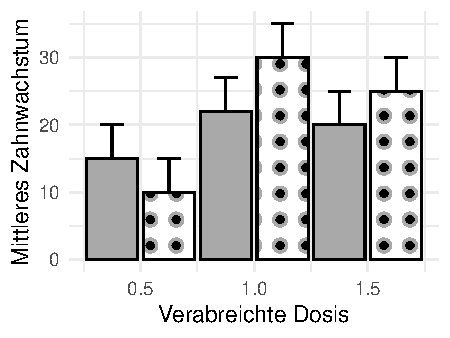
\includegraphics[width=\maxwidth]{img/mc-anova-02-a-1} 

}







\begin{enumerate}
\item [\textbf{A} \msquare] Eine mittlere bis starke Interaktion liegt vor $(p \leq 0.05)$
\item [\textbf{B} \msquare] Eine positive Interaktion liegt vor $(\rho \leq -0.5)$ 
\item [\textbf{C} \msquare] Eine Korrelation liegt vor $(p \leq 0.05)$.
\item [\textbf{D} \msquare] Keine Korrelation liegt vor $(p \geq 0.05)$.
\item [\textbf{E} \msquare] Keine Interaktion liegt vor $(p \leq 0.05)$.
\end{enumerate} 
\section*{Deskriptive Statistik \& Explorative Datenanalyse}

\section{Aufgabe \hfill (2 Punkte)}




Wie lautet der Mittelwert und Standardabweichung von $y$ mit 13, 8, 9, 11 und 13.



\begin{enumerate}
\item [\textbf{A} \msquare] Es berechnet sich 11.8 +/- 5.2
\item [\textbf{B} \msquare] Sie erhalten 10.8 +/- 1.14
\item [\textbf{C} \msquare] Es berechnet sich 10.8 +/- 5.2
\item [\textbf{D} \msquare] Sie erhalten 10.8 +/- 2.28
\item [\textbf{E} \msquare] Es ergibt sich 11.8 +/- 1.14
\end{enumerate} 

\section{Aufgabe \hfill (2 Punkte)}




Berechnen Sie den Median, das $1^{st}$ Quartile sowie das $3^{rd}$ Quartile von $y$ mit 28, 21, 25, 11, 27, 21, 12, 20, 25, 6 und 42.




\begin{enumerate}
\item [\textbf{A} \msquare] Es berechnet sich 22 [13; 26]
\item [\textbf{B} \msquare] Es ergibt sich 21 [12; 27]
\item [\textbf{C} \msquare] Sie erhalten 21 [10; 25]
\item [\textbf{D} \msquare] Es ergibt sich 22 +/- 12
\item [\textbf{E} \msquare] Sie erhalten 21 +/- 27
\end{enumerate} 

\section{Aufgabe \hfill (2 Punkte)}



Mit einem Histogramm  können Sie sehr gut die Verteilung von Daten visualisieren. Die empfohlene Mindestanzahl an Beobachtungen ist dabei?



\begin{enumerate}
\item [\textbf{A} \msquare] Wir sollten eine Beobachtung mindestens pro Gruppe vorliegen haben.
\item [\textbf{B} \msquare] Die opimale Anzahl ist größer als hundert Beobachtungen, wobei es gerne sehr viel mehr sein können.
\item [\textbf{C} \msquare] Die untere Grenze liegt bei zwei bis fünf Beobachtungen.
\item [\textbf{D} \msquare] 1 Beobachtung.
\item [\textbf{E} \msquare] Die untere Grenze liegt bei einer Beobachtung.
\end{enumerate}

\section{Aufgabe \hfill (2 Punkte)}



Die Varianz ist eine bedeutende deskriptive Statistik für die Analyse von Daten. Wie müssen Sie vorgehen um die Varianz zu berechnen?



\begin{enumerate}
\item [\textbf{A} \msquare] Als erstes berechnen wir den Mittelwert. Dann bilden wir die Summe der quadratischen Abstände zu dem Mittelwert. Abschließend teilen wir durch die Fallzahl.
\item [\textbf{B} \msquare] Den Mittelwert berechnen und die Abstände quadrieren. Die Summe mit der Fallzahl multiplizieren.
\item [\textbf{C} \msquare] Den Mittelwert berechen, dann die absoluten Abstände zum Mittelwert aufsummieren
\item [\textbf{D} \msquare] Als erstes berechnen wir den Mittelwert. Dann bilden wir die Summe der quadratischen Abstände zu dem Mittelwert. Abschließend subtrahieren wir die Fallzahl.
\item [\textbf{E} \msquare] Als erstes berechnen wir den Mittelwert. Dann bilden wir die Summe der quadratischen Abstände zu dem Mittelwert. Abschließend teilen wir durch die Fallzahl. Nicht zu vergessen, am Ende dann noch die Wurzel zu ziehen.
\end{enumerate} 

\section{Aufgabe \hfill (2 Punkte)}



In Ihrer Abschlußarbeit wolllen Sie Ihre Daten für den Ertrag in einem Boxplot darstellen. Sie nutzen den Boxplot auch, da der Boxplot zu den meist genutzten Visualiserungen von Daten gehört. Welche statistischen Maßzahlen stellt der Boxplot dar?

 



\begin{enumerate}
\item [\textbf{A} \msquare] Den Median und die Standardabweichung.
\item [\textbf{B} \msquare] Durch die Abbildung des Boxplot erhalten wir die Informationen über den Median und die Standardabweichung.
\item [\textbf{C} \msquare] Den Mittelwert sowie den Median und die Streuung.
\item [\textbf{D} \msquare] Den Mittelwert und die Standardabweichung.
\item [\textbf{E} \msquare] Durch die Abbildung des Boxplot erhalten wir die Informationen über den Median und die Quartile.
\end{enumerate}

\section{Aufgabe \hfill (2 Punkte)}



Nachdem Sie in einem Feldexperiment zu Leistungssteigerung von Brokoli durchgeführt haben, berechnen Sie den Mittelwert und den Median. Der Mittelwert $\bar{y}$ und der Median $\tilde{y}$ unterscheiden sich nicht. Welche Aussage ist richtig?



\begin{enumerate}
\item [\textbf{A} \msquare] Da sich der Mittelwert und der Median unterscheiden, ist der Datensatz nicht zu verwenden. Mittelwert und Median müssen gleich sein.
\item [\textbf{B} \msquare] Der Mittelwert und der Median sollten gleich sein, wenn keine Outlier in den Daten vorliegen. 
\item [\textbf{C} \msquare] Wenn sich der Mittelwert und der Median nicht unterscheiden, liegen vermutlich keine Outlier in den Daten vor.
\item [\textbf{D} \msquare] Wenn sich der Mittelwert und der Median nicht unterscheiden, liegen vermutlich Outlier in den Daten vor.
\item [\textbf{E} \msquare] Da sich der Mittelwert und der Median unterscheiden, liegen vermutlich keine Outlier in den Daten vor. Wir verweden den Datensatz so wie er ist.
\end{enumerate}

\section{Aufgabe \hfill (2 Punkte)}



Um zu Überprüfen, ob die Daten die Annahme einer Varianzhomogenität genügen, können wir folgende Visualisierung nutzen. Dabei kommt dann auch die entsprechende Regel zur Abschätzung der Annahme einer Varianzhomogenität zur Anwendung.



\begin{enumerate}
\item [\textbf{A} \msquare] In einer explorativen Datanalyse nutzen wir den Violinplot. Dabei sollte der Bauch am Rand liegen. Dann können wir von einer Varianzhomogenität ausgehen.
\item [\textbf{B} \msquare] Einen Dotplot. Die Punkte müssen sich wie an einer Perlenschnurr audreihen. Eine Abweichung führt zur Ablehnung der Annahme einer Varianzhomogenität.
\item [\textbf{C} \msquare] Wir erstellen uns für jede Behandlung einen Dotplot und schauen, ob die Dots und damit die Varianz für jede Behandlung gleich groß sind.
\item [\textbf{D} \msquare] Wir erstellen uns für jede Behandlung einen Boxplot und schauen, ob die Box und damit das IQR für jede Behandlung gleich groß ist.
\item [\textbf{E} \msquare] In einer explorativen Datanalyse nutzen wir den Boxplot. Dabei sollte der Median als dicke Linie in der Mitte der Box liegen. Dann können wir von einer Varianzhomogenität ausgehen.
\end{enumerate}

\section{Aufgabe \hfill (2 Punkte)}




Nach der Durchführung Ihres Feldexperiments wollen Sie eine ANOVA rechnen. Dafür muss aber Ihr Messwert zumindestens approximativ einer Normalverteilung folgen. Welche der drei Abbildungen erlaubt Ihnen abzuschätzen, ob Sie eine Normalverteilung in Ihrem Endpunkt vorliegen haben?





\begin{enumerate}
\item [\textbf{A} \msquare] Boxplot, Violinplot, Mosaicplot
\item [\textbf{B} \msquare] Boxplot, Densityplot, Violinplot
\item [\textbf{C} \msquare] Scatterplot, Densityplot, Barplot
\item [\textbf{D} \msquare] Violinplot, Scatterplot, Barplot
\item [\textbf{E} \msquare] Scatterplot, Mosaicplot, Boxplot
\end{enumerate} 

\section{Aufgabe \hfill (2 Punkte)}



Bevor Sie in Ihrer Abschlussarbeit einen statistischen Test rechnen, wollen Sie einmal betrachten, welcher Verteilung Ihre $n = 196$ geernteten Pflanzen folgen.  Welche Verteilung ist abgebildet?



{\centering 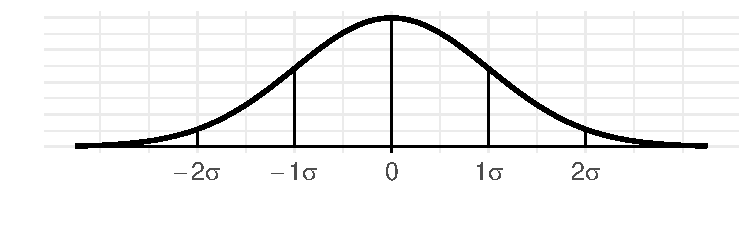
\includegraphics[width=\maxwidth]{img/mc-distribution-02-a-1} 

}







\begin{enumerate}
\item [\textbf{A} \msquare] Dem Histogramm entnehmen wir eine Possion-Verteilung.
\item [\textbf{B} \msquare] In dem Histogramm ist eine Ordinalverteilung dargestellt.
\item [\textbf{C} \msquare] Wir haben eine Gammaverteilung vorliegen.
\item [\textbf{D} \msquare] Eine Standardnormalverteilung.
\item [\textbf{E} \msquare] Wir haben eine Normalverteilung vorliegen.
\end{enumerate} 
\section*{Lineare Regression \& Korrelation}

\section{Aufgabe \hfill (2 Punkte)}



Im Allgemeinen gibt es zwei mögliche Ziele für ein Regressionsmodell. Wir können eine Vorhersagemodell oder ein kausales Modell rechnen. Welche Aussage ist für ein kausales Modell richtig?



\begin{enumerate}
\item [\textbf{A} \msquare] Ein kausales Modell benötigt mindestens eine Fallzahl von über 100 Beobachtungen und darf keine fehlenden Werte beinhalten. Die Varianzkomponenten müssen homogen sein.
\item [\textbf{B} \msquare] Ein kausales Modell basiert auf einem Traingsdatensatz und einem Testdatensatz. Auf dem Trainingsdatensatz wird das Modell trainiert und auf dem Testdatensatz validiert.
\item [\textbf{C} \msquare] Ein kausales Modell wird auf einem Trainingsdatensatz trainiert und anschliessend über eine explorative Datenanalyse validiert. Signifikanzen über $\beta_i$ können hier nicht festgestellt werden.
\item [\textbf{D} \msquare] Wir modellieren den Zusammenhang zwischen $X$ und $Y$ wenn ein kausales Modell rerechnet wird. Dabei kann der gesamte Datensatz genutzt werden. Eine Aufteilung wie in einem prädiktiven Modell ist nicht notwendig.
\item [\textbf{E} \msquare] Wenn ein kausales Modell gerechnet werden soll, dann muss zum einen ein Traingsdatensatz sowie ein Testdatensatz definiert werden. Dabei ist der Trainingsdatensatz meist 1/10 und der Testdatensatz 1/3 der Fallzahl groß. Der Testdatensatz dient zur Validierung.
\end{enumerate}

\section{Aufgabe \hfill (2 Punkte)}



Sie rechnen in eine linearen Regression und erhalten folgenden QQ Plot um die Annahme der normalverteilten Residuen zu überprüfen. Welche Aussage ist richtig?



{\centering 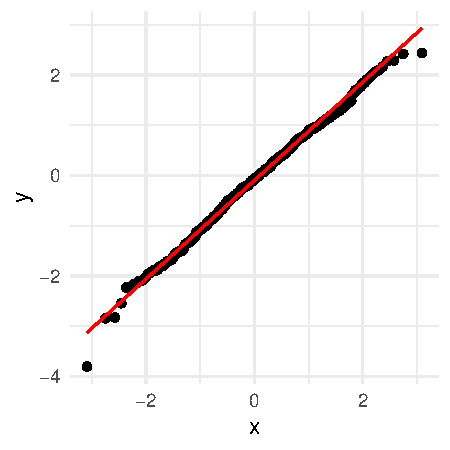
\includegraphics[width=\maxwidth]{img/mc-regression-05-a-1} 

}







\begin{enumerate}
\item [\textbf{A} \msquare] Wir betrachten die Gerade. Wenn die Punkte einigermaßen gleichmäßig um die Gerade verteilt liegen, dann gehen wir von normalverteilten Residuen aus. Dies ist hier nicht der Fall. Wir haben keine normalverteilten Residuen vorliegen.
\item [\textbf{B} \msquare] Wir betrachten die Gerade und dabei insbesondere die beiden Enden der Gerade. Hier sollten die Punkte auf der Geraden liegen, dann ist die Annahme an die Normalverteilung der Residuen erfüllt.
\item [\textbf{C} \msquare] Die Annahme der normalverteilten Residuen ist nicht erfüllt. Die Punkte liegen zum überwiegenden Teil auf der Geraden.
\item [\textbf{D} \msquare] Wir betrachten insbesondere die beiden Enden der Gerade. Der Rest ist mehr oder minder egal, dann ist die Annahme an die Normalverteilung der Residuen erfüllt.
\item [\textbf{E} \msquare] Wir betrachten die Punkte. Wenn die Punkte einigermaßen gleichmäßig verteilt liegen, dann gehen wir von normalen Residuen aus.
\end{enumerate}

\section{Aufgabe \hfill (2 Punkte)}



Nach einer Regressions sollten die Residuen (\texttt{.resid}) gleichmäßig um die Gerade verortet sein. Was bei einer simplen Regression noch relativ einfach visuell in einem Scatterplot zu überprüfen ist. Für komplexere Modell liefert der Residual Plot die notwendigen Informationen. Welche Aussage ist richtig?



{\centering 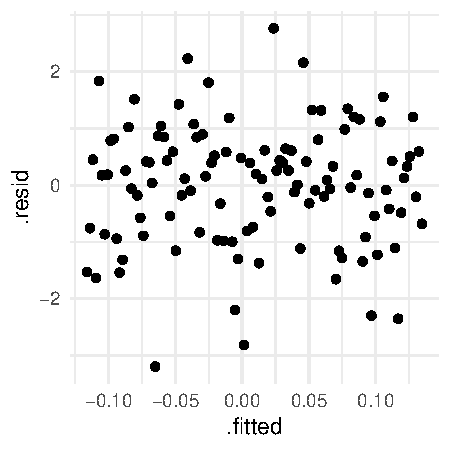
\includegraphics[width=\maxwidth]{img/mc-regression-06-a-1} 

}







\begin{enumerate}
\item [\textbf{A} \msquare] Wir betrachten die Nulllinie und alle Punkte sollten ohne Muster gleichmäßig um die Nulllinie liegen. Da dies der Fal ist, gehen wir von keinen Ausreißern aus.
\item [\textbf{B} \msquare] Wenn wir die Nulllinie betrachten so liegen die Punkte nicht gleichmäßig über und unter der Nulllinie. Unser Modell erfüllt nicht die Annahme von normalverteilten Residuen mit einem Mittelwert von 0 und einer Streuung von $s^2$.
\item [\textbf{C} \msquare] Die Annahme der normalverteilten Residuen ist erfüllt. Es ist ein Muster zu erkennen und wir können damit auf die Signifkanz von $x_1, ..., x_p$ schließen.
\item [\textbf{D} \msquare] Die Punkte müssen gleichmäßig in dem positiven Bereich liegen. Dies ist hier klar nicht der Fall. Einzelne Ausreißer können beobachtet werden. Die Analyse ist gescheitert.
\item [\textbf{E} \msquare] Die Annahme der normalverteilten Residuen ist nicht erfüllt. Es ist kein Muster zu erkennen.
\end{enumerate}

\section{Aufgabe \hfill (2 Punkte)}




In den Humanwissenschaften wird der Korrelationskoeffizienten $\rho$ sehr häufig verwendet. Daher ist es auch wichtig für andere Forschende den Korrelationskoeffizienten $\rho$ zu verstehen. Welche Aussazu zu dem Korrelationskoeffizienten $\rho$ ist richtig?




\begin{enumerate}
\item [\textbf{A} \msquare] Der Korrelationskoeffizienten $\rho$ ist eine veraltete Darstellungsform von Effekten in der linearen Regression und wird wie das $\eta^2$ aus der ANOVA interpretiert. Der Korrelationskoeffizienten $\rho$ beschreibt den Anteil an erklärter Varianz durch die Regression.
\item [\textbf{B} \msquare] Der Korrelationskoeffizienten $\rho$ wird wie das $\eta^2$ aus der ANOVA interpretiert. Der Korrelationskoeffizienten $\rho$ beschreibt den Anteil an erklärter Varianz durch die Regression. Dabei gibt er jedoch eine Richtung an und kann auch negativ werden.
\item [\textbf{C} \msquare] Korrelationskoeffizienten $\rho$ liegt zwischen 0 und 1. Darüber hinaus ist der Korrelationskoeffizienten $\rho$ einheitslos und kann als Standardisierung verstanden werden.
\item [\textbf{D} \msquare] Der Korrelationskoeffizienten $\rho$ liegt zwischen -1 und 1. Darüber hinaus ist der Korrelationskoeffizienten $\rho$ als standardisierte Steigung zu verstehen, wenn eine Standardisierung durchgeführt wurde. Diese Adjustierung nach Fischer muss am Anschluß der Berechnung der Korrelation durchgeführt werden.
\item [\textbf{E} \msquare] Der Korrelationskoeffizienten $\rho$ ist eine standardisierte, statistische Maßzahl, die zwischen -1 und 1 liegt. Dabei ist Korrelationskoeffizienten $\rho$ einheitslos.
\end{enumerate}

\section{Aufgabe \hfill (2 Punkte)}



Nach einer simplen linearen Regression zur Untersuchung vom Einfluss der $NO_3$-Konzentration in [$\mu g$] im Wasser auf das Wachstum von Brokkoli in [$kg$] erhalten Sie einen $\beta_{NO_3}$ Koeffizienten von $6.9\times 10^{-7}$ und einen hoch signifikanten $p$-Wert mit $0.00051$. Warum sehen Sie so einen kleinen Effekt bei einer so deutlichen Signifikanz?




\begin{enumerate}
\item [\textbf{A} \msquare] Manchmal ist die Einheit der Einflussvariable $X$ zu klein gewählt, so dass der Ansteig von 1 Einheit in $X$ zu einer zu kleinen Änderung in $y$ führt. Daher kann der Effekt $\beta_{NO_3}$ sehr klein wirken, aber auf einer anderen Einheit sehr viel größer sein. Der p-Wert wird auf einer einheitslosen Teststatistik bestimmt.
\item [\textbf{B} \msquare] Wenn der Effekt $\beta_{NO_3}$ winzig ist, dann kann es an einer falsch gewählten Einheit liegen. Der Anstieg von einer Einheit in $X$ führt ja zu einer Änderung von $\beta_{NO_3}$ in $x$. Wir müssen daher die Einheit von $y$ entsprechend anpassen.
\item [\textbf{C} \msquare] Das Gewicht und die $NO_3$-Konzentration korrelieren sehr stark, deshalb wird der $\beta_{NO_3}$ Koeffizient sehr klein. Mit einer ANOVA kann für die Korrelation korrigiert werden und der Effektschätzer passt dann zum p-Wert.
\item [\textbf{D} \msquare] Die Einheit der $NO_3$-Konzentration ist zu klein gewählt. Dadurch sehen wir den sehr kleinen $p$-Wert. Der $p$-Wert und die Einheit von der $NO_3$-Konzentration hängen antiproportional zusammen.
\item [\textbf{E} \msquare] Manchmal ist die Einheit der Einflussvariable $X$ zu groß gewählt, so dass der Ansteig von 1 Einheit in $X$ zu einer zu großen Änderung in $y$ führt. Daher kann der Effekt $\beta_{NO_3}$ sehr klein wirken, da der p-Wert wird auf einer einheitslosen Teststatistik bestimmt wird.
\end{enumerate}

\section{Aufgabe \hfill (2 Punkte)}



Nachdem Sie Ihr Experiment abgeschlossen haben, stehen Sie vor der Frage wie Sie Ihre Daten modellieren sollen. In der Beispielauswertung von Ihrem Betreuenden finden Sie die Funktion \texttt{lm()} in \Rlogo. Welche Aussage ist richtig?





\begin{enumerate}
\item [\textbf{A} \msquare] Ist die Einflussvariable $X$ numerisch so werden die Gruppenmittelwerte geschätzt und eine anschließende ANOVA sowie multipler Gruppenvergleich mit \{emmeans\} ist möglich.
\item [\textbf{B} \msquare] Die Funktion \texttt{lm()} in \Rlogo wird klassischerweise für die nicht-lineare Regression genutzt. Ist die Einflussvariable $X$ numerisch so werden die Gruppenmittelwerte geschätzt.
\item [\textbf{C} \msquare] Ist die Einflussvariable $X$ ein Faktor so werden die Gruppenmittelwerte geschätzt und eine anschließende ANOVA sowie multipler Gruppenvergleich mit \{emmeans\} ist möglich. Die Funktion \texttt{lm()} kann dabei eigentlich weggelassen werden, wird aber traditionell gerechnet.
\item [\textbf{D} \msquare] Ist die Einflussvariable $X$ ein Faktor so werden die Gruppenmittelwerte geschätzt und eine anschließende ANOVA sowie multipler Gruppenvergleich mit \{emmeans\} ist möglich. Dennoch muss zuerst ein lineares Modell mit der Funktion \texttt{lm()} in \Rlogo gerechnet werden.
\item [\textbf{E} \msquare] Die Funktion \texttt{lm()} in \Rlogo ist der letzte Schritt für einen Gruppenvergleich. Vorher kann eine ANOVA oder aber ein multipler Vergleich in \{emmeans\} gerechnet werden. In der Funktion  \texttt{lm()} werden die Gruppenvarianzen bestimmt.
\end{enumerate}

\section{Aufgabe \hfill (2 Punkte)}



Welche Aussage über das \textit{generalisierte lineare Modell (GLM)} ist richtig?




\begin{enumerate}
\item [\textbf{A} \msquare] Dank dem \textit{generalisierten linearen Modell (GLM)} können auch andere Verteilungsfamilien -- außer die Normalverteilung -- mit einer linearen Regression modelliert werden. Dafür werden alle Verteilungen in eine Normalverteilung überführt und anschließend standardisiert.
\item [\textbf{B} \msquare] Das GLM ist ein faktisch maschineller Lernalgorithmus, der selstständig die Verteilungsfamilie für Y wählt.
\item [\textbf{C} \msquare] Das GLM erlaubt auch nicht normalverteilte Residuen in der Schätzung der Regressionsgrade.
\item [\textbf{D} \msquare] Das \textit{generalisierte lineare Modell (GLM)} erlaubt auch weitere Verteilungsgruppen für das $X$ bzw. die Einflussvariablen in einer linearen Regression zu wählen.
\item [\textbf{E} \msquare] Das \textit{generalisierte lineare Modell (GLM)} erlaubt auch weitere Verteilungsfamilien für das $Y$ bzw. das Outcome in einer linearen Regression zu wählen.
\end{enumerate}
\section*{Vermischte Themen}  

\section{Aufgabe \hfill (2 Punkte)}

Die Randomisierung von Beobachtungen zu den Versuchseinheiten
ist bedeutend in der Versuchsplanung. Welche der folgenden Aussagen ist richtig?



\begin{enumerate}
\item [\textbf{A} \msquare] Randomisierung erlaubt erst die Mittelwerte zu schätzen. Ohne Randomisierung keine Mittelwerte. Ohne Mittelwerte keine Varianz und somit auch kein statistischer Test.
\item [\textbf{B} \msquare] Strukturgleichheit ist durch Randomisierung gegeben. Leider hilft die Randomisierung noch nicht um von der Stichprobe auf die Grundgesamtheit zu schließen. Deshalb wurde das Falsifikationsprinzip entwickelt.
\item [\textbf{C} \msquare] Strukturgleichheit ist durch Randomisierung gegeben. Somit kann von der Stichprobe auf die Grundgesamtheit geschlossen werden
\item [\textbf{D} \msquare] Randomisierung ist die direkte Folge von Strukturgleichheit. Die Strukturgleichheit erlaubt es erst von der Stichprobe auf die Grundgesamtheit zurückzuschliessen.
\item [\textbf{E} \msquare] Randomisierung erlaubt erst die Varianzen zu schätzen. Ohne eine Randomisierung ist die Berechnung von Mittelwerten und Varianzen nicht möglich. Dadurch lässt sich erst ein Experiment auswerten.
\end{enumerate}

\section{Aufgabe \hfill (2 Punkte)}



Wenn Sie einen Datensatz erstellen, dann ist es ratsam die Spalten und die Einträge in englischer Sprache zu verfassen, wenn Sie später die Daten in \Rlogo auswerten wollen. Welcher Aussage ist richtig?



\begin{enumerate}
\item [\textbf{A} \msquare] Im Allgemeinen haben Programmiersprachen Probleme mit Umlauten und Sonderzeichen, die in der deutschen Sprache vorkommen. Eine Nutzung der englischen Sprache umgeht dieses Problem auf einfache Art.
\item [\textbf{B} \msquare] \Rlogo Pakete sind nur in englischer Sprache verfasst. Es macht keinen Sinn \Rlogo daher in Deutsch zu bedienen.
\item [\textbf{C} \msquare] Die Spracherkennung von \Rlogo ist nicht in der Lage Deutsch zu verstehen.
\item [\textbf{D} \msquare] Es gibt keinen Grund nicht auch deutsche Wörter zu verwenden. Es ist ein Stilmittel.
\item [\textbf{E} \msquare] Alle Funktionen und auch Anwendungen sind in \Rlogo in englischer Sprache. Die Nutzung von deutschen Wörtern ist nicht schick und das ist zu vermeiden.
\end{enumerate}

\section{Aufgabe \hfill (2 Punkte)}



In Ihrer Abschlussarbeit wollen Sie zu Beginn eine explorativen Datenanalyse (EDA) in \Rlogo rechnen. Dafür gibt es eine generelle Abfolge von Prozessschritten. Welche ist hierbei die richtige Reihenfolge?



\begin{enumerate}
\item [\textbf{A} \msquare] Die Funktionsreihenfolge ist wie folgt: \texttt{read\_excel()} ->  \texttt{mutate()} -> \text{ggplot()}. Dabei ist bei der Transformation der Daten darauf zu achten, dass keine Faktoren erstellt werden.
\item [\textbf{B} \msquare] Wir lesen die Daten über eine generische Funktion \texttt{read()} ein und müssen dann die Funktion \texttt{ggplot()} nur noch installieren. Dann haben wir die Abbildungen als \texttt{*.png} vorliegen.
\item [\textbf{C} \msquare] Wir transformieren die Spalten über \texttt{mutate()} in ein \texttt{tibble} und können dann über \text{ggplot()} uns die Abbildungen erstellen lassen. Dabei beachten wir das wir keine Faktoren in den Daten haben.
\item [\textbf{D} \msquare] Wir lesen die Daten ein und mutieren die Daten. Dabei ist wichtig, dass wir nicht das Paket \texttt{tidyverse} nutzen, da dieses Paket veraltet ist. über die Funktion \texttt{library(tidyverse)} entfernen wir das Paket von der Analyse.
\item [\textbf{E} \msquare] Die Funktionsreihenfolge ist wie folgt: \texttt{read\_excel()} ->  \texttt{mutate()} -> \text{ggplot()}. Dabei ist bei der Transformation der Daten darauf zu achten, dass die Faktoren richtig erstellt werden.
\end{enumerate}

\section{Aufgabe \hfill (2 Punkte)}



Sie haben das abstrakte Modell $Y \sim X$ mit $X$ als Faktor mit zwei Leveln vorliegen. Welche Aussage über $n_1 < n_2$ ist richtig?



\begin{enumerate}
\item [\textbf{A} \msquare] Es liegt Varianzhetrogenität vor.
\item [\textbf{B} \msquare] Es handelt sich um ein balanciertes Design.
\item [\textbf{C} \msquare] Es handelt sich um unabhängige Beobachtungen.
\item [\textbf{D} \msquare] Es handelt sich um ein unbalanciertes Design.
\item [\textbf{E} \msquare] Es liegt Varianzhomogenität vor.
\end{enumerate}

\section{Aufgabe \hfill (2 Punkte)}



In einem Zuchtexperiment messen wir die Ferkel verschiedener Sauen. Die Ferkel einer Muttersau sind daher im statistischen Sinne...



\begin{enumerate}
\item [\textbf{A} \msquare] Die Ferkel stammen von der gleichen Sau und sind somit untereinander abhängig.
\item [\textbf{B} \msquare] Die Ferkel stammen von der gleichen Sau und sind somit untereinander unabhängig.
\item [\textbf{C} \msquare] Untereinander unabhängig. Sollten die Mütter verwandt sein, so ist die Varianzstruktur ähnlich und muss modelliert werden.
\item [\textbf{D} \msquare] Untereinander abhängig, wenn die Mütter ebenfalls miteinander verwandt sind. Erst die Abhängigkeit 2. Grades wird in der Statistik modelliert.
\item [\textbf{E} \msquare] Abhängig von der Stallanlage und des Experiments können die Ferkel abhängig oder unabhängig sein. Allgmein gilt, dass Ferkel von unterschiedlichen Sauen näher miteinander verwandt sind als Ferkel von gleichen Sauen. Das Fisher-Axiom.
\end{enumerate}

\section{Aufgabe \hfill (2 Punkte)}



In einer Studie wollen Sie den Effektschätzer Risk ratio berechnen. Sie finden in Ihrem Experiment zur Behandlung von Klaueninfektionen bei Ziegen in 3 Tieren Erkrankung der Klauen vor. 12 Tiere sind gesund. Welche Aussage ist richtig?



\begin{enumerate}
\item [\textbf{A} \msquare] Das Verhältnis der Chancen Risk ratio ergibt ein Chancenverhältnis von 0.2. Wir sind an der Chance krank zu sein interessiert.
\item [\textbf{B} \msquare] Der Anteil der Gesunden wird berechnet. Da es sich um ein Anteil handelt ergibt sich ein Risk ratio von 0.2.
\item [\textbf{C} \msquare] Da es sich um ein Chancenverhältnis handelt ergibt sich ein Risk ratio von 0.25.
\item [\textbf{D} \msquare] Es ergibt sich ein Risk ratio von 4, da es sich um ein Anteil handelt.
\item [\textbf{E} \msquare] Der Anteil der Kranken wird berechnet. Da es sich um ein Anteil handelt ergibt sich ein Risk ratio von 0.2.
\end{enumerate}

\section{Aufgabe \hfill (2 Punkte)}



Historisch gesehen ergibt sich ein Problem, wenn Sie mit sehr großen Datensätzen, wie in der Bio Data Sience üblich, rechnen. Warum ist es ein Problem, wenn Ihre Datensätze sehr groß werden hinsichtlich der Bewertung anhand der Signifikanz?




\begin{enumerate}
\item [\textbf{A} \msquare] Aktuell werden immer größere Datensätze erhoben. Eine erhöhte Fallzahl führt automatisch auch zu mehr signifikanten Ergebnissen, selbst wenn die eigentlichen Effekte nicht relevant sind.
\item [\textbf{B} \msquare] Riesige Datensätz haben mehr Fallzahl was zur $\alpha$-Inflation führt. Durch eine Adjustoerung kann dem Problem entgegengewirkt werden.
\item [\textbf{C} \msquare] Mehr Fallzahl in Datensätzen bedeutet mehr signifikante Ergebnisse, da in mehr Daten auch mehr Informationen beinhaltet sind. Deshalb lohnen sich riesige Datensätze, die durch die vielen signifikanten Ergebnisse auch eine Menge an relevanten Erkenntnissen liefern.
\item [\textbf{D} \msquare] Aktuell werden immer größere Datensätze erhoben. Dadurch wird auch die Varianz immer höher was automatisch zu mehr signifikanten Ergebnissen führt.
\item [\textbf{E} \msquare] Relevanz und Signifikanz haben nichts miteinander zu tun. Daher gibt es auch keinen Zusammenhang zwischen hoher Fahlzahl (n > 10000) und einem signifikanten Test. Ein Effekt ist immer relevant und somit signifikant.
\end{enumerate}
\section*{Multiple Gruppenvergleiche}    

\section{Aufgabe \hfill (2 Punkte)}



Sie haben folgende unadjustierten p-Werte gegeben: 0.89, 0.001, 0.03, 0.34 und 0.21. Sie adjustieren die p-Werte nach
Bonferroni. Welche Aussage ist richtig?



\begin{enumerate}
\item [\textbf{A} \msquare] Nach der Bonferroni-Adjustierung ergeben sich die adjustierten p-Werte von 4.45, 0.005, 0.15, 1.7 und 1.05. Die adjustierten p-Werte werden zu einem $\alpha$-Niveau von 5\% verglichen.
\item [\textbf{B} \msquare] Nach der Bonferroni-Adjustierung ergeben sich die adjustierten p-Werte von 0.178, 2e-04, 0.006, 0.068 und 0.042. Die adjustierten p-Werte werden zu einem $\alpha$-Niveau von 1\% verglichen.
\item [\textbf{C} \msquare] Nach der Bonferroni-Adjustierung ergeben sich die adjustierten p-Werte von 0.178, 2e-04, 0.006, 0.068 und 0.042. Die adjustierten p-Werte werden zu einem $\alpha$-Niveau von 5\% verglichen.
\item [\textbf{D} \msquare] Nach der Bonferroni-Adjustierung ergeben sich die adjustierten p-Werte von 1, 0.005, 0.15, 1 und 1. Die adjustierten p-Werte werden zu einem $\alpha$-Niveau von 5\% verglichen.
\item [\textbf{E} \msquare] Nach der Bonferroni-Adjustierung ergeben sich die adjustierten p-Werte von 1, 0.005, 0.15, 1 und 1. Die adjustierten p-Werte werden zu einem $\alpha$-Niveau von 1\% verglichen.
\end{enumerate}

\section{Aufgabe \hfill (2 Punkte)}



Sie rechnen einen PostHoc-Test. Nun sollen Sie ein \textit{CLD} erstellen. Was bedeutet dieser Fachbegriff und welche folgende Beschreibung der Interpretation ist korrekt?



\begin{enumerate}
\item [\textbf{A} \msquare] Compact letter display. Gleiche Buchstaben zeigen Gleichheit in den Behandlungen. Die Interpretation ist deshalb sehr intuitiv und einfach. Darüber hinaus ist damit das CLD auch auf einer Linie mit der Testtheorie, da wir ja auch dort die Gültigkeit der Nullhypothese nachweisen. Wir suchen ja Gleichheit.
\item [\textbf{B} \msquare] Compact letter display. Das CLD ist umstritten, da es die Gleichheit der Behandlungen durch gleiche Buchstaben darstellt. Dadurch ist das CLD nicht mehr sauber auf einer Linie mit dem statistischen Testen. Wir lehnen die Nullhypothese ab und zeigen keine Gleichheit im statistischen Testen.
\item [\textbf{C} \msquare] Compound letter display. Gleichheit in dem Outcomes wird durch den gleichen Buchstaben oder Symbol dargestellt. Teilweise ist die Interpretation des Verbunds (eng. compound) herausfordernd, da wir ja nach dem Unterschied suchen.
\item [\textbf{D} \msquare] Compact letter display. Gleiche Buchstaben bedeuten, dass sich die Behandlungen unterscheiden. Daher ist das CLD sehr unintuitiv. Es wäre besser, wenn gleiche Buchstaben Gleichheit anzeigen würden. Dies ist aber leider in der statistischen Testtheorie nicht möglich.
\item [\textbf{E} \msquare] Compact line display. Gleichheit in den Behandlungen wird durch den gleichen Buchstaben oder Symbol dargestellt. Früher wurden keine Buchstaben sondern eine durchgezogene Linie verwendet. Bei mehr als drei Gruppen funktioniert die Linie aber graphisch nicht mehr.
\end{enumerate}

\section{Aufgabe \hfill (2 Punkte)}




In Ihrer Bachelorarbeit müssen Sie einen Feldversuch auswerten. Nachdem Sie die zweifaktorielle ANOVA gerechnet haben und keine signifikante Interaktion vorliegt, wollen Sie jetzt einen Posthoc-Test rechnen. Welches R Paket nutzen Sie dafür am besten?



\begin{enumerate}
\item [\textbf{A} \msquare] Das R Paket \{hmisc\} erlaubt die Durchführung eines multiplen Gruppenvergleichs aus verschiedenen Modellen heraus. Aus einem hmisc Objekt lässt sich recht einfach das CLD erstellen und so über Barplots eine schnelle Interpration der statistischen Auswertung durchführen.
\item [\textbf{B} \msquare] Das R Paket \{lm\}. Das Paket \{lm\} erstellt selbstständig Konfidenzintervalle und entsprechende p-Werte. Da wir in dem Paket nicht adjustieren müssen, ist es bei Anwendern sehr beliebt.
\item [\textbf{C} \msquare] Das R Paket \{ggplot\}. Wir erhalten hier sofort eine Visualisierung der Daten. Anhand der Visualisierung lässt sich eine explorative Datenanalyse durchführen, die gleichwertig zu einem Posthoc-Test ist.
\item [\textbf{D} \msquare] Das R Paket \{emmeans\} erlaubt die Durchführung eines multiplen Gruppenvergleichs. Aus einem \{emmeans\} Objekt lässt sich recht einfach das CLD erstellen und so über Barplots eine schnelle Interpration der statistischen Auswertung durchführen.
\item [\textbf{E} \msquare] Das R Paket \{emmeans\} erlaubt die Durchführung eines multiplen Gruppenvergleichs. Aus einem emmeans Objekt lässt sich leider kein CLD erstellen. Dennoch ist das Paket einfach zu bedienen und wird deshalb genutzt. Die Interpretation der statistischen Auswertung wird über einen Barplot abgebildet.
\end{enumerate}

\section{Aufgabe \hfill (2 Punkte)}



Bei einem Posthoc-Test kann es zu einer überraschenden Besonderheit beim statistischen Testen kommen. Wie lautet der Fachbegriff und wie kann mit der überraschenden Besonderheit umgegangen werden?



\begin{enumerate}
\item [\textbf{A} \msquare] Beim multiplen Testen kann es zu einer $\alpha$-Inflation kommen. Das globale Signifikanzniveau liegt nicht mehr bei $5\%$ sondern weit darunter. Daher müssen die p-Werte entsprechend adjustiert werden. Hierfür gibt es verschiedene Verfahren, wobei das Verfahren zur Adjustierung der p-Werte nach Welch das bekanneste Verfahren ist.
\item [\textbf{B} \msquare] Das globale Signifikanzniveau liegt nicht mehr bei $5\%$ sondern sehr viel niedriger, bei ca. $1\%$. Es kommt zu einer $\alpha$-Hyperinflation. Dagegen kann mit der Adjustierung der p-Werte nach Bonferroni vorgegangen werden.
\item [\textbf{C} \msquare] Das globale Signifikanzniveau liegt nicht mehr bei $5\%$ sondern sehr viel höher. Es kommt zu einer $\alpha$-Inflation. Dagegen kann mit der Adjustierung der p-Werte nach Bonferroni vorgegangen werden.
\item [\textbf{D} \msquare] Beim multiplen Testen kann es zu einer $\beta$-Inflation kommen. Das globale Signifikanzniveau liegt nicht mehr bei $20\%$. Daher müssen die p-Werte entsprechend adjustiert werden. Hierfür gibt es verschiedene Verfahren, wobei das Verfahren zur Adjustierung der p-Werte nach Bonferroni das bekanneste Verfahren ist.
\item [\textbf{E} \msquare] Das globale Signifikanzniveau explodiert und erreicht Werte größer als Eins. Es kommt zu einer $\alpha$-Inflation. Dagegen kann mit der Adjustierung der $\alpha$-Werte nach Bonferroni vorgegangen werden.
\end{enumerate}

\section{Aufgabe \hfill (2 Punkte)}




Sie rechnen mehrere t-Tests für einen multiplen Vergleich nachdem eine einfaktorielle ANOVA sich als signifikant herausgestellt hat. Welche Aussage im Bezug auf den Effekt ist richtig? 



\begin{enumerate}
\item [\textbf{A} \msquare] Wenn ein multipler Test gerechnet wird, dann muss der Effekt $\Delta$ nicht adjustiert werden. Bei einem Effekt im multiplen Testen handelt es sich um eine Wahrscheinlichkeit für das Auftreten der Nullhypothese.
\item [\textbf{B} \msquare] Wenn ein multipler Test gerechnet wird, dann muss der Effekt $\Delta$ adjustiert werden im Gegensatz zu den p-Werten.
\item [\textbf{C} \msquare] Beim multiplen Testen kann es zu einer $\Delta$-Inflation kommen. Das globale Effektniveau liegt nicht mehr bei $20\%$. Daher müssen die Effekte entsprechend adjustiert werden. Hierfür gibt es verschiedene Verfahren, wobei das Verfahren zur Adjustierung der Effekte nach Bonferroni das bekanneste Verfahren ist.
\item [\textbf{D} \msquare] Beim multiplen Testen muss der Effekt, wie der Mittelwertsunterschied $\Delta$ aus einem t-Test, nicht adjusiert werden.
\item [\textbf{E} \msquare] Beim multiplen Testen kann es zu einer Effektüberschätzung ($\Delta$-Inflation) kommen. Daher müssen die Effekte angepasst werden. Dies geschieht nicht händisch sondern intern in den angewendeten Algorithmen.
\end{enumerate}
\section*{Statistische Testtheorie}  

\section{Aufgabe \hfill (2 Punkte)}




Sie haben den mathematischen Ausdruck $Pr(D|H_0)$ vorliegen, welche Aussage ist richtig?



\begin{enumerate}
\item [\textbf{A} \msquare] $Pr(D|H_0)$ stellt die Wahrscheinlichkeit die Daten $D$ und somit die Teststatistik $T_D$ zu beobachten dar, wenn die Nullhypothese wahr ist.
\item [\textbf{B} \msquare] $Pr(D|H_0)$ stellt die Wahrscheinlichkeit die Teststatistik $T$ zu beobachten dar, wenn die Nullhypothese falsch ist.
\item [\textbf{C} \msquare] Die Wahrscheinlichkeit der Daten unter der Nullhypothese in der Grundgesamtheit.
\item [\textbf{D} \msquare] $Pr(D|H_0)$ ist die Wahrscheinlichkeit nicht die Daten $D$ zu beobachten sondern die Nullhypothese, wenn diese wahr ist.
\item [\textbf{E} \msquare] $Pr(D|H_0)$ ist die Wahrscheinlichkeit der Alternativehypothese und somit $1 - Pr(H_A)$
\end{enumerate}

\section{Aufgabe \hfill (2 Punkte)}



Das statistische Testen basiert auf dem Falsifikationsprinzip. Es besagt,



\begin{enumerate}
\item [\textbf{A} \msquare] ... dass ein minderwertes Modell durch ein minderwertiges Modell ersetzt wird. Es gilt das Verifikationsprinzip nach Karl Popper.
\item [\textbf{B} \msquare] ... dass Annahmen an statistische Modelle meist falsch sind.
\item [\textbf{C} \msquare] ... dass ein minderwertes Modell durch ein weniger minderwertiges Modell ersetzt wird. Es gilt das Falsifikationsprinzip nach Karl Popper.
\item [\textbf{D} \msquare] ... dass ein schlechtes Modell durch ein schlechteres Modell ersetzt wird. Die Wissenschaft lehnt ab und verifiziert nicht.
\item [\textbf{E} \msquare] ... dass Fehlerterme in statistischen Modellen nicht verifiziert werden können.
\end{enumerate}

\section{Aufgabe \hfill (2 Punkte)}



In fast allen wissenschaftlichen Disziplinen liegt der Grenzwert für das Signifikanzniveau $\alpha$ bei 5\%. Wieso wurde dieser Konsens über die Signifikanzschwelle in dieser Form getroffen?



\begin{enumerate}
\item [\textbf{A} \msquare] Der Wert ergab sich aus einer Auswertung von 1042 wissenschaftlichen Veröffentlichungen zwischen 1914 und 1948. Der Wert $5\%$ wurde in $28\%$ der Veröffentlichungen genutzt. Daher legte man sich auf diese Zahl fest.
\item [\textbf{B} \msquare] Auf einer Statistikkonferenz in Genf im Jahre 1942 wurde dieser Cut-Off nach langen Diskussionen festgelegt. Bis heute ist der Cut Off aber umstritten, da wegen dem 2. Weltkrieg viele Wissenschaftler nicht teilnehmen konnten.
\item [\textbf{C} \msquare] In der Wissenschaft gibt es neben der Naturkonstante, die sich aus der Beobachtung der Welt ergibt, noch die Kulturkonstante, die von einer Gruppe Menschen selbstgewählt wird. Dabei ist $\alpha = 5\%$ eine Kulturkonstante und wurde somit eher zufällig gewählt.
\item [\textbf{D} \msquare] Da Wissenschaftler eine Schwelle für die statistische Testentscheidung benötigen wurde $\alpha$ in einer großen Konferenz 1945 gewählt. Damit ist $\alpha = 5\%$ eine Kulturkonstante mit einem Rank einer Naturkonstante.
\item [\textbf{E} \msquare] Als Kulturkonstante hat $\alpha = 5\%$ den Rang einer Naturkonstante und wurde nach langer Diskussion in der UN im Jahre 1983 festgesetzt. Damals auch schon mit der Zustimmung der UdSSR.
\end{enumerate}

\section{Aufgabe \hfill (2 Punkte)}

Betrachten wir die Teststatistik aus einem abstrakteren Blickwinkel. Beim
statistischen Testen wird das \textit{"`signal"'} mit dem
\textit{"`noise"'} aus den Daten $D$ zu einer Teststatistik $T_D$ verrechnet. Welche der Formel
berechnet korrekt die Teststatistik $T_D$?



\begin{enumerate}
\item [\textbf{A} \msquare] Es gilt $T_D = (signal \cdot noise)^2$
\item [\textbf{B} \msquare] Es gilt $T_D = signal \cdot noise$
\item [\textbf{C} \msquare] Es gilt $T_D = \cfrac{signal}{noise}$
\item [\textbf{D} \msquare] Es gilt $T_D = \cfrac{noise}{signal}$
\item [\textbf{E} \msquare] Es gilt $T_D = \cfrac{signal}{noise^2}$
\end{enumerate}

%% ------------------------------------------------------------

\section{Aufgabe \hfill (2 Punkte)}



Sie versuchen folgende Aussage richtig in die Analogie der statistischen Testtheorie zu setzen. Welche Analogie ist richtig?

\begin{center}
\textit{$H_0$ beibehalten obwohl die $H_0$ falsch ist}
\end{center}



\begin{enumerate}
\item [\textbf{A} \msquare] In die Analogie eines Feuerwehrautos: \textit{Car without noise}.
\item [\textbf{B} \msquare] Dem $\beta$-Fehler mit der Analogie eines brennenden Hauses: \textit{Fire without alarm}.
\item [\textbf{C} \msquare] Dem $\alpha$-Fehler in der Analogie eines Rauchmelder: \textit{Alarm without fire}.
\item [\textbf{D} \msquare] \textit{Fire without alarm}, dem $\beta$-Fehler als Analogie eines Rauchmelders.
\item [\textbf{E} \msquare] \textit{Fire without alarm}, dem $\beta$-Fehler als Analogie von Rauch im Haus.
\end{enumerate}

\section{Aufgabe \hfill (2 Punkte)}



Sie lesen eine wissenschaftliche Arbeit, die damit wirbt, dass Effekte und Signifikanz nicht separat dargestellt sind, sondern in einer statistischen Maßzahl zusammen. Welche Aussage ist richtig?



\begin{enumerate}
\item [\textbf{A} \msquare] Das Konfidenzintervall. Durch die Visualizierung des Konfidenzintervals kann eine Relevanzschwelle vom Anwender definiert werden. Zusätzlich erlaubt das Konfidenzinterval auch eine Entscheidung über die Signifikanz.
\item [\textbf{B} \msquare] Das OR. Als Chancenverhältnis gibt es das Verhältnis von Relevanz und Signifikanz wieder.
\item [\textbf{C} \msquare] Der p-Wert. Durch den Vergleich mit $\alpha$ lässt sich über die Signifikanz entscheiden und der $\beta$-Fehler erlaubt über die Power eine Einschätzung der Relevanz.
\item [\textbf{D} \msquare] Einem Konfidenzintervall. Das Konfidenzinterval bringt durch eine Visualisierung und drei Intervallgrenzen die Möglichkeit mit, eine Relevanzschwelle neben der Signifikanzschwelle und der $\alpha$-Schwelle zu definieren.
\item [\textbf{E} \msquare] Über das Konfidenzintervall. Das Konfidenzinterval inkludiert eine Entscheidung über die Relevanz und zusätzlich kann über die Visualizierung des Konfidenzintervals eine Signifikanzschwelle vom Forschenden definiert werden.
\end{enumerate}

\section{Aufgabe \hfill (2 Punkte)}



Welche Aussage über den $p$-Wert und dem Signifikanzniveau $\alpha$ gleich 5\% ist richtig?



\begin{enumerate}
\item [\textbf{A} \msquare] Wir vergleichen mit dem $p$-Wert und dem Signifikanzniveau $\alpha$ Wahrscheinlichkeiten und damit die absoluten Werte auf einem Zahlenstrahl, wenn die $H_0$ gilt.
\item [\textbf{B} \msquare] Wir machen eine Aussage über die indivduelle Wahrscheinlichkeit des Eintretens der Nullhypothese $H_0$. Der $p$-Wert wird mit dem Signifikanzniveau verglichen und bewertet.
\item [\textbf{C} \msquare] Wir vergleichen mit dem $p$-Wert und dem Signifikanzniveau $\alpha$ absolute Werte auf einem Zahlenstrahl und damit den Unterschied der Teststatistiken, wenn die $H_0$ gilt.
\item [\textbf{D} \msquare] Wir vergleichen die Effekte des $p$-Wertes mit den Effekten der Signifikanzschwelle unter der Annahme der Nullhypothese. Dabei gilt, dass wir die Nullhypothese nur ablehnen können anhand des Falsifikationsprinzips.
\item [\textbf{E} \msquare] Wir vergleichen mit dem $p$-Wert und dem Signifikanzniveau $\alpha$ Wahrscheinlichkeiten und damit die Flächen unter der Kurve der Teststatistik, wenn die $H_0$ gilt.
\end{enumerate}

\section{Aufgabe \hfill (2 Punkte)}



Die Ergebnisse der einer statistischen Analyse können in die Analogie einer Wettervorhersage gebracht werden. Welche Analogie für die Ergebnisse eines statistischen Tests trifft am besten zu?



\begin{enumerate}
\item [\textbf{A} \msquare] In der Analogie des Niederschlags oder Regenmenge: ein statistischer Test gibt die Stärke eines Effektes wieder. Zum Beispiel, wie hoch ist der Mittelwertsunterschied.
\item [\textbf{B} \msquare] In der Analogie der Maximaltemperatur: Was ist der maximale Unterschied zwischen zwei Gruppen. Wir erhalten hier eine Aussage über die Spannweite und den maximalen Effekt.
\item [\textbf{C} \msquare] In der Analogie der Durchschnittstemperatur: Wie oft tritt ein Effekt durchschnittlich ein? Wir erhalten eine Wahrscheinlichkeit für die Effekte. Zum Beispiel, wie hoch ist die Wahrscheinlichkeit für einen Mittelwert als Durchschnitt.
\item [\textbf{D} \msquare] In der Analogie der Wahrscheinlichkeit für Regen: ein statistischer Test erlaubt die Wahrscheinlichkeit für ein Ereignis abzuschätzen. Die Stärke des Effektes können wir nicht bestimmen.
\item [\textbf{E} \msquare] In der Analogie der Regenwahrscheinlichkeit in einem bestimmten Gebiet: ein statistischer Test gibt die Wahrscheinlichkeit für ein Ereignis in einem Experiment mit den Daten $D$ wieder und lässt sich kaum verallgemeinern.
\end{enumerate}

\section{Aufgabe \hfill (2 Punkte)}



In Ihrer Abschlussarbeit wollen Sie eine Aussage über ein untersuchtes Individuum treffen. Dazu nutzen Sie einen statistischen Test. Können Sie eine valide Aussage treffen?



\begin{enumerate}
\item [\textbf{A} \msquare] Ja, wir können ein untersuchtes Individuum nicht mit einem t-Test auswerten. Wir erhalten keine Aussage zum Individuum. Wir können aber den Effekt als Quelle der Relevanz nutzen.
\item [\textbf{B} \msquare] Ja, ein untersuchtes Individuum können wir mit einem statistischen Test auswerten. Wir erhalten dann eine Aussage zum Individuum.
\item [\textbf{C} \msquare] Nein, wir erhalten eine Aussage. Müssen aber das Individuum im Kontext der Population adjustieren.
\item [\textbf{D} \msquare] Nein, ein untersuchtes Individuum können wir mit einem statistischen Test nicht auswerten. Wir erhalten keine Aussage zum Individuum.
\item [\textbf{E} \msquare] Ja, wir erhalten nur eine Aussage zu zwei Individuen. Ein statistischer Test liefert Informationen zu einem Individuum im Vergleich zu einem anderen Individuum.
\end{enumerate}

\section{Aufgabe \hfill (2 Punkte)}



In der statistischen Testtheorie gibt es den Begriff \textit{Power}. Was sagt der statistische Begriff \textit{Power} aus?



\begin{enumerate}
\item [\textbf{A} \msquare] Die Power $1-\beta$ wird auf 80\% gesetzt. Alle statistischen Tests sind so konstruiert, dass die $H_A$ mit 80\% \textit{bewiesen wird}.
\item [\textbf{B} \msquare] Die Power ist nicht in der aktuellen Testthorie mehr vertreten. Wir rechnen nur noch mit dem Fehler 1. Art.
\item [\textbf{C} \msquare] Die Power beschreibt die Wahrscheinlichkeit die $H_A$ abzulehnen. Wir testen die Power jedoch nicht.
\item [\textbf{D} \msquare] Alle statistischen Tests sind so konstruiert, dass die $H_A$ mit 20\% \textit{bewiesen wird}. Die Power ist $1-\beta$ mit $\beta$ gleich 80\% gesetzt.
\item [\textbf{E} \msquare] Es gilt $\alpha + \beta = 1$ und somit liegt $\beta$ meist bei 95\%.
\end{enumerate}

\section{Aufgabe \hfill (2 Punkte)}



Sie rechnen einen statistischen Test und erhalten neben dem p-Wert noch einen Effekt wiedergegeben. Welche Aussage zum Effekt ist richtig?



\begin{enumerate}
\item [\textbf{A} \msquare] Der Effekt eines statistischen Tests beschreibt die mathematisch interpretierbare Ausgabe eines Tests. Damit ist der Effekt direkt mit dem Begriff der Signifikanz verbunden. Die Entscheidung über die Signifikanz trifft der Forschende unabhängig von der Relevanz eines statistsichen Tests.
\item [\textbf{B} \msquare] Durch den Effekt erfahren wir die statistische interpretierbare Ausgabe eines statistischen Tests. Zum Beispiel das $\eta^2$ aus einer ANOVA. Damit können wir die Signifikanz direkt mit dem Effekt verbinden. Am Ende muss der Forschende aber entscheiden, ob der Effekt entsprechend seinen Erwartungen als bedeutet zu bewerten ist.
\item [\textbf{C} \msquare] Der Effekt eines statistischen Tests beschreibt die biologisch interpretierbare Ausgabe eines Tests. Moderen Algorithmen liefern keine Effekte mehr sondern nur noch bedingte Wahrscheinlichkeiten. Der Effekt spielt in der modernen Statistik keine Rollen mehr.
\item [\textbf{D} \msquare] Der Effekt eines statistischen Tests beschreibt die biologisch interpretierbare Ausgabe eines Tests. Zum Beispiel den mittleren Unterschied zwischen zwei Gruppen aus einem t-Test. Damit ist der Effekt direkt mit dem Begriff der Relevanz verbunden. Die Entscheidung über die Relevanz trifft der Forschende unabhängig von der Signifikanz eines statistischen Tests.
\item [\textbf{E} \msquare] Der Effekt eines statistischen Tests beschreibt den Output oder die Wiedergabe eines Tests in einem Computer.
\end{enumerate}

\section{Aufgabe \hfill (2 Punkte)}



Welche Aussage über die Entscheidung anhand des p-Wertes gegen die
Nullhypothese ist richtig?



\begin{enumerate}
\item [\textbf{A} \msquare] Anhand des p-Wertes lässt sich wie folgt eine Entscheidung treffen. Liegt der Wert über oder gleich dem Signifikanzniveau $\alpha$ dann kann die Nullhypothese abgelehnt werden.
\item [\textbf{B} \msquare] Ist in dem 95\%-Konfidenzintervall nicht die Null enthalten dann wird die Nullhypothese $H_0$ abgelehnt.
\item [\textbf{C} \msquare] Ist $T_{D}$ h{"o}her als der kritische Wert $T_{\alpha = 5\%}$ dann wird die Nullhypothese $H_0$ abgelehnt.
\item [\textbf{D} \msquare] Anhand des p-Wertes lässt sich wie folgt eine Entscheidung treffen. Liegt der Wert in dem Signifikanzniveauintervall $\alpha$ dann kann die Nullhypothese abgelehnt werden.
\item [\textbf{E} \msquare] Ist $Pr(D|H_0)$ kleiner als das Signifikanzniveau $\alpha$ gleich $5\%$ dann wird die Nullhypothese $H_0$ abgelehnt.
\end{enumerate}

\section{Aufgabe \hfill (2 Punkte)}



Ein statistischer Test benötigt für die richtige Durchführung Hypothesen $H$, sonst ist der Test nicht zu interpretieren. Welche Aussage ist richtig?



\begin{enumerate}
\item [\textbf{A} \msquare] Es gibt ein Hypothesenset bestehend aus $k$ Hypothesen. Meistens wird die Nullhypothese $H_0$ und die Alternativhypothese $H_A$ verwendet. Wegen des Falsifikationsprinzips ist es wichtig, die bekannte falsche und unbekannte richtige Hypothese mit in das Set zu nehmen.
\item [\textbf{B} \msquare] Es gibt - bedingt durch das das Falsifikationsprinzip - ein Set von $k$ Nullhypothesen, die iterative gegen $k-1$ Alternativhypothesen getestet werden.
\item [\textbf{C} \msquare] Die Hypothesen $H_0$ und $H_A$ sind rein prosarischer Natur und bilden keinen mathematischen Hintergrund ab. In der Statistik wird die wissenschaftliche Fragestellung getestet. Daher stehen auch die verständlichen Hypothesen im Mittelpunkt der biologischen Interpretation.
\item [\textbf{D} \msquare] Es gibt ein statistisches Hypothesenpaar mit der Nullhypothese $H_0$ und der Alternativehypothese $H_A$ oder $H_1$.
\item [\textbf{E} \msquare] Mit der Nullhypothese $H_A$ und der Alternativehypothese $H_0$ gibt es zwei Hypothesen, die aber selten genutzt werden.
\end{enumerate}
\section*{Statistische Tests für Gruppenvergleiche} 

\section{Aufgabe \hfill (2 Punkte)}



Welche Aussage über den t-Test im Allgmeinen ist richtig? Berücksichtigen Sie den Welch t-Test wie auch den Student t-Test!



\begin{enumerate}
\item [\textbf{A} \msquare] Der t-Test vergleicht die Varianzen von mindestens zwei oder mehr Gruppen
\item [\textbf{B} \msquare] Der t-Test testet generell zu einem erhöhten $\alpha$-Niveau von 20\%.
\item [\textbf{C} \msquare] Der t-Test vergleicht zwei oder mehr Gruppen indem die Mittelwerte miteinander verglichen werden.
\item [\textbf{D} \msquare] Der t-Test ist ein Vortest der ANOVA und basiert daher auf dem Vergleich von Streuungsparametern
\item [\textbf{E} \msquare] Der t-Test vergleicht zwei Gruppen indem die Mittelwerte miteinander verglichen werden.
\end{enumerate}

\section{Aufgabe \hfill (2 Punkte)}



Die folgende Abbildung enthält die Daten aus einer Studie zur Bewertung der Wirkung des Mikronährstoff Sulfit auf den Ertrag in t/ha von Papaya im Vergleich zu einer Kontrolle. Der Versuch wurde in 8 Parzellen pro Gruppe durchgeführt. Welche Aussage im Bezug auf eine statistische Auswertung ist richtig?



{\centering 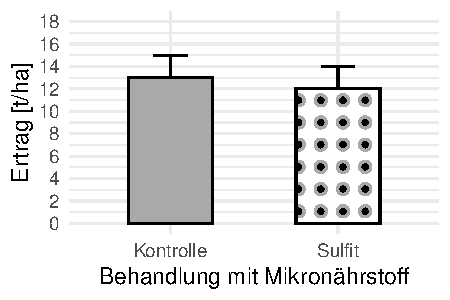
\includegraphics[width=\maxwidth]{img/mc-testing-ttest-02-1} 

}







\begin{enumerate}
\item [\textbf{A} \msquare] Der Test deutet auf ein signifikanten Unterschied hin. Der Effekt liegt vermutlich bei -8.
\item [\textbf{B} \msquare] Die Barplots deuten auf einen signifikanten Unterschied. Der Effekt liegt vermutlich bei -8. Wir müssen aber einen Posthoc-Test rechnen um den Effekt wirklich bestimmen zu können.
\item [\textbf{C} \msquare] Es liegt ein signifikanter Unterschied vor. Der Effekt liegt bei -0.8.
\item [\textbf{D} \msquare] Die Barplots deuten auf keinen signifikanten Unterschied. Der Effekt liegt vermutlich bei -8 unter einer groben Abschätzung. Wir müssen aber eine ANOVA rechnen um den Effekt wirklich bestimmen zu können.
\item [\textbf{E} \msquare] Der Test deutet auf keinen signifikanten Unterschied hin. Der Effekt liegt vermutlich bei -8.
\end{enumerate}

\section{Aufgabe \hfill (2 Punkte)}




Welche Aussage über den gepaarten t-Test für verbundene Stichproben ist richtig?



\begin{enumerate}
\item [\textbf{A} \msquare] Beim gepaarten t-Test kombinieren wir die Vorteile des Student t-Test für Varianzhomogenität mit den Vorteilen des Welch t-Test für Varianzheterogenität. Wir bilden dafür die Differenz der Einzelbeobachtungen.
\item [\textbf{B} \msquare] Der gepaarte t-Test wird gerechnet, wenn die Beobachtungen abhängig voneinander sind. Wir messen jede Beobachtung nur einmal und berechnen dann die Differenz zu dem Mittel der anderen Beobachtungen.
\item [\textbf{C} \msquare] Der gepaarte t-Test wird gerechnet, wenn die Beobachtungen nicht unabhängig voneinander sind. Wir messen wiederholt an dem gleichen Probanden oder Tier oder Pflanze. Wir bilden die Differenzen um den gepaarten t-Test rechnen zu können.
\item [\textbf{D} \msquare] Der gepaarte t-Test wird genutzt, wenn die Differenzen der Beobachtungen verbunden sind und wir dadurch die Unabhäängigkeit nicht mehr vorliegen haben.
\item [\textbf{E} \msquare] Der gepaarte t-Test nutzt die Varianz der Beobachtungen jeweils paarweise und bildet dafür eine verbundene Stichprobe. Dieser Datensatz $d$ dient dann zur Differenzbildung.
\end{enumerate}

\section{Aufgabe \hfill (2 Punkte)}



Nach einem Experiment mit drei Weizensorten ergibt eine ANOVA ($p = 0.048$) einen signifikanten Unterschied für den Ertrag. Sie führen anschließend die paarweisen t-Tests für alle Vergleiche der verschiedenen Weizensorten durch. Nach der Adjustierung für multiples Testen ist kein p-Wert unter der $\alpha$-Schwelle. Sie schauen sich auch die rohen, unadjustierten p-Werte an und finden hier als niedrigsten p-Wert $p_{3-2} = 0.053$. Welche Aussage ist richtig?




\begin{enumerate}
\item [\textbf{A} \msquare] Die ANOVA testet auf der gesamten Fallzahl. Es wäre besser die ANOVA auf der gleichen Fallzahl wie die einzelnen t-Tests zu rechnen.
\item [\textbf{B} \msquare] Hier kommt der Effekt der stiegenden Fallzahl auf die Anzahl an signifikante Ergebnisse zu tragen. Da die ANOVA auf weniger Fallzahl testet als die paarweisen t-Tests, kann die ANOVA schwerer einen signifikanten Unterscheid nachweisen.
\item [\textbf{C} \msquare] Die adjustierten p-Werte deuten in die richtige Richtung. Zusammen mit den nicht signifikanten rohen p-Werten ist von einem Fehler in der ANOVA auszugehen.
\item [\textbf{D} \msquare] Die ANOVA testet auf der gesamten Fallzahl. Die einzelnen t-Tests immer nur auf einer kleineren Subgruppe. Da mit weniger Fallzahl weniger signifikante Ergebnisse zu erwarten sind, kann eine Diskrepenz zwischen der ANOVA und den paarweisen t-Tests auftreten.
\item [\textbf{E} \msquare] Der Fehler liegt in den t-Tests. Wenn eine ANOVA signifikant ist, dann muss zwangsweise auch ein t-Test signifikant sein.
\end{enumerate}
    
% -----------------------------------------------------------------------
\clearpage
% -----------------------------------------------------------------------
\part{Deskriptive Statistik \& Explorative Datenanalyse}
% -----------------------------------------------------------------------

\section{Aufgabe \hfill (8 Punkte)}

\textit{Geben Sie grundsätzlich Formeln und Rechenweg zur Lösung der Teilaufgaben mit an!} \\[1Ex]
 

 
%% --------------------------------------------------------------------
\begin{minipage}[t]{0.5\textwidth}

\includegraphics[width = 1.3cm]{/Users/kruppajo/work/GitHub/exam/avatare/Yuki.png}
\end{minipage}
\begin{minipage}[t]{0.5\textwidth}
\hfill
\href{https://youtu.be/t0WYa_LVc5o}{
\includegraphics[width = 2cm]{img/youtube}}\\[1Ex]
\end{minipage}
\vspace{1ex}
%% --------------------------------------------------------------------



Anschauen, was andere vor einem gemacht haben, ist eine Möglichkeit schnell ans Ziel zu gelangen. Yuki soll in ihrem Projektbericht Kartoffeln untersuchen. Die Behandlung in ihrem Projektbericht werden verschiedene Lüftungssysteme und Folientunnel ($ctrl$, $storm$ und $tornado$) sein. Erheben wird Yuki als Endpunkt ($Y$) \textit{Ertrag} benannt als \textit{yield} in ihrer Exceldatei. Von ihrer Betreuerin erhält sie nun folgende Abbildung von Barplots, die sie erstmal zur Übung nachbauen soll, bevor sie mit dem eigentlichen Versuch beginnt.



{\centering 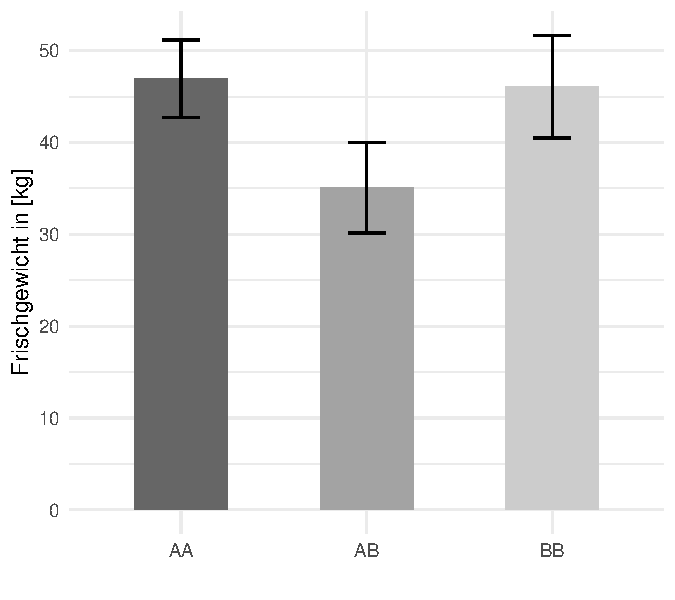
\includegraphics[width=\maxwidth]{img/barplot-02-1} 

}




Leider kennt sich Yuki mit der Erstellung von Barplots in \Rlogo nicht aus. Deshalb braucht sie bei der Visualisierung Ihre Hilfe!

\begin{enumerate}
\item Formulieren Sie die wissenschaftliche Fragestellung! \textbf{(1 Punkt)}
\item Erstellen Sie eine Tabelle mit den statistischen Maßzahlen aus der obigen Abbildung der drei Barplots! \textit{Beachten Sie die korrekte Darstellungsform der statistischen Maßzahlen!} \textbf{(3 Punkte)}
\item Erstellen Sie einen beispielhaften Datensatz, aus dem die drei Barplots \textit{möglicherweise} erstellt wurden, im \Rlogo üblichen Format! \textbf{(2 Punkte)}
\item Kann Yuki einen Unterschied zwischen den Behandlungen erwarten? Begründen Sie Ihre Antwort! \textbf{(2 Punkte)}
\end{enumerate} 
\clearpage
% -----------------------------------------------------------------------

\section{Aufgabe \hfill (8 Punkte)}

\textit{Geben Sie grundsätzlich Formeln und Rechenweg zur Lösung der Teilaufgaben mit an!} \\[1Ex]
 

 
%% --------------------------------------------------------------------
\begin{minipage}[t]{0.5\textwidth}

\includegraphics[width = 1.3cm]{/Users/kruppajo/work/GitHub/exam/avatare/Alex.png}
\end{minipage}
\begin{minipage}[t]{0.5\textwidth}
\hfill
\href{https://youtu.be/vXnLttRL_VI}{
\includegraphics[width = 2cm]{img/youtube}}\\[1Ex]
\end{minipage}
\vspace{1ex}
%% --------------------------------------------------------------------



Alex steht vor einem ersten Problem, denn wenn es nach seinem Betreuer geht, soll er in einem einer Klimakammer Erbsen auswertet. Soweit eigentlich alles passend. Die Behandlung waren verschiedene Lichtstufen ($none$, $200lm$ und $600lm$). In seiner Exceldatei hat er den Outcome ($Y$) \textit{Frischegewicht} als \textit{freshmatter} aufgenommen. Nun soll Alex die Daten eimal als Barplots in einer Präsentation visualisieren, damit seinem Betreuer wieder klar wird, was er eigentlich nochmal gemacht hat und was für ein Ergbnis in einem statistischen Test zu erwarten wäre.

\begin{table}[!h]
\centering
\begin{tabular}{cc}
\toprule
treatment & freshmatter\\
\midrule
200lm & 41.7\\
600lm & 31.2\\
none & 37.9\\
200lm & 41.1\\
none & 24.8\\
\addlinespace
none & 21.6\\
200lm & 39.1\\
600lm & 40.1\\
600lm & 41.0\\
600lm & 28.8\\
\addlinespace
600lm & 30.4\\
\bottomrule
\end{tabular}
\end{table}



Leider kennt sich Alex mit der Erstellung von Barplots nicht aus. Deshalb braucht er bei der Visualisierung Ihre Hilfe!

\begin{enumerate}
\item Formulieren Sie die wissenschaftliche Fragestellung! \textbf{(1 Punkt)}
\item Zeichnen Sie in \textit{einer} Abbildung die Barplots für die Behandlung von Erbsen! Beschriften Sie die Achsen entsprechend!\textbf{(4 Punkte)}
\item Beschriften Sie \textit{einen} Barplot mit den gängigen statistischen Maßzahlen! \textbf{(2 Punkte)}
\item Wenn Alex \textit{keinen Effekt} zwischen den Behandlungen von Erbsen erwarten würde, wie sehen dann die Barplots aus? \textit{Antworten Sie mit einer Skizze der Barplots!}
  \textbf{(1 Punkt)}
\end{enumerate} 
\clearpage
% -----------------------------------------------------------------------

\section{Aufgabe \hfill (9 Punkte)}

\textit{Geben Sie grundsätzlich Formeln und Rechenweg zur Lösung der Teilaufgaben mit an!} \\[1Ex]
 

 
%% --------------------------------------------------------------------
\begin{minipage}[t]{0.5\textwidth}

\includegraphics[width = 1.3cm]{/Users/kruppajo/work/GitHub/exam/avatare/Nilufar.png}
\end{minipage}
\begin{minipage}[t]{0.5\textwidth}
\hfill
\href{https://youtu.be/Xf0yE-o7bEU}{
\includegraphics[width = 2cm]{img/youtube}}\\[1Ex]
\end{minipage}
\vspace{1ex}
%% --------------------------------------------------------------------



Anschauen, was andere vor einem gemacht haben, ist eine Möglichkeit schnell ans Ziel zu gelangen. Nilufar soll in ihrer Abschlussarbeit Brokoli untersuchen. Die Behandlung in ihrer Abschlussarbeit werden verschiedene Bewässerungstypen ($low$, $mid$ und $high$) sein. Erheben wird Nilufar als Outcome ($Y$) \textit{Trockengewicht} benannt als \textit{drymatter} in ihrer Exceldatei. Von ihrem Betreuer erhält sie nun folgende Abbildung von Boxplots, die sie erstmal zur Übung nachbauen soll, bevor sie mit dem eigentlichen Versuch beginnt. Anhand von Boxplots lässt sich eine Aussage über die Normalverteilung von $Y$ treffen.



{\centering 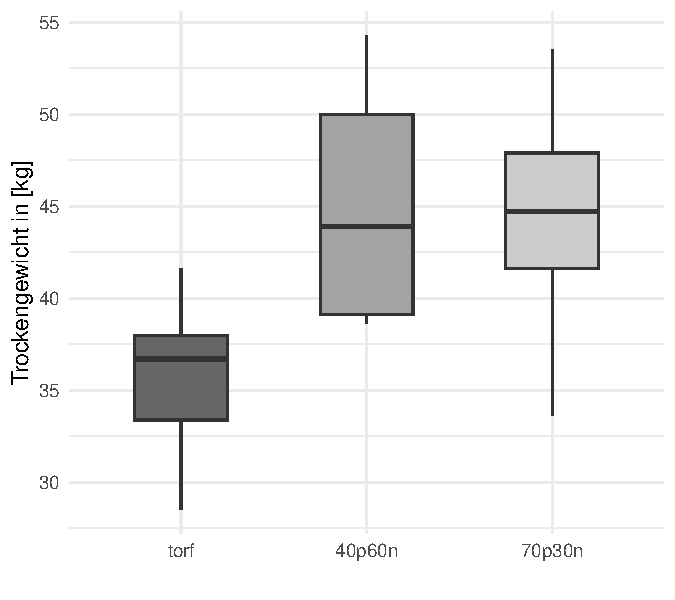
\includegraphics[width=\maxwidth]{img/boxplot-02-zer-1} 

}




Leider kennt sich Nilufar mit der Erstellung von Boxplots in \Rlogo nicht aus. Deshalb braucht sie bei der Visualisierung Ihre Hilfe!

\begin{enumerate}
\item Erstellen Sie eine Tabelle mit den statistischen Maßzahlen aus der obigen Abbildung der drei Boxplots! \textit{Beachten Sie die korrekte Darstellungsform der statistischen Maßzahlen!} \textbf{(3 Punkte)}
\item Beschriften Sie \textit{einen} der Boxplots mit den gängigen statistischen Maßzahlen! \textbf{(2 Punkte)}
\item Erstellen Sie einen beispielhaften Datensatz, aus dem die drei Boxplots \textit{möglicherweise} erstellt wurden, im \Rlogo üblichen Format! \textbf{(2 Punkte)}
\item Kann Nilufar einen Unterschied zwischen den Behandlungen erwarten? Begründen Sie Ihre Antwort! \textbf{(2 Punkte)}
\end{enumerate} 
\clearpage
% -----------------------------------------------------------------------

\section{Aufgabe \hfill (9 Punkte)}

\textit{Geben Sie grundsätzlich Formeln und Rechenweg zur Lösung der Teilaufgaben mit an!} \\[1Ex]
 

 
%% --------------------------------------------------------------------
\begin{minipage}[t]{0.5\textwidth}

\includegraphics[width = 1.3cm]{/Users/kruppajo/work/GitHub/exam/avatare/Jessica.png}
\end{minipage}
\begin{minipage}[t]{0.5\textwidth}
\hfill
\href{https://youtu.be/0xc0jIPeiyw}{
\includegraphics[width = 2cm]{img/youtube}}\\[1Ex]
\end{minipage}
\vspace{1ex}
%% --------------------------------------------------------------------



Jessica steht vor einem ersten Problem, denn wenn es nach ihrem Betreuer geht, soll sie in einem einem Gewächshausexperiment Kartoffeln auswertet. Soweit eigentlich alles passend. Die Behandlung waren verschiedene Düngestufen ($ctrl$ und $high$). In ihrer Exceldatei hat sie den Messwert ($Y$) \textit{Proteingehalt} als \textit{protein} aufgenommen. Nun soll Jessica die Daten eimal als Boxplots in einer Präsentation visualisieren, damit ihrem Betreuer wieder klar wird, was sie eigentlich nochmal gemacht hat und was für ein Ergbnis in einem statistischen Test zu erwarten wäre. Anhand von Boxplots lässt sich eine Aussage über die Varianzhomogenität über die Behandlungsgruppen treffen.

\begin{table}[!h]
\centering
\begin{tabular}{cc}
\toprule
treatment & drymatter\\
\midrule
high & 47.2\\
high & 50.0\\
high & 36.5\\
high & 47.8\\
high & 36.1\\
\addlinespace
high & 47.0\\
ctrl & 21.0\\
high & 33.0\\
ctrl & 21.8\\
high & 41.7\\
\addlinespace
ctrl & 20.5\\
ctrl & 19.5\\
ctrl & 11.0\\
ctrl & 14.5\\
ctrl & 9.9\\
\addlinespace
ctrl & 20.2\\
ctrl & 30.3\\
\bottomrule
\end{tabular}
\end{table}



Leider kennt sich Jessica mit der Erstellung von Boxplots nicht aus. Deshalb braucht sie bei der Visualisierung Ihre Hilfe!

\begin{enumerate}
\item Zeichnen Sie in \textit{einer} Abbildung die beiden Boxplots für die zwei Behandlungen von Kartoffeln! Beschriften Sie die Achsen entsprechend! \textbf{(5 Punkte)} 
\item Wie ist Ihr Vorgehen, wenn Sie eine \textit{gerade} Anzahl an
  Beobachtungen pro Gruppe haben? \textbf{(1 Punkt)}
\item Beschriften Sie \textit{einen} der beiden Boxplots mit den gängigen
  statistischen Maßzahlen! \textbf{(2 Punkte)}
\item Wenn Sie \textit{keinen Effekt} zwischen den Behandlungen von
  Kartoffeln erwarten würden, wie sehen dann die beiden Boxplots aus?
  \textit{Antworten Sie mit einer Skizze der Boxplots!}
  \textbf{(1 Punkt)}
\end{enumerate} 
\clearpage
% -----------------------------------------------------------------------

\section{Aufgabe \hfill (8 Punkte)}

\textit{Geben Sie grundsätzlich Formeln und Rechenweg zur Lösung der Teilaufgaben mit an!} \\[1Ex]
 

 
%% --------------------------------------------------------------------
\begin{minipage}[t]{0.5\textwidth}

\includegraphics[width = 1.3cm]{/Users/kruppajo/work/GitHub/exam/avatare/Yuki.png}
\end{minipage}
\begin{minipage}[t]{0.5\textwidth}
\hfill
\href{https://youtu.be/aXvxGC4YLqk}{
\includegraphics[width = 2cm]{img/youtube}}\\[1Ex]
\end{minipage}
\vspace{1ex}
%% --------------------------------------------------------------------



Yuki betrachtet die folgenden Daten nach einem Freilandversuch mit Kartoffeln. In dem Experiment wurden die seltsamen Verdickungen gezählt. Nach der Meinung seinem Betreuer muss als erstes geschaut werden, wie diese verteilt sind. Also welcher statistischen Verteilung die seltsamen Verdickungen folgen. Dazu soll Yuki ein Histogramm verwenden. Dann hätte man auch einen guten Überblick über den Messwert ($Y$).

\begin{center}
Die seltsamen Verdickungen: 4, 4, 7, 3, 6, 7, 4, 3, 5, 10, 1, 2, 5, 1, 5, 4, 6, 2, 2, 2, 4, 1, 5, 2, 3, 2, 7, 7, 4, 4, 6, 5, 6, 4, 3, 4
\end{center}

Leider kennt sich Yuki mit der Erstellung von Histogrammen überhaupt nicht aus. Deshalb braucht er bei der Erstellung Ihre Hilfe!

\begin{enumerate}
\item Zeichen Sie ein Histogramm um die Verteilung der Daten zu visualisieren! (\textbf{3 Punkte})
\item Beschriften Sie die Achsen der Abbildung! (\textbf{2 Punkte})
\item Ergänzen Sie die absoluten und relativen Häufigkeiten in der
  Abbildung! \textbf{(1 Punkt)}
\item Berechnen Sie aus den Daten die \textit{Wahrscheinlichkeit}
  mehr als die Anzahl 4 zu beobachten! \textbf{(1
    Punkt)}
\item Berechnen Sie aus den Daten die \textit{Chance} mehr
  als die Anzahl 4 zu beobachten! \textbf{(1 Punkt)}
\end{enumerate}

 
\clearpage
% -----------------------------------------------------------------------

\section{Aufgabe \hfill (8 Punkte)}

\textit{Geben Sie grundsätzlich Formeln und Rechenweg zur Lösung der Teilaufgaben mit an!} \\[1Ex]
 

 
%% --------------------------------------------------------------------
\begin{minipage}[t]{0.5\textwidth}

\includegraphics[width = 1.3cm]{/Users/kruppajo/work/GitHub/exam/avatare/Jessica.png}
\end{minipage}
\begin{minipage}[t]{0.5\textwidth}
\hfill
\href{https://youtu.be/ORHSPTCdfeY}{
\includegraphics[width = 2cm]{img/youtube}}\\[1Ex]
\end{minipage}
\vspace{1ex}
%% --------------------------------------------------------------------



Jessica betrachtet die folgenden Daten nach einem Versuch in einer Klimakammer mit Kartoffeln. In dem Experiment wurden die mittleren Mehltauspots gezählt. Nach der Meinung ihrer Betreuerin muss als erstes geschaut werden, wie diese verteilt sind. Also welcher statistischen Verteilung die mittleren Mehltauspots folgen. Dazu soll Jessica ein Histogramm verwenden. Dann hätte man auch einen guten Überblick über den Messwert ($Y$).

\begin{center}
Die mittleren Mehltauspots: 15.1, 11.9, 11.8, 12.3, 8.4, 9.2, 9.9, 9.3, 11, 9.6, 10.5, 7.4, 6.5, 16.4, 9.8, 8.8, 15.4, 13.3, 12, 9.3, 8.6, 12.3
\end{center}

Leider kennt sich Jessica mit der Erstellung von Histogrammen überhaupt nicht aus. Deshalb braucht sie bei der Erstellung Ihre Hilfe!

\begin{enumerate}
\item Zeichen Sie ein Histogramm um die Verteilung der Daten zu
  visualisieren! (\textbf{3 Punkte})
 \item Erläutern Sie Ihr Vorgehen um ein Histogramm für kontinuierliche
  Daten zu zeichnen!  (\textbf{2 Punkte})
\item Beschriften Sie die Achsen der Abbildung! (\textbf{2 Punkte})
\item Ergänzen Sie die relativen Häufigkeiten in der Abbildung! \textbf{(1
    Punkt)}  
\end{enumerate}

 
\clearpage
% -----------------------------------------------------------------------

\section{Aufgabe \hfill (10 Punkte)}

\textit{Geben Sie grundsätzlich Formeln und Rechenweg zur Lösung der Teilaufgaben mit an!} \\[1Ex]
 

 
%% --------------------------------------------------------------------
\begin{minipage}[t]{0.5\textwidth}

\includegraphics[width = 1.3cm]{/Users/kruppajo/work/GitHub/exam/avatare/Nilufar.png}
\end{minipage}
\begin{minipage}[t]{0.5\textwidth}
\hfill
\href{https://youtu.be/VAqiUdV4WQ0}{
\includegraphics[width = 2cm]{img/youtube}}\\[1Ex]
\end{minipage}
\vspace{1ex}
%% --------------------------------------------------------------------




Nilufar möchte gerne den Zusammenhang zwischen durchschnittliche UV Einstrahlung [UV/d] und Proteingehalt [g/kg] im Kontext von Kartoffeln herausfinden. Hierfür hat Nilufar ein Gewächshausexperiment im Wendland durchgeführt. Nach einigen unvorgesehenen Ereignissen hat sie es geschafft folgende Datentabelle zu erstellen. Nun stellt sich die Frage für sie, ob es überhaupt einen Zusammenhang zwischen den gemessenen Variablen gibt. Deshalb möchte Nilufar als erstes eine explorative Datenanalyse durchführen.

\begin{table}[!h]
\centering
\begin{tabular}{cc}
\toprule
Proteingehalt [g/kg] & Durchschnittliche UV Einstrahlung [UV/d]\\
\midrule
25.7 & 36.9\\
27.6 & 39.3\\
27.8 & 41.8\\
22.7 & 35.9\\
22.4 & 35.5\\
\addlinespace
24.6 & 34.9\\
28.6 & 40.4\\
22.7 & 31.2\\
22.3 & 26.6\\
\bottomrule
\end{tabular}
\end{table}



Leider kennt sich Nilufar mit der Erstellung einer explorativen Datenanalyse für kontinuierliche Daten überhaupt nicht aus. Deshalb braucht sie bei der Erstellung Ihre Hilfe!

\begin{enumerate}
\item Erstellen Sie eine Visualisierung für die Datentabelle. Beschriften Sie
  die Achsen entsprechend! \textbf{(4 Punkte)}
\item Schätzen Sie eine Gerade durch die Punkte! \textbf{(1 Punkt)}
\item Beschriften Sie die Gerade mit den gängigen statistischen Maßzahlen! Geben Sie die numerischen Zahlenwerte mit an! \textbf{(3 Punkte)}
\item Wenn \textit{ein} Effekt von $x$ auf $y$ vorhanden wäre, wie würde die Gerade verlaufen und welche Werte würden die statistischen Maßzahlen annehmen? \textbf{(2 Punkt)}
\end{enumerate} 
\clearpage
% -----------------------------------------------------------------------

\section{Aufgabe \hfill (10 Punkte)}

\textit{Geben Sie grundsätzlich Formeln und Rechenweg zur Lösung der Teilaufgaben mit an!} \\[1Ex]
 

 
%% --------------------------------------------------------------------
\begin{minipage}[t]{0.5\textwidth}

\includegraphics[width = 1.3cm]{/Users/kruppajo/work/GitHub/exam/avatare/Jonas.png}
\end{minipage}
\begin{minipage}[t]{0.5\textwidth}
\hfill
\href{https://youtu.be/t_1KL77mfmg}{
\includegraphics[width = 2cm]{img/youtube}}\\[1Ex]
\end{minipage}
\vspace{1ex}
%% --------------------------------------------------------------------



'Uff!', denkt sich Jonas. Jetzt hat er doch tatsächlich zwei kategoriale Variablen in seinem Projektbericht gemessen. Zum einen die Behandlung Herbizideinsatz [ja/nein] und zum anderen die Messung Proteingehalt im Zielbereich [ja/nein] im Kontext von Kartoffeln. Hierfür hat er ein Gewächshausexperiment im Emsland durchgeführt. Jetzt möchte Jonas die Daten einmal in einer explorativen Datenanalyse darstellen. Danach kann er dann über den passenden statistischen Test nachdenken. Dabei unterstützt seine Betreuerin diesen Ansatz bevor es in der Datenanalyse weiter geht.



\vspace{1Ex}

\begin{center}
\begin{minipage}[t]{0.45\textwidth}
\small
\begin{center}

\begin{tabular}{p{2.5cm}p{2.5cm}p{2.5cm}p{2.5cm}}
\toprule
Herbizideinsatz & Proteingehalt im Zielbereich\\
\midrule
ja & nein\\
ja & ja\\
ja & ja\\
nein & ja\\
nein & nein\\
\addlinespace
ja & nein\\
ja & ja\\
ja & nein\\
ja & nein\\
nein & nein\\
\addlinespace
ja & ja\\
ja & ja\\
nein & ja\\
nein & ja\\
ja & nein\\
\addlinespace
ja & ja\\
\bottomrule
\end{tabular}


\end{center}
\end{minipage}
\begin{minipage}[t]{0.45\textwidth}
\small
\begin{center}

\begin{tabular}{p{2.5cm}p{2.5cm}p{2.5cm}p{2.5cm}}
\toprule
Herbizideinsatz & Proteingehalt im Zielbereich\\
\midrule
nein & nein\\
ja & ja\\
ja & ja\\
nein & nein\\
nein & nein\\
\addlinespace
nein & ja\\
nein & ja\\
ja & ja\\
nein & nein\\
nein & nein\\
\addlinespace
nein & ja\\
ja & ja\\
ja & nein\\
ja & ja\\
ja & ja\\
\addlinespace
nein & ja\\
\bottomrule
\end{tabular}


\end{center}
\end{minipage}
\end{center}

\vspace{2Ex}

Leider kennt sich Jonas mit der Erstellung einer explorativen Datenanalyse für kategoriale Daten überhaupt nicht aus. Deshalb braucht er bei der Erstellung Ihre Hilfe!

\begin{enumerate}
\item Stellen Sie den Zusammenhang zwischen den beiden kategorialen Variablen in einer zusammenfassenden Tabelle dar! \textbf{(3 Punkte)}
\item Visualisieren Sie den Zusammenhang zwischen den beiden kategorialen Variablen! \textbf{(3 Punkte)}
\item Berechnen Sie die Verhältnisse in der Visualisierung! Welche Annahme haben Sie getroffen? \textbf{(2 Punkte)}
\item Wenn \textit{ein} Effekt von der Behandlung vorliegen würde, wie würde die Tabelle und die Visualisierung aussehen? \textbf{(2 Punkt)}
\end{enumerate} 
\clearpage
% -----------------------------------------------------------------------

\section{Aufgabe \hfill (10 Punkte)}

\textit{Geben Sie grunds{\"a}tzlich Formeln und Rechenweg zur L{\"o}sung der
  Teilaufgaben mit an!} \\[1Ex]

%% --------------------------------------------------------------------
\hfill\href{https://youtu.be/Op-gjzASH9I}{
\includegraphics[width =
  2cm]{img/youtube}}\\[1Ex]
%% --------------------------------------------------------------------



\begin{enumerate}
\item Zeichnen Sie {\"u}ber die untenstehenden Boxplots die entsprechende
  zugeh{\"o}rige Verteilung! \textbf{(3 Punkte)} 
\item Zeichnen Sie unter die untenstehenden Boxplots die entsprechende
  zugeh{\"o}rige Beobachtungen als Stiche! \textbf{(3 Punkte)}
\item Wieviel Prozent der Beobachtungen fallen in das IQR? Erg{\"a}nzen Sie die
  Abbildung entsprechend um den Bereich! \textbf{(2 Punkte)}
\item Wieviel Prozent der Beobachtungen fallen in $\pm 2s$ unter
  der Annahme einer Normalverteilung?  \textit{Wenn m{\"o}glich}, erg{\"a}nzen Sie
  die Abbildung entsprechend um den Bereich! \textbf{(2 Punkte)}
\end{enumerate}




{\centering 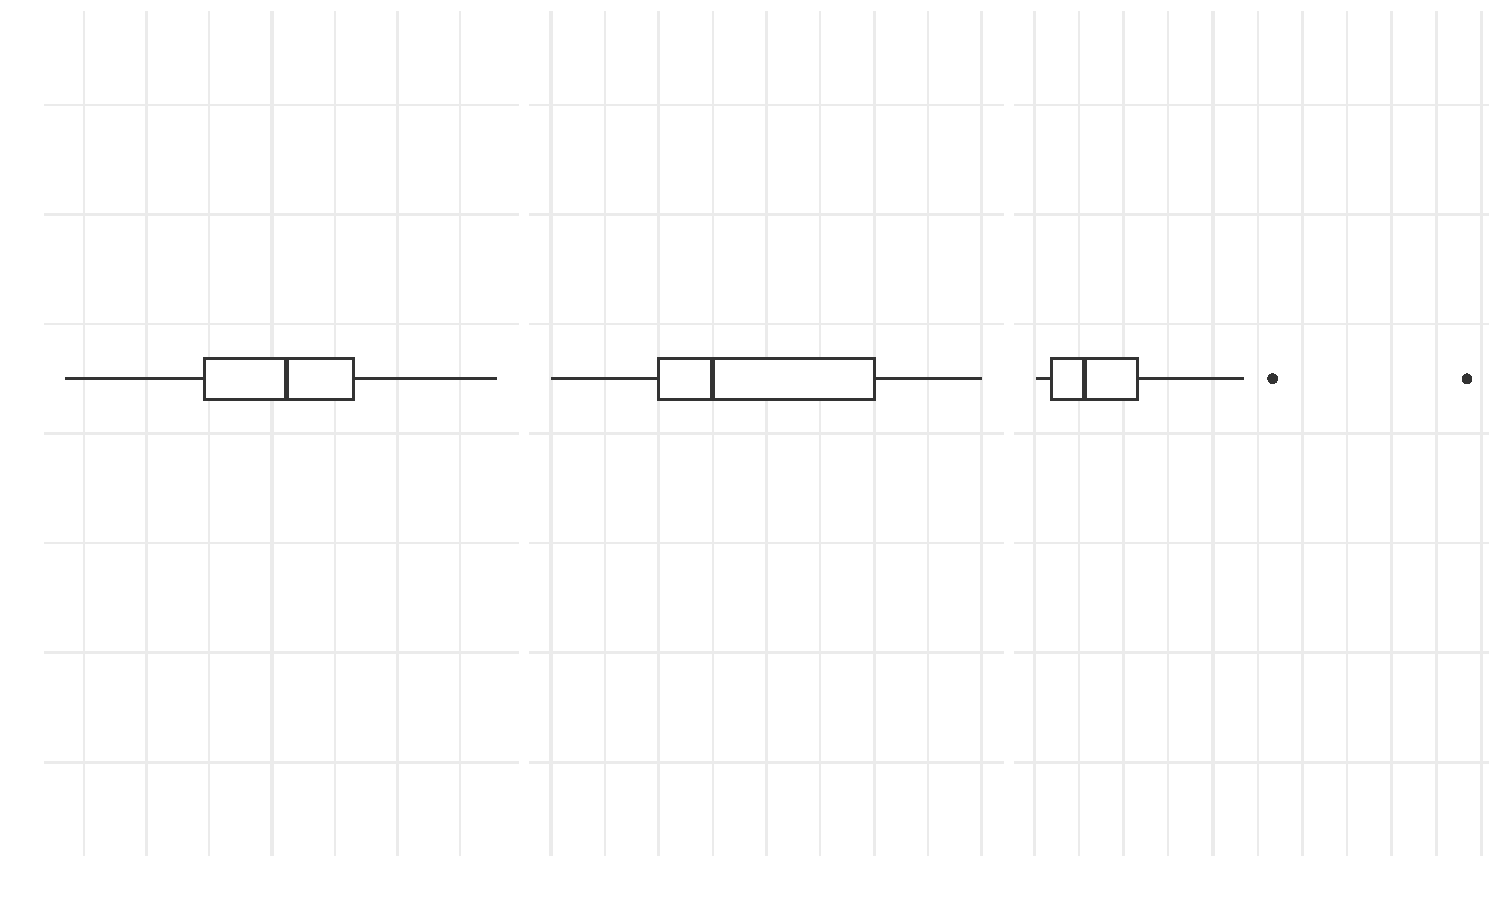
\includegraphics[width=\maxwidth]{img/desc-stat-11-1} 

}




 
\clearpage
% -----------------------------------------------------------------------

\section{Aufgabe \hfill (9 Punkte)}

\textit{Geben Sie grunds{\"a}tzlich Formeln und Rechenweg zur L{\"o}sung der
  Teilaufgaben mit an!} \\[1Ex]

%% --------------------------------------------------------------------
\hfill\href{https://youtu.be/ZrJhn2wPbq4}{
\includegraphics[width =
  2cm]{img/youtube}}\\[1Ex]
%% --------------------------------------------------------------------



\begin{enumerate}
\item Skizieren Sie $4$ Normalverteilungen \textit{in einer
    Abbildung} mit $\bar{y}_1 \neq \bar{y}_2 \neq \bar{y}_3 \neq \bar{y}_4$ und $s_1 \neq s_2 \neq s_3 \neq s_4$! \textbf{(3 Punkte)}
\item Beschriften Sie die Normalverteilungen mit den entsprechenden
  Parametern! \textbf{(2 Punkte)}
\item Erg{\"a}nzen Sie die Bereiche in der 68\% und 95\% der Beobachtungen
  fallen! Beschriften Sie die Grenzen der Bereiche mit der statistischen Ma{\ss}zahl! \textbf{(2 Punkte)}
\item Liegt Varianzhomogenit{\"a}t oder Varianzheterogenit{\"a}t vor? Begr{\"u}nden Sie
  Ihre Antwort! \textbf{(2 Punkte)}
\end{enumerate}

 
\clearpage
% -----------------------------------------------------------------------

\section{Aufgabe \hfill (9 Punkte)}

\textit{Geben Sie grunds{\"a}tzlich Formeln und Rechenweg zur L{\"o}sung der
  Teilaufgaben mit an!} \\[1Ex]

%% --------------------------------------------------------------------
\hfill\href{https://youtu.be/MiD42k4l5Ag}{
\includegraphics[width =
  2cm]{img/youtube}}\\[1Ex]
%% --------------------------------------------------------------------



\begin{enumerate}
\item Skizieren Sie in die unten stehenden, freien Abbildungen die
  Verteilungen, die sich nach der Abbildungs{\"u}berschrift ergeben! \textbf{(6
    Punkte)}
\item Beschriften Sie die Achsen der Abbildungen entsprechend! \textbf{(1
    Punkt)}
\item Achten Sie auf die entsprechende Skalierung der beiden Verteilungen
  in den Abbildungen! \textbf{(2 Punkte)}
\end{enumerate}



{\centering 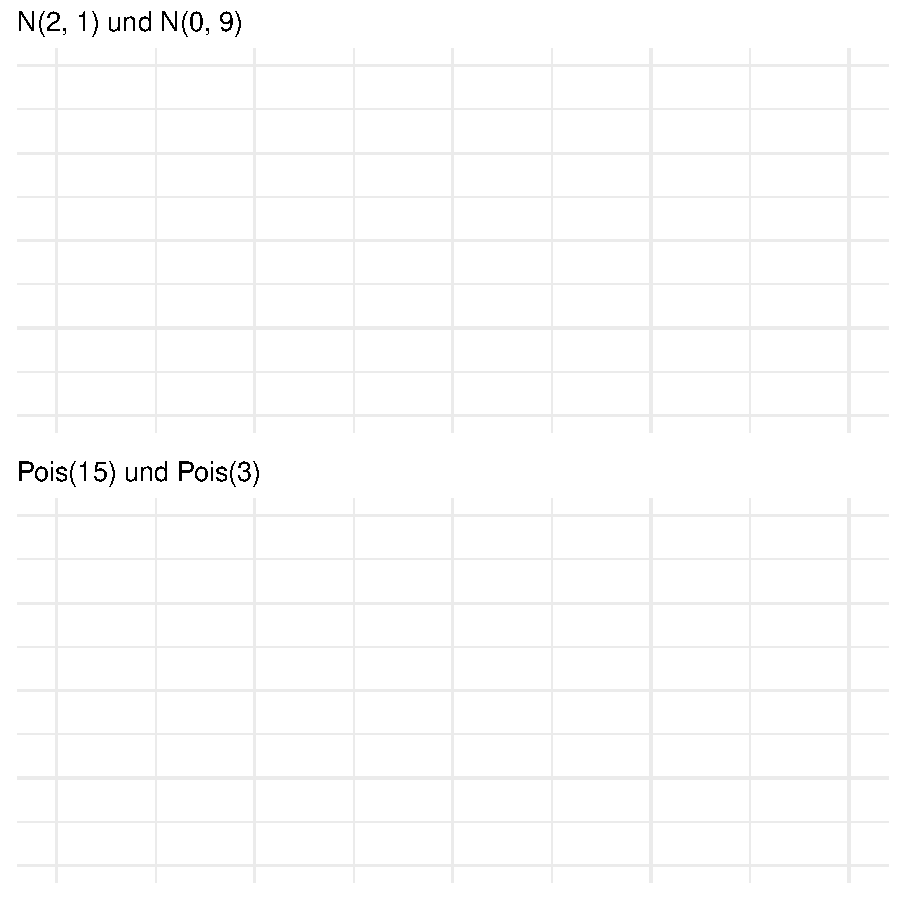
\includegraphics[width=\maxwidth]{img/histogram-01-1} 

}



 
\clearpage
% -----------------------------------------------------------------------

\section{Aufgabe \hfill (8 Punkte)}

\textit{Geben Sie grunds{\"a}tzlich Formeln und Rechenweg zur L{\"o}sung der
  Teilaufgaben mit an!} \\[1Ex]

%% --------------------------------------------------------------------
\hfill\href{https://youtu.be/oMdtYbDInYE}{
\includegraphics[width =
  2cm]{img/youtube}}\\[1Ex]
%% --------------------------------------------------------------------

Sie haben folgende Zahlenreihe $y$ vorliegen
$y = \{15, 17, 28, 18, 14, 14\}$.

\begin{enumerate}
\item Visualisieren Sie den Mittelwert von $y$ in der untenstehenden
  Abbildung! \textbf{(4 Punkte)}
\item Beschriften Sie die $Y$ und $X$-Achse entsprechend! \textbf{(2 Punkte)}
\item F{\"u}r die Berechnung der Varianz wird der Abstand der einzelnen Werte $y_i$
  zum Mittelwert $\bar{y}$ quadriert. Warum muss der Abstand, $y_i -
  \bar{y}$, in der Varianzformel quadriert werden?
  Erkl{\"a}ren Sie den Zusammenhang unter Ber{\"u}cksichtigung der Abbildung!
  \textbf{(2 Punkte)}  
\end{enumerate}



{\centering 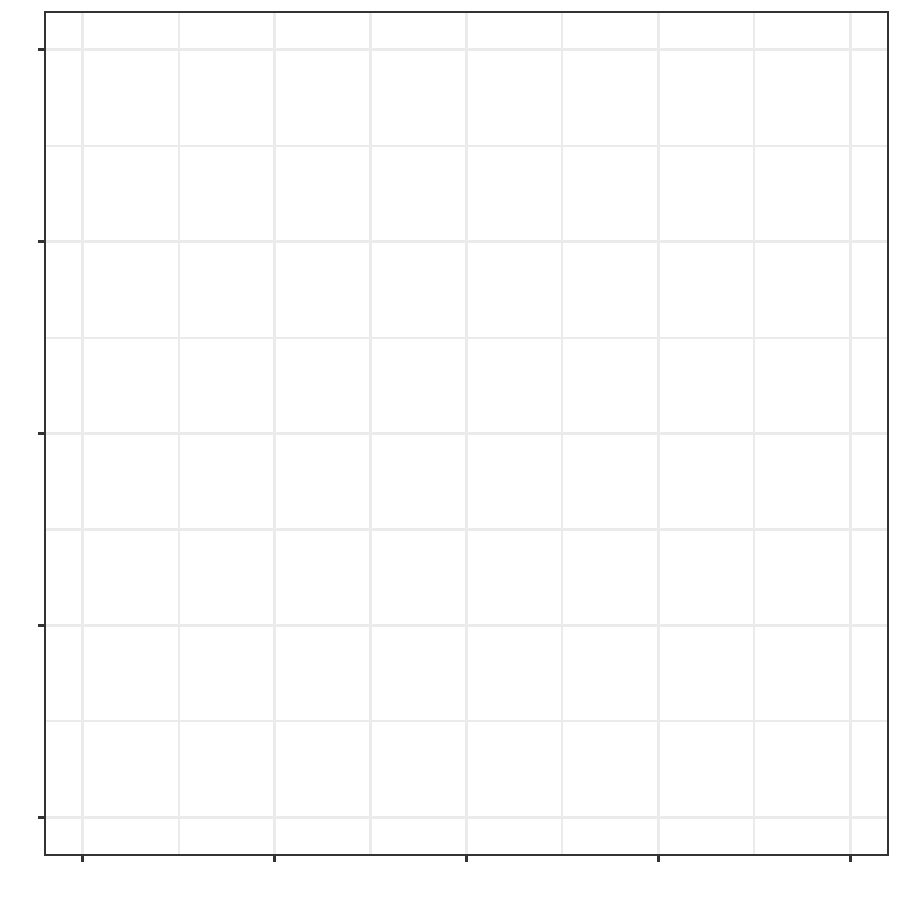
\includegraphics[width=\maxwidth]{img/desc-01-1} 

}


 
\clearpage
% -----------------------------------------------------------------------
\part{Statistisches Testen \& statistische Testtheorie}
% -----------------------------------------------------------------------  

\section{Aufgabe \hfill (9 Punkte)}

%% --------------------------------------------------------------------
\hfill\href{https://youtu.be/aHVYuFKTqZs}{
\includegraphics[width =
  2cm]{img/youtube}}\\[1Ex]
%% --------------------------------------------------------------------

Grundlage des statistischen Testen ist das Verst{\"a}ndnis von der
Grundgesamtheit (eng. \textit{population} oder \textit{ground truth}) und
der experimentellen Stichprobe (eng. \textit{sample}). 

\begin{enumerate}
\item Nennen Sie das statistische Verfahren und zwei konkrete Beispiele zur
  Durchf{\"u}hrung um von einer Grundgesamtheit auf eine Stichprobe zu
  gelangen! \textbf{(3 Punkte)}
\item Erkl{\"a}ren Sie den Zusammenhang zwischen Stichprobe und Grundgesamtheit
  an einem Schaubild! Beschriften Sie das Schaubild entsprechend!
  \textit{Nutzen Sie hierf{\"u}r als Veranschaulichung die K{\"o}rpergr{\"o}{\ss}e von
    M{\"a}nnern oder Frauen aus den Gummib{\"a}rchendaten!}  \textbf{(3 Punkte)}
\item Erweitern Sie das Schaubild um die Entstehung von $Pr(D|H_0)$!
  \textit{Nutzen Sie hierf{\"u}r als Veranschaulichung zus{\"a}tzlich die
    Gruppierungsvariable "`Modul"' aus den Gummib{\"a}rchendaten!}  \textbf{(3
    Punkte)}
\end{enumerate} 
\clearpage
% -----------------------------------------------------------------------

\section{Aufgabe \hfill (9 Punkte)}

%% --------------------------------------------------------------------
\hfill\href{https://youtu.be/Ric8ne39DtI}{
\includegraphics[width =
  2cm]{img/youtube}}\\[1Ex]
%% --------------------------------------------------------------------




F{\"u}r ein besseres Verst{\"a}ndnis der statistischen Testtheorie, auch
Null-Ritual genannt, kann eine Visualisierung als Kreuztabelle genutzt werden.  

\begin{enumerate}
\item Tragen Sie folgende statistische Fachbegriffe zur statistischen
  Testtheorie korrekt eine selbst erstellte Kreuztabelle ein! \textbf{(3
    Punkte)}
  \begin{center}
  \begin{tabular}{cccc}
  20\% & Testentscheidung & Richtige Entscheidung & (Unbekannte) Wahrheit \\
  \end{tabular}
  \end{center}
\item Erg{\"a}nzen Sie Ihre erstellte Kreuztabelle um vier weitere, passende
  Fachbegriffe zur statistischen Testtheorie! \textbf{(2 Punkte)}
\end{enumerate}

Die Entscheidungsfindung durch einen statistischen Test kann auch durch die
Analogie zu einem Feuermelder abgebildet werden. Dabei symbolisiert der
Feuermelder den statistischen Test und es soll getestet werden, ob ein Feuer
ausgebrochen ist.

\begin{enumerate}
  \setcounter{enumi}{2}    
\item In der Analogie des Feuermelders, wie lautet der $\alpha$-Fehler? \textbf{(1 Punkt)}
\item In der Analogie des Feuermelders, wie lautet der $\beta$-Fehler? \textbf{(1 Punkt)}
\item Wenn der Feuermelder einmal pro Tag messen w{\"u}rde, wie oft w{\"u}rde der
  Feuermelder mit einem $\alpha$ von 5\% in einem halben Jahr Alarm schlagen?
  Begr{\"u}nden Sie Ihre Antwort! \textbf{(2 Punkte)}
\end{enumerate}



 
\clearpage
% -----------------------------------------------------------------------

\section{Aufgabe \hfill (9 Punkte)}

\textit{Geben Sie grunds{\"a}tzlich Formeln und Rechenweg zur L{\"o}sung der
  Teilaufgaben mit an!} \\[1Ex]

%% --------------------------------------------------------------------
\hfill\href{https://youtu.be/32JjH1eyuTU}{
\includegraphics[width =
  2cm]{img/youtube}}\\[1Ex]
%% --------------------------------------------------------------------



Abgebildet ist die t-Verteilung unter der Anahme der G{\"u}ltigkeit der
Nullhypothese. \textit{Beachten Sie, dass im Folgenden keine
  numerisch korrekte Darstellung verlangt wird! Es gilt Erkennbarkeit vor
  Genauigkeit!}

\begin{enumerate}
\item Erg{\"a}nzen Sie eine beschriftete $x$-Achse! \textbf{(1 Punkt)}
\item Erg{\"a}nzen Sie "`$\bar{y}_1 = \bar{y}_2$"'! \textbf{(1 Punkt)} 
\item Erg{\"a}nzen Sie "`$95\%$"'! \textbf{(1 Punkt)}
\item Zeichnen Sie $T_{\alpha=5\%}$ in die Abbildung! \textbf{(1 Punkt)} 
\item Zeichnen Sie das Signifikanzniveau $\alpha$ in die Abbildung! Begr{\"u}nden
  Sie Ihre Antwort! \textbf{(2 Punkte)} 
\item Zeichnen Sie $-T_{D}$ in die Abbildung! \textbf{(1
    Punkt)}
\item Zeichnen Sie einen nicht signifikant p-Wert in die Abbildung! Begr{\"u}nden
  Sie Ihre Antwort! \textbf{(2 Punkte)}   
\end{enumerate}



{\centering 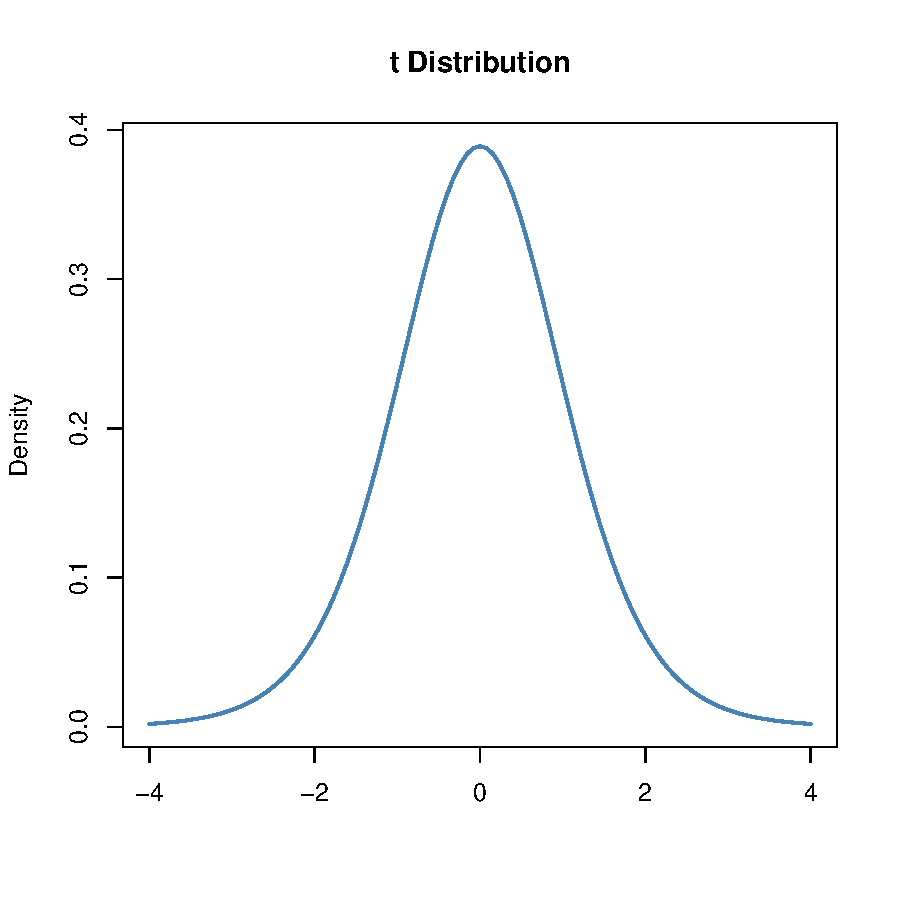
\includegraphics[width=\maxwidth]{img/statistisches-testen-3-1} 

}


 
\clearpage
% -----------------------------------------------------------------------

\section{Aufgabe \hfill (10 Punkte)}

%% --------------------------------------------------------------------
\hfill\href{https://youtu.be/CN_O4fYPbhs}{
\includegraphics[width =
  2cm]{img/youtube}}\\[1Ex]
%% --------------------------------------------------------------------



Sie rechnen einen t-Test f{\"u}r Gruppenvergleiche der Mittelwerte. Sie
sch{\"a}tzen den Unterschied zwischen dem mittleren Trockengewicht nach D{"u}ngergabe zu einer unbehandelten
Kontrolle.

\begin{enumerate}
\item Beschriften Sie die untenstehende Abbildung mit der
  Signifikanzschwelle! Begr{\"u}nden Sie Ihre Antwort! \textbf{(2 Punkte)}
\item Erg{\"a}nzen Sie eine \textit{in den Kontext passende} Relevanzschwelle!
  Begr{\"u}nden Sie Ihre Antwort! \textbf{(2 Punkte)} 
\item Skizieren Sie in die
  untenstehende Abbildung sechs einzelne Konfidenzintervalle (a-f) mit den
  jeweiligen Eigenschaften! \textbf{(6 Punkte)}
  \begin{itemize}
  \item[(a)] Ein signifikantes, relevantes 90\% Konfidenzintervall. 	
  \item[(b)] Ein 95\% Konfidenzintervall mit niedriger Fallzahl $n$ in der Stichprobe als der Rest 95\% der Konfidenzintervalle 	
  \item[(c)] Ein 95\% Konfidenzintervall mit h{"o}herer Fallzahl $n$ in der Stichprobe als der Rest der 95\% Konfidenzintervalle 	
  \item[(d)] Ein nicht signifikantes, nicht relevantes 95\% Konfidenzintervall 
  \item[(e)] Ein signifikantes, relevantes 95\% Konfidenzintervall
  \item[(f)] Ein signifikantes, nicht relevantes 95\% Konfidenzintervall
  \end{itemize}
\end{enumerate}

\begin{center}
  
\includegraphics[height = 12cm]{/Users/kruppajo/work/GitHub/exam/question/img/statistisches-testen-04}
\end{center}


 
\clearpage
% -----------------------------------------------------------------------

\section{Aufgabe \hfill (10 Punkte)}

\textit{Geben Sie grunds{\"a}tzlich Formeln und Rechenweg zur L{\"o}sung der
  Teilaufgaben mit an!} \\[1Ex]

%% --------------------------------------------------------------------
\hfill\href{https://youtu.be/FgZmpnEWDag}{
\includegraphics[width =
  2cm]{img/youtube}}\\[1Ex]
%% --------------------------------------------------------------------



Beim statistischen Testen gibt es einen Zusammenhang zwischen dem Effekt,
der Streuung sowie der Fallzahl. Gegeben sei die Formel f{\"u}r den Student
t-Test auf den die folgenden {\"U}berlegungen basieren sollen. Welche
Auswirkung hat die {\"A}nderungen der jeweiligen statistischen Ma{\ss}zahl des
Effekts $\Delta$, der Streuung $s$ und der Fallzahl $n$ auf die Teststistik
$T_{D}$, den p-Wert $Pr(D|H_0)$ sowie dem Konfidenzintervall
$KI_{1-\alpha}$?

\begin{enumerate}
\item Visualisieren Sie den Zusammenhang zwischen der Teststatiatik
  $T_{D}$ und dem p-Wert $Pr(D|H_0)$ f{\"u}r sich ver{\"a}ndernde $T_{D}$-Werte!
  \textit{Geben Sie daf{\"u}r ein numerisches Beispiel in dem Sie drei
    $T_{D}$-Werte und deren Einfluss auf den p-Wert vergleichen!}
  \textbf{(3 Punkte)}  
\item  F{\"u}llen Sie die untenstehende Tabelle aus in dem Sie die {\"A}nderung der
  statistischen Ma{\ss}zahlen auf die Teststatistik, den p-Wert sowie das
  Konfidenzintervall in \textit{einem} Wort oder Symbol beschreiben! \textbf{(4 Punkte)}
\begin{center}
  \large
  \begin{tabular}[c]{l|c|c|c|l|c|c|c}
    & $T_{D}$ & $Pr(D|H_0)$ & $KI_{1-\alpha}$ & & $T_{D}$ & $Pr(D|H_0)$ & $KI_{1-\alpha}$\strut\\ 
    \hline
    \textbf{$\Delta\; \uparrow$} & \hspace{1.8cm} & \hspace{1.8cm}  & \hspace{1.8cm} & \textbf{
                                                          $\Delta\; \downarrow$} &
                                                                          \hspace{1.8cm} & \hspace{1.8cm}  & \hspace{1.8cm}\strut\\
    \hline
        \textbf{$s\; \uparrow$} & \hspace{1.8cm} & \hspace{1.8cm}  & \hspace{1.8cm} & \textbf{
                                                          $s\; \downarrow$} &
                                                                          \hspace{1.8cm}
                                                & \hspace{1.8cm}  & \hspace{1.8cm}\strut\\
    \hline
        \textbf{$n\; \uparrow$} & \hspace{1.8cm} & \hspace{1.8cm}  & \hspace{1.8cm} & \textbf{
                                                          $n\; \downarrow$} &
                                                                          \hspace{1.8cm}
                                                & \hspace{1.8cm}  & \hspace{1.8cm}\strut\\
    \hline
  \end{tabular}
\end{center}
\item Visualisieren Sie ein 95\%-iges Konfidenzintervall im Vergleich
  zu einem 90\%-igen Konfidenzintervall! Begr{\"u}nden Sie Ihre Visualisierung anhand der Formel
  des Konfidenzintervalls des t-Tests mathematisch! \textbf{(3 Punkte)} 
\end{enumerate} 
\clearpage
% -----------------------------------------------------------------------
\part{Der Student t-Test, Welch t-Test \& gepaarter t-Test}
% -----------------------------------------------------------------------

\section{Aufgabe \hfill (9 Punkte)}

\textit{Geben Sie grundsätzlich Formeln und Rechenweg zur Lösung der Teilaufgaben mit an!} \\[1Ex]
 

 
%% --------------------------------------------------------------------
\begin{minipage}[t]{0.5\textwidth}

\includegraphics[width = 1.3cm]{/Users/kruppajo/work/GitHub/exam/avatare/Jessica.png}
\end{minipage}
\begin{minipage}[t]{0.5\textwidth}
\hfill
\href{https://youtu.be/eejS2uG4o-M}{
\includegraphics[width = 2cm]{img/youtube}}\\[1Ex]
\end{minipage}
\vspace{1ex}
%% --------------------------------------------------------------------



Jessica ist im Teuteburgerwald für einen Pilotexperiment mit sehr geringer Fallzahl $(n_1 = n_2 = 3)$ mit Kartoffeln. Allein diese Tatsache ist für sie eine Erzählung wert. Für ihrer Hausarbeit musste sie einen Versuch in einer Klimakammer mit Kartoffeln durchführen und das sollte laut ihrem Betreuer an diesem Ort besonders gut gelingen, da man hier gut neue technische Anlagen und Behandlungen fernab der Bevölkerung testen könne. Zeugen gibt es hier jedenfalls keine. Gar keine. Alleine sein hilft jetzt aber nur bedingt, denn ihre Behandlung Lüftungssystemen und Folientunneln ($ctrl$ und $tornado$) und der Messwert Frischegewicht [kg/ha] sollen mit einem t-Test ausgewertet werden. Immerhin weiß sie, dass ihr Messwert einer Normalverteilung folgt. 

\begin{table}[!h]
\centering
\begin{tabular}{cc}
\toprule
treatment & weight\\
\midrule
ctrl & 15.9\\
dose & 21.9\\
dose & 16.3\\
dose & 18.0\\
ctrl & 10.9\\
\addlinespace
ctrl & 6.4\\
\bottomrule
\end{tabular}
\end{table}



Leider kennt sich Jessica mit der Berechnung eines t-Tests überhaupt nicht aus. Deshalb braucht sie bei der Berechnung Ihre Hilfe!

\begin{enumerate}
  \item Formulieren Sie die wissenschaftliche Fragestellung! \textbf{(1 Punkt)}
  \item Bestimmen Sie die Teststatistik $T_{D}$ eines Student t-Tests! \textbf{(3 Punkte)}
  \item Treffen Sie mit $T_{\alpha = 5\%} = 1.64$ eine Aussage zur Nullhypothese! Begründen Sie Ihre Antwort! \textbf{(2 Punkte)}
  \item Berechnen Sie den Effekt des Student t-Tests! \textbf{(1 Punkt)}
  \item Formulieren Sie eine Antwort an Jessica über das Ergebnis Ihrer statistischen Analyse! \textbf{(2 Punkte)}
\end{enumerate} 
\clearpage
% -----------------------------------------------------------------------

\section{Aufgabe \hfill (12 Punkte)}

\textit{Geben Sie grundsätzlich Formeln und Rechenweg zur Lösung der Teilaufgaben mit an!} \\[1Ex]
 

 
%% --------------------------------------------------------------------
\begin{minipage}[t]{0.5\textwidth}

\includegraphics[width = 1.3cm]{/Users/kruppajo/work/GitHub/exam/avatare/Tina.png}
\end{minipage}
\begin{minipage}[t]{0.5\textwidth}
\hfill
\href{https://youtu.be/Cq_rF_z4xOk}{\includegraphics[width = 2cm]{img/youtube}}\\[1Ex]
\end{minipage}
\vspace{1ex}
%% --------------------------------------------------------------------



Der t-Test. Tina erschaudert. Ein mächtiges Werkzeug in den Händen desjenigen, der einen normalverteilten Messwert ($Y$) hat. Aber erstmal überhaupt den t-Test rechnen können. Wie sah das Experiment von Tina überhaupt aus? Tina hat ein Gewächshausexperiment mit Kartoffeln durchgeführt. Dabei wurde die Behandlung Düngestufen ($ctrl$ und $high$) an den Kartoffeln getestet. Gemessen hat Tina dann als Messwert Trockengewicht [kg/ha]. Warum der Versuch im Emsland für ihre Abschlussarbeit stattfinden musste, ist ihr bis heute ein Rätsel. Egal. Gibt es jetzt einen Zusammenhang zwischen der Behandlung und Trockengewicht [kg/ha]?

\begin{table}[!h]
\centering
\begin{tabular}{cc}
\toprule
Düngestufen & Trockengewicht\\
\midrule
high & 48.3\\
high & 51.0\\
ctrl & 28.5\\
high & 42.0\\
high & 32.5\\
\addlinespace
ctrl & 42.2\\
high & 40.4\\
ctrl & 33.8\\
ctrl & 41.5\\
high & 42.9\\
\addlinespace
ctrl & 38.7\\
ctrl & 41.0\\
ctrl & 36.7\\
high & 35.5\\
ctrl & 34.0\\
\addlinespace
ctrl & 40.2\\
high & 54.3\\
high & 34.7\\
\bottomrule
\end{tabular}
\end{table}



Leider kennt sich Tina mit der Berechnung eines t-Tests überhaupt nicht aus. Deshalb braucht sie bei der Berechnung Ihre Hilfe!

\begin{enumerate}
  \item Formulieren Sie die wissenschaftliche Fragestellung! \textbf{(1 Punkt)}
  \item Formulieren Sie das statistische Hypothesenpaar! \textbf{(1 Punkt)}
  \item Bestimmen Sie die Teststatistik $T_{D}$ eines Student t-Tests! \textbf{(3 Punkte)}
\item Treffen Sie mit $T_{\alpha = 5\%} = 1.84$ eine Aussage zur Nullhypothese! Begründen Sie Ihre Antwort! \textbf{(2 Punkte)}
\item Berechnen Sie den Effekt des Student t-Tests! \textbf{(1 Punkt)}
\item Wenn Sie \textit{einen} Unterschied zwischen den Behandlungsgruppen erwarten würden, wie groß wäre dann die Teststatistik $T_{D}$? Begründen Sie Ihre Antwort! \textbf{(2 Punkte)}
\item Formulieren Sie eine Antwort an Tina über das Ergebnis Ihrer statistischen Analyse! \textbf{(2 Punkte)}
\end{enumerate} 
\clearpage
% -----------------------------------------------------------------------

\section{Aufgabe \hfill (12 Punkte)}

\textit{Geben Sie grundsätzlich Formeln und Rechenweg zur Lösung der Teilaufgaben mit an!} \\[1Ex]
 

 
%% --------------------------------------------------------------------
\begin{minipage}[t]{0.5\textwidth}
\includegraphics[width = 1.3cm]{/Users/kruppajo/work/GitHub/exam/avatare/Paula.png}
\end{minipage}
\begin{minipage}[t]{0.5\textwidth}
\hfill
\href{https://youtu.be/TbSEOMCQYl4}{\includegraphics[width = 2cm]{img/youtube}}\\[1Ex]
\end{minipage}
\vspace{1ex}
%% --------------------------------------------------------------------



Paula ist in der Uckermark für einen Versuch mit Kartoffeln. Allein diese Tatsache ist für sie eine Erzählung wert. Für ihre Abschlussarbeit musste sie einen Versuch in einer Klimakammer mit Kartoffeln durchführen und das sollte laut ihrem Betreuer an diesem Nichtort besonders gut gelingen. Ablenkung gibt es jedenfalls keine. Gar keine. Alleine sein hilft jetzt aber nur bedingt, denn ihre Behandlung Genotypen ($AA$ und $BB$) und der Messwert Frischegewicht [kg/ha] sollen mit einem t-Test ausgewertet werden. Immerhin weiß sie, dass ihr Messwert einer Normalverteilung folgt. 

\begin{table}[!h]
\centering
\begin{tabular}{cc}
\toprule
Genotypen & Frischegewicht\\
\midrule
AA & 47.4\\
AA & 44.2\\
BB & 49.9\\
BB & 44.2\\
AA & 43.3\\
\addlinespace
BB & 44.7\\
BB & 42.3\\
AA & 44.9\\
BB & 45.4\\
BB & 46.8\\
\addlinespace
AA & 54.9\\
BB & 47.5\\
AA & 44.0\\
AA & 38.6\\
AA & 51.0\\
\addlinespace
AA & 42.7\\
AA & 45.4\\
BB & 38.3\\
BB & 42.2\\
AA & 42.4\\
\bottomrule
\end{tabular}
\end{table}



Leider kennt sich Paula mit der Berechnung eines t-Tests überhaupt nicht aus. Deshalb braucht sie bei der Berechnung Ihre Hilfe!

\begin{enumerate}
  \item Formulieren Sie die wissenschaftliche Fragestellung! \textbf{(1 Punkt)}
  \item Formulieren Sie das statistische Hypothesenpaar! \textbf{(1 Punkt)}
  \item Bestimmen Sie die Teststatistik $T_{D}$ eines  Welch t-Tests! \textbf{(3 Punkte)}
  \item Treffen Sie mit $T_{\alpha = 5\%} = 1.84$ eine Aussage zur Nullhypothese! Begründen Sie Ihre Antwort! \textbf{(2 Punkte)}
\item Berechnen Sie das 95\% Konfidenzintervall. Welche Annahmen haben Sie getroffen? \textbf{(2 Punkte)}
\item Nennen Sie den statistischen Grund, warum Sie sich zwischen einem Student t-Test und einem Welch t-Test entscheiden müssen! \textbf{(1 Punkt)}
\item Formulieren Sie eine Antwort an Paula über das Ergebnis Ihrer statistischen Analyse! \textbf{(2 Punkte)}
\end{enumerate} 
\clearpage
% -----------------------------------------------------------------------

\section{Aufgabe \hfill (11 Punkte)}

\textit{Geben Sie grundsätzlich Formeln und Rechenweg zur Lösung der Teilaufgaben mit an!} \\[1Ex]
 

 
%% --------------------------------------------------------------------
\begin{minipage}[t]{0.5\textwidth}
\includegraphics[width = 1.3cm]{/Users/kruppajo/work/GitHub/exam/avatare/Steffen.png}\hspace{-4mm}\includegraphics[width = 1.3cm]{/Users/kruppajo/work/GitHub/exam/avatare/Yuki.png}
\end{minipage}
\begin{minipage}[t]{0.5\textwidth}
\hfill
\href{https://youtu.be/QR90zyn0Iz8}{\includegraphics[width = 2cm]{img/youtube}}
\end{minipage}
\vspace{1ex}
%% --------------------------------------------------------------------



Es gibt ja immer die Möglichkeit sich Hilfe zu holen. Das geht natürlich auch immer in einem Projektbericht. Deshalb arbeiten Yuki und Steffen gemeinsam an einem Projektbericht. Das macht dann auch die Analyse ihres Hauptversuches einfacher. Zwar hat jeder von ihnen noch ein Subthema, aber auch da kann man sich ja helfen. In dem Hauptversuch wurde Folgendes von den beiden gemacht. Yuki und Steffen haben sich Kartoffeln angeschaut. Dabei geht um Zusammenhang zwischen Ausgeizen ($ctrl$ und $28d$) und Frischegewicht [kg/ha]. Jetzt sollen beide einen gepaarten t-Test rechnen.

\begin{table}[!h]
\centering
\begin{tabular}{ccc}
\toprule
ID & treatment & freshmatter\\
\midrule
10 & 28d & 55.5\\
10 & ctrl & 25.3\\
9 & ctrl & 22.4\\
8 & 28d & 48.4\\
2 & 28d & 45.0\\
\addlinespace
9 & 28d & 34.0\\
5 & ctrl & 24.2\\
7 & 28d & 53.6\\
6 & ctrl & 33.7\\
6 & 28d & 47.0\\
\addlinespace
2 & ctrl & 31.6\\
7 & ctrl & 28.5\\
3 & 28d & 45.8\\
5 & 28d & 45.6\\
1 & 28d & 46.4\\
\addlinespace
8 & ctrl & 28.4\\
4 & 28d & 46.3\\
3 & ctrl & 33.4\\
4 & ctrl & 20.9\\
1 & ctrl & 29.4\\
\bottomrule
\end{tabular}
\end{table}



Leider kennen sich Yuki und Steffen mit der Berechnung eines gepaarten t-Tests überhaupt nicht aus. Deshalb brauchen sie beide bei der Berechnung Ihre Hilfe!

\begin{enumerate}
  \item Formulieren Sie die wissenschaftliche Fragestellung! \textbf{(1 Punkt)}
  \item Formulieren Sie das statistische Hypothesenpaar! \textbf{(1 Punkt)}
  \item Bestimmen Sie die Teststatistik $T_{D}$ eines gepaarten t-Tests! \textbf{(3 Punkte)}
  \item Treffen Sie mit $T_{\alpha = 5\%} = 2.04$ eine Aussage zur Nullhypothese! Begründen Sie Ihre Antwort! \textbf{(2 Punkte)}
\item Schätzen Sie den $p$-Wert des gepaarten t-Tests ab! Begründen Sie Ihre Antwort mit einer Skizze! \textbf{(2 Punkte)}
\item Formulieren Sie eine Antwort an Yuki über das Ergebnis Ihrer statistischen Analyse! \textbf{(2 Punkte)}
\end{enumerate}


 
\clearpage
% -----------------------------------------------------------------------

\section{Aufgabe \hfill (10 Punkte)}

\textit{Geben Sie grundsätzlich Formeln und Rechenweg zur Lösung der Teilaufgaben mit an!} \\[1Ex]
 

 
%% --------------------------------------------------------------------
\begin{minipage}[t]{0.5\textwidth}
\includegraphics[width = 1.3cm]{/Users/kruppajo/work/GitHub/exam/avatare/Jessica.png}\hspace{-4mm}\includegraphics[width = 1.3cm]{/Users/kruppajo/work/GitHub/exam/avatare/Jonas.png}\hspace{-4mm}\includegraphics[width = 1.3cm]{/Users/kruppajo/work/GitHub/exam/avatare/Paula.png}
\end{minipage}
\begin{minipage}[t]{0.5\textwidth}
\hfill
\href{https://youtu.be/exDo7AyHl4Q}{\includegraphics[width = 2cm]{img/youtube}}
\end{minipage}
\vspace{1ex}
%% --------------------------------------------------------------------



Jessica und Jonas sind bei Paula um sich Hilfe in \Rlogo zu holen. Die beiden hatten zwar schon erste Kontakte mit \Rlogo sind sich aber unsicher bei der Interpetierung der Ausgabe eines t-Tests für ihren gemeinsamen Versuch. In einem Projektbericht haben sie zusammen Kartoffeln untersucht. Dabei ging es um den Zusammenhang zwischen der Behandlung Lüftungssystemen und Folientunneln ($ctrl$ und $tornado$) und dem Messwert Trockengewicht [kg/ha]. Der Versuch wurde in einem Versuch in einer Klimakammer im Emsland durchgeführt. Nach des Betreuers ist der Messwert Trockengewicht [kg/ha] normalverteilt und ein t-Test passt daher. Das wird jetzt nicht mehr angezweifel...

\begin{knitrout}
\definecolor{shadecolor}{rgb}{0.969, 0.969, 0.969}\color{fgcolor}\begin{kframe}
\begin{verbatim}
## 
## 	Two Sample t-test
## 
## data:  Trockengewicht by Lüftungssystemen
## t = -3.4749, df = 17, p-value = 0.002898
## alternative hypothesis: true  is not equal to [condensed]
## 95 percent confidence interval:
##  -16.905600  -4.132178
## sample estimates:
##    mean in group ctrl mean in group tornado 
##              25.87000              36.38889
\end{verbatim}
\end{kframe}
\end{knitrout}

Helfen Sie Paula bei der Interpretation des t-Tests! Sonst geht es auch für Jessica und Jonas nicht weiter.
  
\begin{enumerate}
  \item Formulieren Sie die wissenschaftliche Fragestellung! \textbf{(1 Punkt)}
  \item Formulieren Sie das statistische Hypothesenpaar! \textbf{(1 Punkt)}
\item Liegt ein signifikanter Unterschied zwischen den Gruppen vor? Begründen Sie Ihre Antwort! \textbf{(2 Punkte)}
\item Skizzieren Sie eine Abbildung in der Sie $T_{D}$, $Pr(D|H_0)$, $A=0.95$, sowie $T_{\alpha=5\%} = |2.11|$ einzeichnen! \textbf{(4 Punkte)}
\item Beschriften Sie die Abbildung! \textbf{(1 Punkt)}  
\item Berechnen Sie den Effekt des t-Tests! \textbf{(1 Punkt)}
\end{enumerate} 
\clearpage
% -----------------------------------------------------------------------

\section{Aufgabe \hfill (8 Punkte)}

\textit{Geben Sie grundsätzlich Formeln und Rechenweg zur Lösung der Teilaufgaben mit an!} \\[1Ex]
 

 
%% --------------------------------------------------------------------
\begin{minipage}[t]{0.5\textwidth}
\includegraphics[width = 1.3cm]{/Users/kruppajo/work/GitHub/exam/avatare/Alex.png}\hspace{-4mm}\includegraphics[width = 1.3cm]{/Users/kruppajo/work/GitHub/exam/avatare/Jessica.png}\hspace{-4mm}\includegraphics[width = 1.3cm]{/Users/kruppajo/work/GitHub/exam/avatare/Steffen.png}
\end{minipage}
\begin{minipage}[t]{0.5\textwidth}
\hfill
\href{https://youtu.be/wJqsNV1hOW8}{\includegraphics[width = 2cm]{img/youtube}}
\end{minipage}
\vspace{1ex}
%% --------------------------------------------------------------------



\Rlogo ist schon ein tolles Programm, wenn man mit dem Ding umgehen kann. Super umgehen kann damit Alex. Deshalb sind auch Steffen und Jessica bei ihm um sich bei einem gemeinsamen Projekt helfen zu lassen. Beide arbeiten gemeinsam an einer Abschlussarbeit. In dem zu beschreibenden Versuch geht es im Emsland um einem Feldexperiment mit Kartoffeln. Dabei ging darum herauszufinden, ob es einen Zusammenhang zwischen der Behandlung Lüftungssystemen und Folientunneln ($ctrl$ und $tornado$) und dem Messwert Trockengewicht [kg/ha] gibt. Da der Messwert Trockengewicht [kg/ha] normalverteilt ist kann ein t-Test gerechnet werden.

\begin{knitrout}
\definecolor{shadecolor}{rgb}{0.969, 0.969, 0.969}\color{fgcolor}\begin{kframe}
\begin{verbatim}
## 
## 	Two Sample t-test
## 
## data:  Trockengewicht by Lüftungssystemen
## t = 1.9217, df = 16, p-value = 0.07264
## alternative hypothesis: true  is not equal to [condensed]
## 95 percent confidence interval:
##  -0.7128455 14.5362221
## sample estimates:
##    mean in group ctrl mean in group tornado 
##              47.95714              41.04545
\end{verbatim}
\end{kframe}
\end{knitrout}

Helfen Sie Alex bei der Interpretation des t-Tests! Sonst geht es auch für Steffen und Jessica nicht weiter.

\begin{enumerate}
  \item Formulieren Sie die wissenschaftliche Fragestellung! \textbf{(1 Punkt)}
  \item Formulieren Sie das statistische Hypothesenpaar! \textbf{(1 Punkt)}
\item Liegt ein signifikanter Unterschied zwischen den Gruppen vor? Begründen Sie Ihre Antwort! \textbf{(2 Punkte)}
\item Skizieren Sie das sich ergebende 95\% Konifidenzintervall! \textbf{(2 Punkte)}
\item Beschriften Sie die Abbildung und das 95\% Konfidenzintervall entsprechend! \textbf{(2 Punkte)}  
\end{enumerate} 
\clearpage
% -----------------------------------------------------------------------

\section{Aufgabe \hfill (9 Punkte)}

\textit{Geben Sie grundsätzlich Formeln und Rechenweg zur Lösung der Teilaufgaben mit an!} \\[1Ex]
 

 
%% --------------------------------------------------------------------
\begin{minipage}[t]{0.5\textwidth}
\includegraphics[width = 1.3cm]{/Users/kruppajo/work/GitHub/exam/avatare/Jessica.png}\hspace{-4mm}\includegraphics[width = 1.3cm]{/Users/kruppajo/work/GitHub/exam/avatare/Paula.png}\hspace{-4mm}NA
\end{minipage}
\begin{minipage}[t]{0.5\textwidth}
\hfill
\href{https://youtu.be/w62HJlbN28U}{\includegraphics[width = 2cm]{img/youtube}}
\end{minipage}
\vspace{1ex}
%% --------------------------------------------------------------------



'Mit dem R Paket \texttt{\{emmeans\}} können wir gleich die Gruppenvergleiche rechnen und uns das \textit{compact letter displac}' ausgeben lassen!', verkündet Jessica sichtlich stolz. 'Nach Meinung des Betreuers soll es aber nur erstmal ein t-Test sein. Und die Ausgabe ist schon wirr genug.', merkt Paula an. Paula und Paula sind bei Jessica um sich in \Rlogo helfen zu lassen. Die beiden waren 2 Monate im Wendland um einen Versuch mit Kartoffeln in einem Freilandversuch durchzuführen. Ziel war es das Outcome ($Y$) Proteingehalt [g/kg] zu bestimmen.

\begin{knitrout}
\definecolor{shadecolor}{rgb}{0.969, 0.969, 0.969}\color{fgcolor}\begin{kframe}
\begin{verbatim}
## 
## 	Two Sample t-test
## 
## data:  Proteingehalt by Lichtstufen
## t = 3.1677, df = 15, p-value = 0.006371
## alternative hypothesis: true  is not equal to [condensed]
## 95 percent confidence interval:
##   3.67302 18.78254
## sample estimates:
##  mean in group none mean in group 600lm 
##            35.35000            24.12222
\end{verbatim}
\end{kframe}
\end{knitrout}

Helfen Sie Jessica bei der Interpretation des t-Tests! Sonst geht es auch für Paula und Paula nicht weiter.
  
\begin{enumerate}
  \item Formulieren Sie die wissenschaftliche Fragestellung! \textbf{(1 Punkt)}
  \item Formulieren Sie das statistische Hypothesenpaar! \textbf{(1 Punkt)}
\item Liegt ein signifikanter Unterschied zwischen den Gruppen vor?
  Begründen Sie Ihre Antwort! \textbf{(2 Punkte)}
\item Skizieren Sie die sich ergebenden Boxplot!
  Welche Annahmen an die Daten haben Sie getroffen? Begründen Sie Ihre
  Antwort! \textbf{(2 Punkte)} 
\item Skizieren Sie die sich ergebenden Barplots! \textbf{(2 Punkte)}
\item Berechnen Sie den Effekt des t-Tests! \textbf{(1 Punkt)}
\end{enumerate}
 
\clearpage
% -----------------------------------------------------------------------

\section{Aufgabe \hfill (8 Punkte)}

\textit{Geben Sie grundsätzlich Formeln und Rechenweg zur Lösung der Teilaufgaben mit an!} \\[1Ex]
 

 
%% --------------------------------------------------------------------
\begin{minipage}[t]{0.5\textwidth}
\includegraphics[width = 1.3cm]{/Users/kruppajo/work/GitHub/exam/avatare/Mark.png}\hspace{-4mm}\includegraphics[width = 1.3cm]{/Users/kruppajo/work/GitHub/exam/avatare/Nilufar.png}
\end{minipage}
\begin{minipage}[t]{0.5\textwidth}
\hfill
\href{https://youtu.be/kHmfEmU6lrk}{\includegraphics[width = 2cm]{img/youtube}}
\end{minipage}
\vspace{1ex}
%% --------------------------------------------------------------------



Nilufar und Mark haben sich dazu entschieden zusammenzuarbeiten. Das sollte alles etwas einfacher machen. Jeder hat zwar ein getrenntes Themenfeld aber den Hauptversuch machen beide gemeinsam. Das hat sich schonmal als gut Idee soweit herausgestellt. In einer Hausarbeit sollen beide herausfinden, ob es einen Zusammenhang zwischen Ausgeizen ($ctrl$ und $28d$) und Trockengewicht [kg/ha] gibt. Die Besonderheit ist hierbei, dass die Messungen an der gleichen Beobachtung stattfinden. Beide messen also zweimal an den gleichen Kartoffeln. Hier muss dann wohl auf einen normalverteilten Messwert ($Y$) ein gepaarter t-Test gerechnet werden. Leider kennen sich beide nicht sehr gut in \Rlogo aus.

\begin{knitrout}
\definecolor{shadecolor}{rgb}{0.969, 0.969, 0.969}\color{fgcolor}\begin{kframe}
\begin{verbatim}
## 
## 	Paired t-test
## 
## data:  Trockengewicht by Ausgeizen
## t = -1.4326, df = 8, p-value = 0.1899
## alternative hypothesis: true  is not equal to [condensed]
## 95 percent confidence interval:
##  -11.714516   2.736738
## sample estimates:
## mean difference 
##       -4.488889
\end{verbatim}
\end{kframe}
\end{knitrout}

Jetzt brauchen Nilufar und Mark Ihre Hilfe bei der Berechnung eines gepaarten t-Tests in \Rlogo um ihre Arbeit dann in diesem Semester noch abschließen zu können.

\begin{enumerate}
  \item Formulieren Sie die wissenschaftliche Fragestellung! \textbf{(1 Punkt)}
  \item Formulieren Sie das statistische Hypothesenpaar! \textbf{(1 Punkt)}
\item Liegt ein signifikanter Unterschied zwischen den Gruppen vor?
  Begründen Sie Ihre Antwort! \textbf{(2 Punkte)}
\item Skizzieren Sie das sich ergebende 95\% Konifidenzintervall! \textbf{(2 Punkte)}
\item Skizzieren Sie den sich ergebenden Boxplot der Differenzen! Welche Annahmen an die Daten haben Sie getroffen? Begründen Sie Ihre Antwort! \textbf{(2 Punkte)} 
\end{enumerate}
 
\clearpage
% -----------------------------------------------------------------------
\part{Die einfaktorielle \& zweifaktorielle ANOVA}
% -----------------------------------------------------------------------

\section{Aufgabe \hfill (11 Punkte)}

\textit{Geben Sie grundsätzlich Formeln und Rechenweg zur Lösung der Teilaufgaben mit an!} \\[1Ex]
 

 
%% --------------------------------------------------------------------
\begin{minipage}[t]{0.5\textwidth}
\includegraphics[width = 1.3cm]{/Users/kruppajo/work/GitHub/exam/avatare/Paula.png}\hspace{-4mm}\includegraphics[width = 1.3cm]{/Users/kruppajo/work/GitHub/exam/avatare/Tina.png}
\end{minipage}
\begin{minipage}[t]{0.5\textwidth}
\hfill
\href{https://youtu.be/kHmfEmU6lrk}{\includegraphics[width = 2cm]{img/youtube}}
\end{minipage}
\vspace{1ex}
%% --------------------------------------------------------------------



'Uff... die einfaktorielle ANOVA. Und wir können jetzt anhand der Visualisuierung sehen, ob da schon was signifikant ist?', Tina hebt die Augenbraue. 'Ja, können wir. Dafür müssen wir aber erstmal in \texttt{\{ggplot\}} uns die Daten anschauen. Oder wir zeichnen es flott mit der Hand. Geht auch.', meint Paula dazu. Tina hatte sich in einen Versuch in einer Klimakammer verschiedene Kartoffeln angeschaut. Dabei ging es herauszufinden, ob es einen Zusammenhang zwischen der Behandlung Lüftungssystemen und Folientunneln ($ctrl$, $storm$ und $tornado$) und dem Messwert Frischegewicht [kg/ha] gibt.

\begin{knitrout}
\definecolor{shadecolor}{rgb}{0.969, 0.969, 0.969}\color{fgcolor}\begin{table}[!h]
\centering
\begin{tabular}{cc}
\toprule
Lüftungssystemen & Frischegewicht\\
\midrule
storm & 38\\
storm & 41\\
tornado & 47\\
storm & 40\\
ctrl & 30\\
\addlinespace
ctrl & 30\\
tornado & 46\\
tornado & 47\\
ctrl & 30\\
tornado & 45\\
\addlinespace
tornado & 46\\
tornado & 43\\
ctrl & 30\\
ctrl & 31\\
ctrl & 29\\
\addlinespace
storm & 42\\
tornado & 49\\
ctrl & 29\\
storm & 41\\
\bottomrule
\end{tabular}
\end{table}

\end{knitrout}

Leider kennen sich Tina und Paula mit Darstellung einer einfaktoriellen ANOVA überhaupt nicht aus. Deshalb brauchen beide bei der Erstellung Ihre Hilfe! 

\begin{enumerate}
\item Erstellen  Sie  eine  Visualisierung  der  Datentabelle! Beschriften  Sie  die  Abbildung! \textbf{(2 Punkte)}
\item Benennen Sie die Visualisierung mit dem korrekten, statistischen Fachbegriff! \textbf{(1 Punkt)}
\item Zeichnen Sie folgende statistischen Maßzahlen passend ein! 
  \begin{itemize}
  \item Globale Mittelwert: $\beta_0$ \textbf{(1 Punkt)}
  \item Mittelwerte der einzelnen Behandlungsstufen: $\bar{y}_{0.5}$, $\bar{y}_{1.5}$ und $\bar{y}_{2.5}$ \textbf{(1 Punkt)}
  \item Mittelwertsdifferenz der einzelnen Behandlungsstufen: $\beta_{0.5}$, $\beta_{1.5}$ und $\beta_{2.5}$ \textbf{(1 Punkt)}
  \item Residuen oder Fehler: $\epsilon$ \textbf{(1 Punkt)}
  \end{itemize}
\item Liegt ein \textit{vermutlicher} signifikanter Unterschied vor? Begründen Sie Ihre Antwort! \textbf{(2 Punkte)}
\item Schätzen Sie die Effekte der Behandlungsstufen! \textbf{(2 Punkte)}
\end{enumerate}
 
\clearpage
% -----------------------------------------------------------------------

\section{Aufgabe \hfill (9 Punkte)}

\textit{Geben Sie grundsätzlich Formeln und Rechenweg zur Lösung der Teilaufgaben mit an!} \\[1Ex]
 

 
%% --------------------------------------------------------------------
\begin{minipage}[t]{0.5\textwidth}
\includegraphics[width = 1.3cm]{/Users/kruppajo/work/GitHub/exam/avatare/Jessica.png}\hspace{-4mm}\includegraphics[width = 1.3cm]{/Users/kruppajo/work/GitHub/exam/avatare/Jonas.png}
\end{minipage}
\begin{minipage}[t]{0.5\textwidth}
\hfill
\href{https://youtu.be/IhecxMcCENY}{\includegraphics[width = 2cm]{img/youtube}}
\end{minipage}
\vspace{1ex}
%% --------------------------------------------------------------------



'Uff... die einfaktorielle ANOVA. Und wie füllen wir jetzt die Tabelle der ANOVA aus und schauen, ob da was signifikant ist?', Jonas hebt die Augenbraue. 'Das ist eine sehr gute Frage. Ich glaube man kann alles in der Tabelle relativ einfach mit wenigen Informationen berechnen.', meint Jessica dazu. Jonas hatte sich in ein Freilandversuch verschiedene Kartoffeln angeschaut. Dabei ging es herauszufinden, ob es einen Zusammenhang zwischen der Behandlung Bewässerungstypen ($ctrl$, $low$, $mid$ und $high$) und dem Messwert Proteingehalt [g/kg] gibt.



\vspace{1ex}

Leider kennen sich Jonas und Jessica mit Berechnung einer einfaktoriellen ANOVA überhaupt nicht aus. Deshalb brauchen beide bei der Erstellung Ihre Hilfe! 

\begin{enumerate}
  \item Formulieren Sie die wissenschaftliche Fragestellung! \textbf{(1 Punkt)}
  \item Formulieren Sie das statistische Hypothesenpaar! \textbf{(1 Punkt)}
\item Füllen Sie die unterstehende einfaktorielle ANOVA Ergebnistabelle aus! \textbf{(3 Punkte)}
\end{enumerate}

\vspace{1Ex}

\begin{center}
  \Large
  \begin{tabular}{lccccp{3cm}}
\toprule
     & \textbf{Df} & \textbf{Sum Sq} & \textbf{Mean Sq} & \textbf{F value} & \textbf{Pr(>F)} \strut\\
    \midrule
   \textbf{Bewässerungstypen}  & 3 & 2994.13 &  &  &  \strut\\
   \textbf{error}  & 24 & 880.3 &  &  &  \strut\\
   \textbf{Total}  & 27 &  &  &  &  \strut\\
\bottomrule
  \end{tabular}
\end{center}

\vspace{1Ex}

\begin{enumerate}
  \setcounter{enumi}{3}
\item Schätzen Sie den p-Wert der Tabelle mit $F_{\alpha = 5\%} = 3.01$ ab. Begründen Sie Ihre Antwort! \textbf{(2 Punkte)}
\item Berechen Sie den Effektschätzer $\eta^2$. Was sagt Ihnen der Wert von $\eta^2$ aus? \textbf{(2 Punkte)}
\end{enumerate}



 
\clearpage
% -----------------------------------------------------------------------

\section{Aufgabe \hfill (12 Punkte)}

\textit{Geben Sie grundsätzlich Formeln und Rechenweg zur Lösung der Teilaufgaben mit an!} \\[1Ex]
 

 
%% --------------------------------------------------------------------
\begin{minipage}[t]{0.5\textwidth}
\includegraphics[width = 1.3cm]{/Users/kruppajo/work/GitHub/exam/avatare/Jonas.png}\hspace{-4mm}\includegraphics[width = 1.3cm]{/Users/kruppajo/work/GitHub/exam/avatare/Paula.png}
\end{minipage}
\begin{minipage}[t]{0.5\textwidth}
\hfill
\href{https://youtu.be/49hvImMwVyE}{\includegraphics[width = 2cm]{img/youtube}}
\end{minipage}
\vspace{1ex}
%% --------------------------------------------------------------------



'Als erstes bauen wir uns aus unsere Daten die ANOVA Tabelle dann sehen wir schon, ob unser Gruppenvergleich in der ANOVA signifikant ist.', Jonas schaut Paula fragend an und hofft auf eine positive Regung im Gesicht. Wird aber enttäuscht. Paula tut sich auch sehr schwer mit der einfaktoriellen ANOVA. Nun möchte erstmal ihre Betreuung der Arbeit eine ANOVA Tabelle sehen. Was immer da auch drin zu erkennen sein mag. Beide waren im Oldenburger Land um ein Gewächshausexperiment mit Kartoffeln durchzuführen. Dabei ging es herauszufinden, ob es einen Zusammenhang zwischen der Behandlung Düngestufen ($ctrl$, $low$, $mid$ und $high$) und dem Messwert Trockengewicht [kg/ha] gibt.



\vspace{1ex}

Leider kennen sich Jonas und Paula mit Berechnung einer einfaktoriellen ANOVA überhaupt nicht aus. Deshalb brauchen beide bei der Erstellung Ihre Hilfe! 

\begin{enumerate}
  \item Formulieren Sie die wissenschaftliche Fragestellung! \textbf{(1 Punkt)}
  \item Formulieren Sie das statistische Hypothesenpaar! \textbf{(1 Punkt)}
\item Füllen Sie die unterstehende einfaktorielle ANOVA Ergebnistabelle aus! \textbf{(3 Punkte)}
\end{enumerate}

\vspace{1Ex}

\begin{center}
  \Large
  \begin{tabular}{lccccp{3cm}}
\toprule
     & \textbf{Df} & \textbf{Sum Sq} & \textbf{Mean Sq} & \textbf{F value} & \textbf{Pr(>F)} \strut\\
    \midrule
   \textbf{Düngestufen}  & 3 & 355.14 &  &  &  \strut\\
   \textbf{Error}  & 29 & 446.19 &  &  &  \strut\\
\bottomrule
  \end{tabular}
\end{center}

\vspace{1Ex}

\begin{enumerate}
  \setcounter{enumi}{3}
\item Schätzen Sie den p-Wert der Tabelle mit $F_{\alpha = 5\%} = 2.93$ ab. Begründen Sie Ihre Antwort! \textbf{(2 Punkte)}
\item Was bedeutet ein signifikantes Ergebnis in einer einfaktoriellen ANOVA? \textbf{(1 Punkt)}
\item Berechnen Sie \textit{einen} Student t-Test für den \textit{vermutlich} signifikantesten Gruppenvergleich anhand der untenstehenden Tabelle mit $T_{\alpha = 5\%} = 2.03$. Begründen Sie Ihre Auswahl! \textbf{(3 Punkte)}
\end{enumerate}


\begin{knitrout}
\definecolor{shadecolor}{rgb}{0.969, 0.969, 0.969}\color{fgcolor}\begin{table}[!h]
\centering\begingroup\fontsize{11}{13}\selectfont

\begin{tabular}{cccc}
\toprule
\textbf{Düngestufen} & \textbf{Fallzahl (n)} & \textbf{Mittelwert} & \textbf{Standardabweichung}\\
\midrule
ctrl & 5 & 4.40 & 2.30\\
low & 10 & 4.70 & 3.40\\
mid & 9 & 3.89 & 3.14\\
high & 9 & 11.67 & 5.50\\
\bottomrule
\end{tabular}
\endgroup{}
\end{table}

\end{knitrout}


\begin{enumerate}
  \setcounter{enumi}{6}
\item Gegebenen der ANOVA Tabelle war das Ergebnis des Student t-Tests zu erwarten? Begründen Sie Ihre Antwort! \textbf{(2 Punkte)}
\end{enumerate}

 
\clearpage
% -----------------------------------------------------------------------

\section{Aufgabe \hfill (9 Punkte)}

\textit{Geben Sie grundsätzlich Formeln und Rechenweg zur Lösung der Teilaufgaben mit an!} \\[1Ex]
 

 
%% --------------------------------------------------------------------
\begin{minipage}[t]{0.5\textwidth}
\includegraphics[width = 1.3cm]{/Users/kruppajo/work/GitHub/exam/avatare/Alex.png}
\end{minipage}
\begin{minipage}[t]{0.5\textwidth}
\hfill
\href{https://youtu.be/aXvxGC4YLqk}{\includegraphics[width = 2cm]{img/youtube}}\\[1Ex]
\end{minipage}
\vspace{1ex}
%% --------------------------------------------------------------------



'Uff... die einfaktorielle ANOVA und \Rlogo. Nicht so einfach... Was sagt mir jetzt die Ausgabe der ANOVA und wo sehe ich, ob da was signifikant ist?', denkt Alex und hebt die Augenbraue. Alex hatte sich ein Freilandversuch mit Kartoffeln angeschaut. Dabei ging es herauszufinden, ob es einen Zusammenhang zwischen der Behandlung Lüftungssysteme ($ctrl$, $storm$, $thunder$ und $tornado$) und dem Messwert Proteingehalt [g/kg] gibt. Nun möchte sein Betreuer seiner Abschlussarbeit erstmal eine ANOVA sehen und die Ergebnisse präsentiert bekommen.

\begin{knitrout}
\definecolor{shadecolor}{rgb}{0.969, 0.969, 0.969}\color{fgcolor}\begin{kframe}
\begin{verbatim}
## Analysis of Variance Table
## 
## Response: Proteingehalt
##                 Df Sum Sq Mean Sq F value    Pr(>F)
## Lüftungssysteme  3 4135.9 1378.63  53.256 1.815e-11
## Residuals       27  698.9   25.89
\end{verbatim}
\end{kframe}
\end{knitrout}

\vspace{1ex}

Leider kennen sich Alex mit Berechnung einer einfaktoriellen ANOVA überhaupt nicht aus. Deshalb braucht er bei der Erstellung Ihre Hilfe! 

\begin{enumerate}
  \item Formulieren Sie die wissenschaftliche Fragestellung! \textbf{(1 Punkt)}
  \item Formulieren Sie das statistische Hypothesenpaar! \textbf{(1 Punkt)}
\item Interpretieren Sie das Ergebnis der einfaktoriellen ANOVA! \textbf{(2 Punkte)} 
\item Berechnen Sie den Effektschätzer $\eta^2$. Was sagt Ihnen der Wert von $\eta^2$ aus? \textbf{(2 Punkte)}
\item Skizzieren Sie eine Abbildung, der dem obigen Ergebnis der
  einfaktoriellen ANOVA näherungsweise entspricht! \textbf{(3 Punkte)}
\end{enumerate}

 
\clearpage
% -----------------------------------------------------------------------

\section{Aufgabe \hfill (12 Punkte)}

\textit{Geben Sie grundsätzlich Formeln und Rechenweg zur Lösung der Teilaufgaben mit an!} \\[1Ex]
 

 
%% --------------------------------------------------------------------
\begin{minipage}[t]{0.5\textwidth}
\includegraphics[width = 1.3cm]{/Users/kruppajo/work/GitHub/exam/avatare/Jessica.png}
\end{minipage}
\begin{minipage}[t]{0.5\textwidth}
\hfill
\href{https://youtu.be/8Pb2sKUIMyk}{\includegraphics[width = 2cm]{img/youtube}}\\[1Ex]
\end{minipage}
\vspace{1ex}
%% --------------------------------------------------------------------



In ein Freilandversuch wurden Kartoffeln mit dem Behandlung Bewässerungstypen ($ctrl$, $low$, $mid$ und $high$) sowie der Behandlung Genotypen ($AA$, und $BB$) untersucht. Es wurde als Messwert Frischegewicht [kg/ha] bestimmt. Jessica ahnte schon, dass es komplexer wird, als sie mit ihrer Hausarbeit angefangen hat. Das es jetzt aber so kompliziert wird, hätte sie jetzt aber auch nicht gedacht. Jessica kratzt sich am Kopf. Eventuell muss sie dann doch nochmal Hilfe in der statistischen Beratung holen. Jetzt versucht sie es aber erstmal selber.



\vspace{1ex}

Leider kennen sich Jessica mit Berechnung einer zweifaktoriellen ANOVA überhaupt nicht aus. Deshalb braucht sie bei der Erstellung Ihre Hilfe! 

\begin{enumerate}
  \item Formulieren Sie die wissenschaftliche Fragestellung! \textbf{(1 Punkt)}
  \item Formulieren Sie das statistische Hypothesenpaar! \textbf{(1 Punkt)}
\item Füllen Sie die unterstehende einfaktorielle ANOVA Ergebnistabelle aus! \textbf{(3 Punkte)}
\end{enumerate}

\vspace{1Ex}

\begin{center}
  \Large
  \begin{tabular}{lccccc}
  \toprule
     & \textbf{Df} & \textbf{Sum Sq} & \textbf{Mean Sq} & \textbf{F value} & \textbf{Pr(>F)} \strut\\
    \midrule
   \textbf{Bewässerungstypen}  & 3 & 189.86 &  &  &  \strut\\
    \textbf{Genotypen}  & 1 & 65.42 &  &  &  \strut\\
    \textbf{Bewässerungstypen:Genotypen}  & 3 & 428.02 &  &  &  \strut\\
   \textbf{Error}  & 18 & 226.06 &  &  &  \strut\\
\bottomrule
  \end{tabular}
\end{center}

\vspace{1Ex}

\begin{enumerate}
  \setcounter{enumi}{3}
\item Schätzen Sie den p-Wert der Tabelle ab. Begründen Sie Ihre
  Antwort! \textbf{(3 Punkte)}
\end{enumerate}
  
\begin{center}
    \Large
\begin{tabular}{lc}
  \toprule
     & $\boldsymbol{F_{\alpha = 5\%}}$ \\
\midrule
  \textbf{Bewässerungstypen} & $4.26$ \\
  \textbf{Genotypen} & $3.40$ \\
  \textbf{Bewässerungstypen:Genotypen} & $5.23$ \\
  \bottomrule
  \end{tabular}
\end{center}

\begin{enumerate}
  \setcounter{enumi}{4}
\item Was bedeutet ein signifikantes Ergebnis in einer zweifaktoriellen ANOVA? \textbf{(2 Punkte)}
\item Was sagt der Term \textit{Bewässerungstypen:Genotypen} aus? Interpretieren Sie das Ergebnis! \textbf{(2 Punkte)}
\end{enumerate}
 
\clearpage
% -----------------------------------------------------------------------

\section{Aufgabe \hfill (10 Punkte)}

\textit{Geben Sie grundsätzlich Formeln und Rechenweg zur Lösung der Teilaufgaben mit an!} \\[1Ex]
 

 
%% --------------------------------------------------------------------
\begin{minipage}[t]{0.5\textwidth}
\includegraphics[width = 1.3cm]{/Users/kruppajo/work/GitHub/exam/avatare/Tina.png}
\end{minipage}
\begin{minipage}[t]{0.5\textwidth}
\hfill
\href{https://youtu.be/rWTyHXXlYjY}{\includegraphics[width = 2cm]{img/youtube}}\\[1Ex]
\end{minipage}
\vspace{1ex}
%% --------------------------------------------------------------------



In ein Freilandversuch wurden Kartoffeln mit der Behandlung Düngestufen ($ctrl$, $low$, $mid$ und $high$) sowie der Behandlung Lüftungssystemen und Folientunneln ($ctrl$, und $tornado$) untersucht. Es wurde als Messwert Chlorophyllgehalt (SPAD-502Plus) [SPAD] bestimmt. Jetzt starrt Tina mit auf die \Rlogo Ausgabe einer zweifaktoriellen ANOVA. Leider starrt ihre Betreuerin in der gleichen Art Tina zurück an. Das wird ein langer Nachmmittag, denkt sie sich und kreuselt ihren Mund. 'Und was machen wir jetzt?' entfährt es ihr überrascht entnervt. Immerhin war geht es ja um ihre Abschlussarbeit. Tina hätte doch nichts mit Kartoffeln machen sollen. Kartoffeln -- was soll das auch bedeutendes sein?

\begin{knitrout}
\definecolor{shadecolor}{rgb}{0.969, 0.969, 0.969}\color{fgcolor}\begin{kframe}
\begin{verbatim}
## Analysis of Variance Table
## 
## Response: Chlorophyllgehalt
##                              Df  Sum Sq Mean Sq F value  Pr(>F)
## Düngestufen                   2 116.596  58.298  3.5697 0.04946
## Lüftungssystemen              1  19.628  19.628  1.2019 0.28740
## Düngestufen:Lüftungssystemen  2  82.146  41.073  2.5150 0.10885
## Residuals                    18 293.966  16.331
\end{verbatim}
\end{kframe}
\end{knitrout}

\vspace{1ex}

Leider kennen sich Tina mit Berechnung einer zweifaktoriellen ANOVA überhaupt nicht aus. Deshalb braucht sie bei der Erstellung Ihre Hilfe! 

\begin{enumerate}
  \item Formulieren Sie die wissenschaftliche Fragestellung! \textbf{(1 Punkt)}
  \item Formulieren Sie das statistische Hypothesenpaar! \textbf{(1 Punkt)}
\item Interpretieren Sie das Ergebnis der einfaktoriellen ANOVA! \textbf{(3 Punkte)} 
\item Zeichnen Sie eine Abbildung, der dem obigen Ergebnis der
  zweifaktoriellen ANOVA näherungsweise entspricht! \textbf{(5 Punkte)}
\end{enumerate}
 
\clearpage
% -----------------------------------------------------------------------

\section{Aufgabe \hfill (8 Punkte)}


%% --------------------------------------------------------------------
\hfill\href{https://youtu.be/FjjJXkFJfIY}{\includegraphics[width =
  2cm]{img/youtube}}\\[1Ex]
%% --------------------------------------------------------------------


In der untenstehenden Tabelle ist die Formel f{\"u}r den F-Test aus der ANOVA
und die Formel f{\"u}r den Student t-Test dargestellt. In der ANOVA berechnen
Sie die F-Statistik $F_{calc}$ und in dem Student t-Test die T-Statistik
$T_{calc}$.

\begin{center}
  \begin{tabular}{cc}
    $F_{calc} = \cfrac{MS_{treatment}}{MS_{error}}$ & $T_{calc} = \cfrac{\bar{y}_1 - \bar{y}_2}{s_p \cdot \sqrt{2/n_g}}$\\
  \end{tabular}
\end{center}


\begin{enumerate}
\item Erkl{\"a}ren Sie den konzeptionellen Zusammenhang zwischen der $F_{calc}$
  Statistik und $T_{calc}$ Statistik! \textbf{(2 Punkte)}
\item Visualisieren Sie eine nicht signifikante $F_{calc}$ Statistik sowie
  eine signifikante $F_{calc}$ Statistik anhand von $MS_{treatment}$ und
  $MS_{error}$! Beschriften Sie die Abbildung! \textbf{(2 Punkte)}
\item Erkl{\"a}ren Sie an der Formel des F-Tests sowie an der Abbildung warum
  das Minimum der F-Statistik 0 ist! \textbf{(2 Punkte)}
\item Wenn die F-Statistik 0 ist, spricht dies eher f{\"u}r oder gegen die
  Nullhypothese? Begr{\"u}nden Sie Ihre Antwort! \textbf{(2 Punkte)}
\end{enumerate}

 
\clearpage
% -----------------------------------------------------------------------

\section{Aufgabe \hfill (8 Punkte)}

%% --------------------------------------------------------------------
\hfill\href{https://youtu.be/2qG1Dws0MJo}{\includegraphics[width =
  2cm]{img/youtube}}\\[1Ex]
%% --------------------------------------------------------------------


Sie rechnen eine zweifaktorielle ANOVA und erhalten einen signifikanten
Interaktionseffekt zwischen den beiden Faktoren $f_1$ und $f_2$. Der Faktor
$f_1$ hat drei Level. Der Faktor $f_2$ hat dagegen nur zwei Level.




\begin{enumerate}
\item Visualisieren Sie in zwei getrennten Abbildungen 
  eine schwache und keine Interaktion zwischen
  den Faktoren $f_1$ und $f_2$! \textbf{(4 Punkte)}
\item Erkl{\"a}ren Sie den Unterschied zwischen den beiden St{\"a}rken der Interaktion!
  \textbf{(2 Punkte)}
\item Wenn eine signifikante Interaktion in den Daten vorliegt, wie ist
  dann das weitere Vorgehen bei einem Posthoc-Test? 
  \textbf{(2 Punkte)}
\end{enumerate}

 
\clearpage
% -----------------------------------------------------------------------

\section{Aufgabe \hfill (9 Punkte)}

%% --------------------------------------------------------------------
\hfill\href{https://youtu.be/M9Uhm67ndxM}{\includegraphics[width =
  2cm]{img/youtube}}\\[1Ex]
%% --------------------------------------------------------------------




Sie rechnen eine einfaktorielle ANOVA mit einem Faktor $f_1$ mit
vier Leveln. Nachdem Sie die einfaktorielle ANOVA gerechnet
haben, erhalten Sie einen p-Wert von $0.078$ und eine F Statistik mit
$F_{calc} = 1.2$. Als Sie sich die Boxplots der Behandlungen anschauen,
stellen Sie fest, dass es eigentlich einen Mittelwertsunterschied zwischen
dem dritten und ersten Level geben m{\"u}sste. Die
$IQR$-Bereiche {\"u}berlappen sich nicht und die Mediane liegen auch weit vom
globalen Mittel entfernt.


\begin{enumerate}
\item Erkl{\"a}ren Sie die Annahme der Normalverteilung und die Annahme der
  Varianzhomogenit{\"a}t f{\"u}r eine ANOVA an einer passenden Abbildung! \textbf{(3 Punkte)}
\item Visualisieren Sie die Berechnung von $F_{calc}$ am obigen Beispiel!
  \textbf{(3 Punkte)}
\item Erkl{\"a}ren Sie das Ergebnis der obigen einfaktoriellen ANOVA unter der
  Ber{\"u}cksichtigung der Annahmen an eine ANOVA! \textbf{(3 Punkte)}
\end{enumerate}

 
\clearpage
% -----------------------------------------------------------------------
\part{Multiple Gruppenvergleiche}
% ----------------------------------------------------------------------- 

\section{Aufgabe \hfill (12 Punkte)}

\textit{Geben Sie grundsätzlich Formeln und Rechenweg zur Lösung der Teilaufgaben mit an!} \\[1Ex]
 

 
%% --------------------------------------------------------------------
\begin{minipage}[t]{0.5\textwidth}
\includegraphics[width = 1.3cm]{/Users/kruppajo/work/GitHub/exam/avatare/Mark.png}\hspace{-4mm}\includegraphics[width = 1.3cm]{/Users/kruppajo/work/GitHub/exam/avatare/Steffen.png}
\end{minipage}
\begin{minipage}[t]{0.5\textwidth}
\hfill
\href{https://youtu.be/kHmfEmU6lrk}{\includegraphics[width = 2cm]{img/youtube}}
\end{minipage}
\vspace{1ex}
%% --------------------------------------------------------------------



'Moment, die haben ja das Gleiche gemacht wie wir!', ruft Steffen laut aus. Mark schaut etwas verwundert. 'Das glaube ich eher nicht. Lass uns mal unsere Daten mit den Ergebnissen von Meyer et al. (2021) vergleichen.', antwortet Mark. In ein Gewächshausexperiment mit Kartoffeln wurde die Behandlung Substrattypen ($kompost$, $torf$, $40p60n$, $30p20n$ und $70p30n$) auf den Messwert Proteingehalt [g/kg] untersucht. Jetzt müssen die beiden mal schauen, ob sie wirklich was Neues gefunden haben oder ob die Ergebnisse alle die gleichen sind wie schon bei Meyer et al. (2021). Es ergab sich dann die folgende Tabelle der rohen p-Werte für die Vergleiche zu Meyer et al. (2021).

\begin{knitrout}
\definecolor{shadecolor}{rgb}{0.969, 0.969, 0.969}\color{fgcolor}\begin{table}[!h]
\centering\begingroup\fontsize{10}{12}\selectfont

\begin{tabular}{ccc}
\toprule
\textbf{Rohen p-Werte} & \textbf{Adjustierte p-Werte} & \textbf{Nullhypothese ablehnen?}\\
\midrule
0.001 &  & \\
0.080 &  & \\
0.002 &  & \\
0.020 &  & \\
0.060 &  & \\
\bottomrule
\end{tabular}
\endgroup{}
\end{table}

\end{knitrout}

Leider kennen sich Steffen und Mark mit der Adjustierung von $p$-Werten und dem Signifikanzniveau $\alpha$ überhaupt nicht aus. Deshalb brauchen die beiden bei der Erstellung Ihre Hilfe!

\begin{enumerate}
  \item Formulieren Sie die wissenschaftliche Fragestellung! \textbf{(1 Punkt)}
  \item Formulieren Sie die statistischen Hypothesen! \textbf{(1 Punkt)}
\item Füllen Sie die Spalte \textit{Adjustierte p-Werte} nach der Bonferoni-Methode aus! \textbf{(2 Punkte)}
\item Entscheiden Sie, ob nach der Adjustierung die Nullhypothese abgelehnt werden kann! Begründen Sie Ihre Antwort! \textbf{(2 Punkte)}
\item Wie ist Ihr Vorgehen, wenn Sie anstatt der $p$-Werte das Signifikanzniveau $\alpha$ adjustieren? \textbf{(2 Punkte)}
\item Erklären Sie warum die $p$-Werte oder das Signifikanzniveau $\alpha$ bei multiplen Vergleichen adjustiert werden müssen! \textbf{(2 Punkte)}
\item Würden Sie die Adjustierung der $p$-Werte oder die Adjustierung des Signifikanzniveaus $\alpha$ vorziehen? Begründen Sie Ihre Antwort! \textbf{(2 Punkte)}
\end{enumerate}


 
\clearpage
% ----------------------------------------------------------------------- 

\section{Aufgabe \hfill (10 Punkte)}

\textit{Geben Sie grundsätzlich Formeln und Rechenweg zur Lösung der Teilaufgaben mit an!} \\[1Ex]
 

 
%% --------------------------------------------------------------------
\begin{minipage}[t]{0.5\textwidth}
\includegraphics[width = 1.3cm]{/Users/kruppajo/work/GitHub/exam/avatare/Nilufar.png}
\end{minipage}
\begin{minipage}[t]{0.5\textwidth}
\hfill
\href{https://youtu.be/xq29O8qDrg0}{\includegraphics[width = 2cm]{img/youtube}}
\end{minipage}
\vspace{1ex}
%% --------------------------------------------------------------------



Nilufar sitzt schon etwas länger bei ihrem Betreuer. So langsam macht Nilufar sich Gedanken, ob sie nicht doch mal anmerken sollte, dass sie von CLD noch nie was gehört hat. Aber noch kann gelauscht werden, ein Ende ist erstmal nicht in Sicht! Nilufar hatte in ihrem Projektbericht ein Freilandversuch durchgeführt. Deshalb sitzt sie hier. Also eigentlich nein, deshalb nicht. Nilufar will fertig werden. Hat sie sich doch mit Genotypen ($00$, $AA$, $AB$ und $BB$) und Chlorophyllgehalt (SPAD-502Plus) [SPAD] schon eine Menge angeschaut. Nilufar beugt sich leicht nach vorne. Nein, doch keine Pause. Weiter warten auf eine Lücke im Fluss...

\begin{knitrout}
\definecolor{shadecolor}{rgb}{0.969, 0.969, 0.969}\color{fgcolor}\begin{table}[!h]
\centering\begingroup\fontsize{10}{12}\selectfont

\begin{tabular}{cc}
\toprule
\textbf{Behandlung} & \textbf{Compact letter display}\\
\midrule
00 & a\\
AA & b\\
AB & a\\
BB & a\\
\bottomrule
\end{tabular}
\endgroup{}
\end{table}

\end{knitrout}

Leider kennen sich Nilufar mit dem \textit{Compact letter display (CLD)} überhaupt nicht aus. Deshalb braucht sie bei der Erstellung Ihre Hilfe!

\begin{enumerate}
  \item Formulieren Sie die wissenschaftliche Fragestellung! \textbf{(1 Punkt)}
  \item Formulieren Sie die statistischen Hypothesen! \textbf{(1 Punkt)}
\item Zeichnen Sie die sich anhand des \textit{Compact letter display (CLD)} ergebenden Barplots! \textbf{(2 Punkte)}
\item Ergänzen Sie das \textit{Compact letter display (CLD)} zu den Barplots! \textbf{(1 Punkt)}
\item Erklären Sie \textit{einen} Vorteil und \textit{einen} Nachteil des \textit{Compact letter display (CLD)}! \textbf{(2 Punkte)}
\item Erstellen Sie eine Matrix mit den paarweisen $p$-Werten eines Student t-Tests, die sich näherungsweise aus dem \textit{Compact letter display (CLD)} ergeben würde! Begründen Sie Ihre Antwort! \textbf{(3 Punkte)}
\end{enumerate}

 
\clearpage
% ----------------------------------------------------------------------- 

\section{Aufgabe \hfill (12 Punkte)}

\textit{Geben Sie grundsätzlich Formeln und Rechenweg zur Lösung der Teilaufgaben mit an!} \\[1Ex]
 

 
%% --------------------------------------------------------------------
\begin{minipage}[t]{0.5\textwidth}
\includegraphics[width = 1.3cm]{/Users/kruppajo/work/GitHub/exam/avatare/Paula.png}
\end{minipage}
\begin{minipage}[t]{0.5\textwidth}
\hfill
\href{https://youtu.be/RagTFFKFbFg}{\includegraphics[width = 2cm]{img/caution}}
\end{minipage}
\vspace{1ex}
%% --------------------------------------------------------------------



Paula sitzt schon etwas länger bei ihre Betreuerin. So langsam macht Paula sich Gedanken, ob sie nicht doch mal anmerken sollte, dass sie von CLD noch nie was gehört hat. Aber noch kann gelauscht werden, ein Ende ist erstmal nicht in Sicht! Paula hatte in ihre Abschlussarbeit ein Gewächshausexperiment durchgeführt. Deshalb sitzt sie hier. Also eigentlich nein, deshalb nicht. Paula will fertig werden. Hat sie sich doch mit Substrattypen ($kompost$, $torf$, $40p60n$, $30p20n$ und $70p30n$) und Frischegewicht [kg/ha] schon eine Menge angeschaut. Paula beugt sich leicht nach vorne. Nein, doch keine Pause. Weiter warten auf eine Lücke im Fluss... 'Wir müssen als erstes die Gruppen nach absteigender Effektstärke sortieren!', hört Paula noch aus der Ferne bevor sie einnickt.

\begin{knitrout}
\definecolor{shadecolor}{rgb}{0.969, 0.969, 0.969}\color{fgcolor}\begin{table}[!h]
\centering\begingroup\fontsize{10}{12}\selectfont

\begin{tabular}{cccc}
\toprule
\textbf{Substrattypen} & \textbf{Fallzahl (n)} & \textbf{Mittelwert} & \textbf{Standardabweichung}\\
\midrule
kompost & 7 & 10.20 & 1.41\\
torf & 8 & 5.91 & 2.38\\
40p60n & 7 & 9.29 & 3.16\\
30p20n & 8 & 2.46 & 2.98\\
70p30n & 7 & 15.23 & 3.02\\
\bottomrule
\end{tabular}
\endgroup{}
\end{table}

\end{knitrout}

Leider kennen sich Paula mit dem \textit{Compact letter display (CLD)} überhaupt nicht aus. Deshalb braucht sie bei der Erstellung Ihre Hilfe!

\begin{enumerate}
  \item Formulieren Sie die wissenschaftliche Fragestellung! \textbf{(1 Punkt)}
  \item Formulieren Sie die statistischen Hypothesen! \textbf{(1 Punkt)}
\item Zeichnen Sie die sich ergebenden Barplots! \textbf{(1 Punkt)}
\item Berechnen Sie die Matrix der $p$-Werte anhand von Student t-Tests! \textbf{(4 Punkte)}
\item Ergänzen Sie das \textit{Compact letter display (CLD)} zu den gezeichneten Barplots! Begründen Sie Ihre Antwort! \textbf{(4 Punkte)}
\item Interpretieren Sie das \textit{Compact letter display (CLD)} für Paula und Mark! \textbf{(1 Punkt)} 
\end{enumerate}

 
\clearpage
% -----------------------------------------------------------------------

\section{Aufgabe \hfill (10 Punkte)}

\textit{Geben Sie grundsätzlich Formeln und Rechenweg zur Lösung der Teilaufgaben mit an!} \\[1Ex]
 

 
%% --------------------------------------------------------------------
\begin{minipage}[t]{0.5\textwidth}
\includegraphics[width = 1.3cm]{/Users/kruppajo/work/GitHub/exam/avatare/Nilufar.png}
\end{minipage}
\begin{minipage}[t]{0.5\textwidth}
\hfill
\href{https://youtu.be/RagTFFKFbFg}{\includegraphics[width = 2cm]{img/youtube}}
\end{minipage}
\vspace{1ex}
%% --------------------------------------------------------------------



'Oh, nee!', ruft Nilufar aus und rollt entnervt mit ihren Augen. Nilufar hatte ihre gesamte Analyse in SPSS gerechnet. Das war ja auch alles in Ordnung. Abbilungen haben geklappt und auch die statistischen Tests gingen dann irgendwie doch. Aber das CLD nicht. Nilufar findet einfach keine Möglichkeit ein CLD in SPSS zu erhalten. Aber ihre Betreuerin möchte unbedingt ein CLD. Sonst wird es mit der Abgabe nichts. Dabei hatte sie schon wirklich eine Menge gemacht! Nilufar hatte sich zwei Variablen mit Genotypen ($00$, $AA$, $AB$ und $BB$) und Proteingehalt [g/kg] in ein Gewächshausexperiment mit Kartoffeln angeschaut. Wo kriegt sie jetzt ein CLD her? Dann eben per Hand aus der Matrix der $p$-Wert. Nilufar stöhnt...

\begin{knitrout}
\definecolor{shadecolor}{rgb}{0.969, 0.969, 0.969}\color{fgcolor}\begin{table}[!h]
\centering\begingroup\fontsize{10}{12}\selectfont

\begin{tabular}{>{}lcccc}
\toprule
\textbf{ } & \textbf{00} & \textbf{AA} & \textbf{AB} & \textbf{BB}\\
\midrule
\textbf{00} & 1.0000000 & 0.0018299 & 0.0047943 & 0.3999168\\
\textbf{AA} & 0.0018299 & 1.0000000 & 0.7673577 & 0.0127027\\
\textbf{AB} & 0.0047943 & 0.7673577 & 1.0000000 & 0.0293738\\
\textbf{BB} & 0.3999168 & 0.0127027 & 0.0293738 & 1.0000000\\
\bottomrule
\end{tabular}
\endgroup{}
\end{table}

\end{knitrout}

Leider kennen sich Nilufar mit dem \textit{Compact letter display (CLD)} überhaupt nicht aus. Deshalb braucht sie bei der Erstellung Ihre Hilfe!

\begin{enumerate}
  \item Formulieren Sie die wissenschaftliche Fragestellung! \textbf{(1 Punkt)}
  \item Formulieren Sie die statistischen Hypothesen! \textbf{(1 Punkt)}
\item Zeichnen Sie die sich anhand der Matrix der $p$-Werte ergebenden Barplots! \textbf{(2 Punkte)}
\item Ergänzen Sie das \textit{Compact letter display (CLD)}! Begründen Sie Ihre Antwort! \textbf{(4 Punkte)}
\item Interpretieren Sie das \textit{Compact letter display (CLD)} für Nilufar und Mark! \textbf{(2 Punkte)} 
\end{enumerate}

 
\clearpage
% -----------------------------------------------------------------------
\part{Der Chi-Quadrat-Test \& Der diagnostische Test}
% -----------------------------------------------------------------------

\section{Aufgabe \hfill (12 Punkte)}

\textit{Geben Sie grundsätzlich Formeln und Rechenweg zur Lösung der Teilaufgaben mit an!} \\[1Ex]
 

 
%% --------------------------------------------------------------------
\begin{minipage}[t]{0.5\textwidth}
\includegraphics[width = 1.3cm]{/Users/kruppajo/work/GitHub/exam/avatare/Nilufar.png}
\end{minipage}
\begin{minipage}[t]{0.5\textwidth}
\hfill
\href{https://youtu.be/-Kva5wc5Elw}{\includegraphics[width = 2cm]{img/youtube}}\\[1Ex]
\end{minipage}
\vspace{1ex}
%% --------------------------------------------------------------------



Am Ende war es für Nilufar in ihrem Projektbericht dann doch kein normalverteiltes Outcome. Das was jetzt etwas doff, da er sich auf eine ANOVA gefreut hatte. Prinzipiell ginge das auch irgendwie, aber nun möchte ihre Betreuerin gerne einen $\mathcal{X}^2$-Test auf einer $2x2$-Kreuztabelle berechnet bekommen. Nilufar hatte sich in ein Feldexperiment $n = 156$ Beobachtungen von Kartoffeln angeschaut. Dabei hat sie als Behandlung \textit{Pestizideinsatz [ja/nein]} bestimmt und zum anderen die Variable \textit{Proteingehalt im Zielbereich [ja/nein]} ermittelt. Jetzt muss Nilufar mal schauen, wie sie das jetzt rechnet.


\vspace{5Ex}

\begin{center}
  \huge
  \begin{tabular}{c|c|c|c}
     & \phantom{\textbf{Erkrankt (ja)}} & \phantom{\textbf{Erkrankt (ja)}} & \phantom{\textbf{Erkrankt (ja)}} \strut\\
    \hline
    \phantom{\textbf{Pestizid (ja)}} & 56  & 21  &     \strut\\
    \hline
    \phantom{\textbf{Pestizid (ja)}} & 27  & 52  &      \strut\\
    \hline
     \phantom{100} & \phantom{100}  & \phantom{100}  &  \phantom{100}  \strut\\
  \end{tabular}
\end{center}

\vspace{5Ex}

Leider kennt sich Nilufar mit der Berechnung eines $\mathcal{X}^2$-Test für kategoriale Daten überhaupt nicht aus. Deshalb braucht sie bei der Erstellung Ihre Hilfe!

\begin{enumerate}
\item Formulieren Sie die wissenschaftliche Fragestellung! \textbf{(1 Punkt)}
\item Ergänzen Sie die Tabelle um die fehlenden Informationen! \textbf{(1 Punkt)} 
\item Visualisieren Sie den Zusammenhang zwischen den beiden kategorialen Variablen! \textbf{(2 Punkte)}
\item Berechnen Sie die Teststatistik eines Chi-Quadrat-Test! \textbf{(2 Punkte)}
\item Treffen Sie eine Entscheidung im Bezug zu der Nullhypothese gegeben
  einem $\mathcal{X}^2_{\alpha = 5\%} = 3.841$! Begründen Sie Ihre Antwort!
  \textbf{(2 Punkte)}
\item Skizzieren Sie die $\mathcal{X}^2$-Verteilung, wenn die $H_0$ wahr ist! Ergänzen Sie  $\mathcal{X}^2_{\alpha = 5\%}$ und $\mathcal{X}^2_{D}$ in der Abbildung! \textbf{(2 Punkte)}
\item Berechnen Sie den Effektschätzer $Cramers\; V$! Interpretieren Sie den
  Effektschätzer! \textbf{(2 Punkte)}
\end{enumerate} 
\clearpage
% -----------------------------------------------------------------------

\section{Aufgabe \hfill (10 Punkte)}

\textit{Geben Sie grundsätzlich Formeln und Rechenweg zur Lösung der Teilaufgaben mit an!} \\[1Ex]
 

 
%% --------------------------------------------------------------------
\begin{minipage}[t]{0.5\textwidth}
\includegraphics[width = 1.3cm]{/Users/kruppajo/work/GitHub/exam/avatare/Jonas.png}
\end{minipage}
\begin{minipage}[t]{0.5\textwidth}
\hfill
\href{https://youtu.be/jakM7fHyZfU}{\includegraphics[width = 2cm]{img/youtube}}\\[1Ex]
\end{minipage}
\vspace{1ex}
%% --------------------------------------------------------------------



Jonas hat sich ein Herz gefasst und war für seinem Projektbericht in die Niederlande gegangen. Das war eine super Zeit in der er viel gelernt hat. Klar gab es auch die ein oder andere Besonderheit, aber das gehört hier eher nicht hin. Jonas ist schon eine ganze Zeit im Büro, da seine Betreuerin möchte, dass er jetzt auf seinen Daten mit $n = 140$ Beobachtungen von Kartoffeln einen $\mathcal{X}^2$-Test rechnet. Das ginge, da er als Behandlung \textit{Mechanische Bearbeitung [ja/nein]} bestimmt und zum anderen die Variable \textit{Frischegewicht über Zielwert [ja/nein]} ermittelt hat. Wie genau, das ist jetzt eine andere Frage.

\vspace{5Ex}

\begin{center}
  \huge
  \begin{tabular}{c|c|c|c}
     & \phantom{\textbf{Erkrankt (ja)}} & \phantom{\textbf{Erkrankt (ja)}} & \phantom{\textbf{Erkrankt (ja)}} \strut\\
    \hline
   \phantom{\textbf{Pestizid (ja)}} & \phantom{100}  & \phantom{100}  &   70  \strut\\
    \hline
    \phantom{\textbf{Pestizid (ja)}} & \phantom{100}  & \phantom{100}  &   70   \strut\\
    \hline
     &  74 &  66 &  140  \strut\\
  \end{tabular}
\end{center}

\vspace{5Ex}

Leider kennt sich Jonas mit der Berechnung eines $\mathcal{X}^2$-Test für kategoriale Daten überhaupt nicht aus. Deshalb braucht er bei der Erstellung Ihre Hilfe!

\begin{enumerate}
  \item Formulieren Sie die wissenschaftliche Fragestellung! \textbf{(1 Punkt)}
\item Ergänzen Sie die Tabelle um die fehlenden Informationen! \textbf{(1 Punkt)} 
\item Ergänzen Sie die Felder innerhalb der $2x2$ Kreuztabelle, so dass \textit{kein} signifikanter Effekt zu erwarten wäre! \textbf{(2 Punkte)}
\item Begründen Sie Ihr Vorgehen an der Formel des Chi-Quadrat-Tests. Erklären Sie Ihr Vorgehen an einem Beispiel! \textbf{(2 Punkte)}
\item Visualisieren Sie den Zusammenhang zwischen den beiden kategorialen Variablen! \textbf{(2 Punkte)}
\item Was ist die Mindestanzahl an Beobachtungen je Zelle? Wenn in einer der Zellen weniger Beobachtungen auftreten, welchen Test können Sie anstatt des Standard Chi-Quadrat-Tests anwenden? \textbf{(2 Punkte)}
\end{enumerate} 
\clearpage
% -----------------------------------------------------------------------

\section{Aufgabe \hfill (10 Punkte)}

\textit{Geben Sie grundsätzlich Formeln und Rechenweg zur Lösung der Teilaufgaben mit an!} \\[1Ex]
 

 
%% --------------------------------------------------------------------
\begin{minipage}[t]{0.5\textwidth}
\includegraphics[width = 1.3cm]{/Users/kruppajo/work/GitHub/exam/avatare/Mark.png}
\end{minipage}
\begin{minipage}[t]{0.5\textwidth}
\hfill
\href{https://youtu.be/ghArbetOr_E}{\includegraphics[width = 2cm]{img/youtube}}\\[1Ex]
\end{minipage}
\vspace{1ex}
%% --------------------------------------------------------------------



Am Ende hätte Mark dann doch einen normalverteilten Endpunkt in seinem Projektbericht nehmen sollen. Vor ihm liegen jetzt die Daten von zwei Variablen als Kategorien oder wie es in \Rlogo so schön heißt, als Faktoren. Aber immerhin, hofft er das was bei den Daten rausgekommen ist. Gezählt hat Mark einiges mit $n = 140$ Beobachtungen von Kartoffeln. Zum einen hat er als Behandlung \textit{Mechanische Bearbeitung [ja/nein]} bestimmt und zum anderen die Variable \textit{Frischegewicht über Zielwert [ja/nein]} ermittelt. Nun möchte seine Betreuerin gerne einen $\mathcal{X}^2$-Test auf einer $2x2$-Kreuztabelle berechnet bekommen. Nach seinem Experiment erhielt er folgende $2x2$ Kreuztabelle aus seinen erhobenen Daten.

\begin{knitrout}
\definecolor{shadecolor}{rgb}{0.969, 0.969, 0.969}\color{fgcolor}\begin{kframe}
\begin{verbatim}
##                             Mechanische Bearbeitung
## Frischegewicht über Zielwert ja nein
##                         ja    6   12
##                         nein 10    7
\end{verbatim}
\end{kframe}
\end{knitrout}

Dann rechnete Mark den Fisher-Exakt-Test auf der $2x2$-Kreuztabelle in \Rlogo und erhielt folgende \Rlogo Ausgabe der Funktion \texttt{fisher.test()}.

\begin{knitrout}
\definecolor{shadecolor}{rgb}{0.969, 0.969, 0.969}\color{fgcolor}\begin{kframe}
\begin{verbatim}
## 
## 	Fisher's Exact Test for Count Data
## 
## data:  Frischegewicht über Zielwert
## p-value = 0.1811
## alternative hypothesis: true odds ratio is not equal to 1
## 95 percent confidence interval:
##  0.07075797 1.67575062
## sample estimates:
## odds ratio 
##  0.3611682
\end{verbatim}
\end{kframe}
\end{knitrout}

Leider kennt sich Mark mit der Berechnung eines $\mathcal{X}^2$-Test für kategoriale Daten überhaupt nicht aus. Deshalb braucht er bei der Erstellung Ihre Hilfe!

\begin{enumerate}
\item Formulieren Sie die wissenschaftliche Fragestellung! \textbf{(1 Punkt)}
\item Visualisieren Sie den Zusammenhang zwischen den beiden kategorialen Variablen! \textbf{(2 Punkte)}
\item Liegt ein signifikanter Unterschied zwischen den Gruppen vor? Begründen Sie Ihre Antwort! \textbf{(2 Punkte)}
\item Skizzieren Sie das sich ergebende 95\% Konfidenzintervall! \textbf{(2 Punkte)}
\item Beschriften Sie die Abbildung des 95\% Konfidenzintervalls! \textbf{(1 Punkt)} 
\item Interpretieren Sie das \textit{Odds ratio} im Kontext der wissenschaftlichen Fragestellung! \textbf{(2 Punkte)} 
\end{enumerate}
 
\clearpage
% -----------------------------------------------------------------------

\section{Aufgabe \hfill (11 Punkte)}

%% --------------------------------------------------------------------
\hfill\href{https://youtu.be/VQlNl8hvRII}{\includegraphics[width =
  2cm]{img/youtube}}\\[1Ex]
%% --------------------------------------------------------------------


Die Pr{\"a}valenz von Klauenseuche bei Wollschweinen wird mit
4\% angenommen. In 80\% der F{\"a}lle ist ein Test positiv, wenn das Wollschwein erkrankt
ist. In 8.5\% der F{\"a}lle ist ein Test positiv,
wenn das Wollschwein \textit{nicht} erkrankt ist und somit gesund ist. Sie
werten 1000 Wollschweine mit einem
diagnostischen Test auf Klauenseuche aus.



\begin{enumerate}
\item F{\"u}llen und beschriften Sie den untenstehenden Doppelbaum! Beschriften
  Sie auch die {\"A}ste des Doppelbaumes, mit denen Ihnen bekannten
  Informationen!  \textbf{(8 Punkte)}
\item Berechnen Sie die Wahrscheinlichkeit $Pr(K^+|T^+)$! \textbf{(2 Punkte)}
\item Was sagt Ihnen die Wahrscheinlichkeit $Pr(K^+|T^+)$ aus? \textbf{(1 Punkt)}
\end{enumerate}

\vspace{1cm}

\begin{center}
  \includegraphics[width=17cm]{/Users/kruppajo/work/GitHub/exam/question/img/diag-doppelbaum}
\end{center}



 
\clearpage
% -----------------------------------------------------------------------

\section{Aufgabe \hfill (12 Punkte)}


%% --------------------------------------------------------------------
\hfill\href{https://youtu.be/_7s44pbOc00}{\includegraphics[width =
  2cm]{img/youtube}}\\[1Ex]
%% --------------------------------------------------------------------





Folgender diagnostischer Doppelbaum nach der Testung auf Klauenseuche bei
Fleckvieh ist gegeben.

\begin{enumerate}
\item F{\"u}llen und beschriften Sie den untenstehenden Doppelbaum! \textbf{(4
    Punkte)}
\item Berechnen Sie die Wahrscheinlichkeit $Pr(K^+|T^+)$! \textbf{(2 Punkte)}
\item Berechnen Sie die Pr{\"a}valenz f{\"u}r Klauenseuche! \textbf{(2 Punkte)}
\item Berechnen Sie die Sensifit{\"a}t und Spezifit{\"a}t des diagnostischen Tests
  f{\"u}r Klauenseuche! Erstellen Sie daf{\"u}r zun{\"a}chst eine 2x2 Kreuztabelle aus
  dem ausgef{\"u}llten Doppelbaum!
  \textbf{(4 Punkte)}
\end{enumerate}

\vspace{1cm}
 
\begin{tikzpicture}
  \node (image) at (0,0) {
    \includegraphics[width=\textwidth]{/Users/kruppajo/work/GitHub/exam/question/img/diag-doppelbaum}
  };
  \node[] at (-4.8,0) {\huge 180};
  \node[] at (-1.7,0) {\huge 60};
  \node[] at (1.7,0) {\huge 560};
  \node[] at (4.75,0) {\huge 1450};
\end{tikzpicture}




 
\clearpage
% -----------------------------------------------------------------------
\part{Nicht parametrische Tests}
% -----------------------------------------------------------------------

\section{Aufgabe \hfill (12 Punkte)}

\textit{Geben Sie grunds{\"a}tzlich Formeln und Rechenweg zur L{\"o}sung der
  Teilaufgaben mit an!} \\[1Ex]

%% --------------------------------------------------------------------
\hfill\href{https://youtu.be/ArHA6MZOEOw}{\includegraphics[width =
  2cm]{img/youtube}} %%youtube
\hspace{2Ex}
%% --------------------------------------------------------------------


Die Anzahl an Nematoden wurde vor und nach einer Behandlung mit einem
bioaktiven D{\"u}nger gez{\"a}hlt. Es ergibt sich folgende Datentabelle.

\begin{table}[!h]
\centering
\begin{tabular}{ccccccc}
\toprule
Vorher & Nachher & Differenz & Vorzeichen & Rang & Positiv Rang & Negativ Rang\\
\midrule
13 & 13 &  &  &  &  & \\
11 & 14 &  &  &  &  & \\
7 & 11 &  &  &  &  & \\
9 & 14 &  &  &  &  & \\
9 & 13 &  &  &  &  & \\
\addlinespace
6 & 14 &  &  &  &  & \\
10 & 14 &  &  &  &  & \\
9 & 11 &  &  &  &  & \\
12 & 15 &  &  &  &  & \\
7 & 9 &  &  &  &  & \\
\addlinespace
13 & 13 &  &  &  &  & \\
11 & 10 &  &  &  &  & \\
7 & 14 &  &  &  &  & \\
8 & 11 &  &  &  &  & \\
11 & 12 &  &  &  &  & \\
\bottomrule
\end{tabular}
\end{table}



\begin{enumerate}
\item Erg{\"a}nzen Sie die obige Tabelle mit den notwendigen Informationen, die
  Sie ben{\"o}tigen um einen Wilcoxon-Vorzeichen-Rang-Test zu rechnen!
  \textbf{(4 Punkte)}
\item Bestimmen Sie die Teststatistik $W_D$ mit $W_D = \min(T_{-}; T_{+})$ und
  berechnen Sie den erwarteten Wert $\mu_W = \cfrac{n_{!0} \cdot (n_{!0} + 1)}{4}$!
  \textbf{(2 Punkte)}
\item Berechnen Sie anschlie{\ss}end den $z$-Wert mit $z = \cfrac{W_D -
    \mu_W}{14.309}$! \textbf{(2 Punkte)}
\item Liegt mit einer Signifikanzschwelle von $z_{\alpha = 5\%} =
  1.96$ ein Unterschied zwischen den beiden Zeitpunkten vor? Begr{\"u}nden Sie
  Ihre Antwort! \textbf{(2 Punkte)} 
\item Berechnen Sie die Effektst{\"a}rke mit $r = |\frac{z}{\sqrt{n}}| $ und
  interpretieren Sie die Effektst{\"a}rke! \textbf{(2 Punkte)} 
\end{enumerate} 
\clearpage
% ----------------------------------------------------------------------- 

\section{Aufgabe \hfill (8 Punkte)}

\textit{Geben Sie grunds{\"a}tzlich Formeln und Rechenweg zur L{\"o}sung der
  Teilaufgaben mit an!} \\[1Ex]

%% --------------------------------------------------------------------
\hfill\href{https://youtu.be/5tiJFxuZcco}{\includegraphics[width =
  2cm]{img/youtube}} %%youtube
\hspace{2Ex}
%% --------------------------------------------------------------------




Nach einer Behandlung mit RootsGoneX wurde die mittelere Anzahl an Wurzeln
an der invasiven Lupine (\textit{Lupinus polyphyllus}) gez{\"a}hlt. Es ergab sich
folgender Datensatz an mittleren Wurzelanzahl.

\begin{knitrout}
\definecolor{shadecolor}{rgb}{0.969, 0.969, 0.969}\color{fgcolor}\begin{table}[!h]
\centering
\begin{tabular}{cc}
\toprule
Treatment & Count\\
\midrule
RootsGoneX & 13.1\\
RootsGoneX & 15.5\\
Kontrolle & -1.1\\
Kontrolle & -0.9\\
RootsGoneX & 13.8\\
\addlinespace
Kontrolle & 1.9\\
Kontrolle & -0.4\\
RootsGoneX & 12.8\\
RootsGoneX & 12.4\\
Kontrolle & 1.6\\
\bottomrule
\end{tabular}
\end{table}

\end{knitrout}

Rechnen Sie einen Mann-Whitney-U-Test auf den obigen Daten.

\begin{enumerate}
\item Bestimmen Sie hierf{\"u}r $U_D$ mit $U_D = n_1n_2 +
  \cfrac{n_1(n_1+1)}{2}-R_1$! \textbf{(4 Punkte)} 
\item Geben Sie eine Aussage {\"u}ber die Signifikanz von $U_D$ durch
  $z = \cfrac{U_D -
    \cfrac{n_1n_2}{2}}{\sqrt{\cfrac{n_1n_2(n_1+n_2+1)}{12}}}$ und dem
  kritischen Wert von $z_{\alpha = 5\%} = 1.96$. Begr{\"u}nden Sie Ihre
  Antwort! \textbf{(2 Punkte)}
\item Berechnen Sie die Effektst{\"a}rke mit $r = |\frac{z}{\sqrt{n}}| $ und
  interpretieren Sie die Effektst{\"a}rke! \textbf{(2 Punkte)} 
\end{enumerate} 
\clearpage
% -----------------------------------------------------------------------  

\section{Aufgabe \hfill (10 Punkte)}

\textit{Geben Sie grunds{\"a}tzlich Formeln und Rechenweg zur L{\"o}sung der
  Teilaufgaben mit an!} \\[1Ex]

%% --------------------------------------------------------------------
\hfill\href{https://youtu.be/gC0SXiIG2wQ}{\includegraphics[width =
  2cm]{img/youtube}} %%youtube
\hspace{2Ex}
%% --------------------------------------------------------------------




Die Anzahl an Bl{\"u}ten der Vanilleplanze pro Box wurde nach der Gabe von
zus{\"a}tzlichen Phosporl{\"o}sung (Kontrolle, Dosis 20 und Dosis 40) bestimmt. Es
ergeben sich folgende nach der Anzahl der Bl{\"u}ten geordnete Daten.

\begin{knitrout}
\definecolor{shadecolor}{rgb}{0.969, 0.969, 0.969}\color{fgcolor}\begin{table}[!h]
\centering
\begin{tabular}{ccccc}
\toprule
Treatment & Count & Rang Kontrolle & Rang Dosis 20 & Rang Dosis 40\\
\midrule
Dosis 40 & 11.9 &  &  & \\
Dosis 40 & 10.5 &  &  & \\
Dosis 20 & 8.1 &  &  & \\
Kontrolle & 2.4 &  &  & \\
Dosis 40 & 13.3 &  &  & \\
\addlinespace
Dosis 20 & 11.8 &  &  & \\
Dosis 40 & 11.8 &  &  & \\
Kontrolle & 3.3 &  &  & \\
Dosis 20 & 9.7 &  &  & \\
Dosis 40 & 11.6 &  &  & \\
\addlinespace
Dosis 20 & 10.6 &  &  & \\
Kontrolle & 3.5 &  &  & \\
Dosis 20 & 10.9 &  &  & \\
Kontrolle & 2.1 &  &  & \\
Dosis 20 & 10.8 &  &  & \\
\addlinespace
Kontrolle & 3.8 &  &  & \\
Dosis 40 & 12.3 &  &  & \\
Kontrolle & 2.9 &  &  & \\
Kontrolle & 3.7 &  &  & \\
\bottomrule
\end{tabular}
\end{table}

\end{knitrout}

Rechnen Sie einen Kruskal-Wallis-Test auf den obigen Daten.

\begin{enumerate}
\item Bestimmen Sie hierf{\"u}r $H_D$ mit $H_D=
  \cfrac{12}{n(n+1)}\left(\cfrac{R_1^2}{n_1}+\cfrac{R_2^2}{n_2}
    + \cfrac{R_3^2}{n_3}\right)
  - 3(n+1)$! \textbf{(6 Punkte)} 
\item Geben Sie eine Aussage {\"u}ber die Signifikanz von $H_D$ durch
  den kritischen Wert von $H_{\alpha = 5\%} = 5.99$! \textbf{(1 Punkt)}
\item Wie lautet die statistische Nullhypothese die Sie mit dem Kruskal-Wallis-Test
  {\"u}berpr{\"u}fen? \textbf{(1 Punkt)}
\item Was sagt ein signifikantes Ergebnis des Kruskal-Wallis-Test in Bezug
  auf die einzelnen Gruppenvergleiche aus? \textbf{(1 Punkt)}
\item Nennen Sie das statistische Verfahren, welches Sie als Posthoc Test
  nach einem signifikanten Kruskal-Wallis-Test durchf{\"u}hren w{\"u}rden! \textbf{(1 Punkt)}
\end{enumerate} 
\clearpage
% -----------------------------------------------------------------------
\part{Lineare Regression \& Korrelation}
% -----------------------------------------------------------------------

\section{Aufgabe \hfill (10 Punkte)}

\textit{Geben Sie grundsätzlich Formeln und Rechenweg zur Lösung der Teilaufgaben mit an!} \\[1Ex]
 

 
%% --------------------------------------------------------------------
\begin{minipage}[t]{0.5\textwidth}
\includegraphics[width = 1.3cm]{/Users/kruppajo/work/GitHub/exam/avatare/Jessica.png}\hspace{-4mm}\includegraphics[width = 1.3cm]{/Users/kruppajo/work/GitHub/exam/avatare/Paula.png}
\end{minipage}
\begin{minipage}[t]{0.5\textwidth}
\hfill
\href{https://youtu.be/kHmfEmU6lrk}{\includegraphics[width = 2cm]{img/youtube}}
\end{minipage}
\vspace{1ex}
%% --------------------------------------------------------------------



'Wichtig ist es, dass wir jetzt eine Gerade durch die Punkte zeichnen!', ruft Paula. 'Ich sehe nur eine Zahlen und keine Punkte. Wie soll ich da denn jetzt eine Gerade durchzeichnen?', fragt Jessica. Paula atmet schwer ein. Die beiden hatten einen Versuch in einer Klimakammer im Oldenburger Land mit Kartoffeln durchgeführt. Dabei wurden die beiden folgenden Variablen gemessen: durchschnittlichen Anteil an Ton [\%/l] und Chlorophyllgehalt (SPAD-502Plus) [SPAD]. Jetzt will die Betreuung von den beiden einmal die Visualisierung der Daten und auch gleich noch die lineare Regression gerechnet bekommen.

\begin{table}[!h]
\centering
\begin{tabular}{cc}
\toprule
Durchschnittlichen Anteil an Ton [\%/l] & Chlorophyllgehalt (SPAD-502Plus) [SPAD]\\
\midrule
26.1 & 19.8\\
20.8 & 12.8\\
34.6 & 20.8\\
21.0 & 11.2\\
12.5 & 9.8\\
\addlinespace
8.7 & 6.1\\
15.9 & 8.5\\
27.0 & 15.3\\
30.7 & 15.3\\
25.5 & 15.3\\
\addlinespace
19.3 & 10.1\\
24.7 & 16.2\\
\bottomrule
\end{tabular}
\end{table}



Leider kennen sich Paula und Jessica mit der linearen Regression für kontinuierliche Daten überhaupt nicht aus. Deshalb brauchen beide bei der Erstellung Ihre Hilfe!

\begin{enumerate}
\item Formulieren Sie die wissenschaftliche Fragestellung! \textbf{(1 Punkt)}
\item Erstellen  Sie  eine  Visualisierung  für  die  Datentabelle.  Beschriften  Sie  die  Achsen! \textbf{(2 Punkte)}
\item Schätzen Sie die Regressionsgleichung aus der obigen Abbildung ab! \textbf{(2 Punkte)}
\item Beschriften Sie die Grade mit den statistischen Maßzahlen der linearen Regressionsgleichung! \textbf{(2 Punkte)}
\item Liegt ein Zusammenhang zwischen $x$ und $y$ vor? Begründen Sie Ihre Antwort! \textbf{(2 Punkte)}
\item Wenn kein Zusammenhang zu beobachten wäre, wie würde die Grade aussehen? \textit{Antworten Sie mit einer Skizze der Geraden!} \textbf{(1 Punkt)}
\end{enumerate} 
\clearpage
% -----------------------------------------------------------------------

\section{Aufgabe \hfill (12 Punkte)}

\textit{Geben Sie grundsätzlich Formeln und Rechenweg zur Lösung der Teilaufgaben mit an!} \\[1Ex]
 

 
%% --------------------------------------------------------------------
\begin{minipage}[t]{0.5\textwidth}
\includegraphics[width = 1.3cm]{/Users/kruppajo/work/GitHub/exam/avatare/Nilufar.png}\hspace{-4mm}\includegraphics[width = 1.3cm]{/Users/kruppajo/work/GitHub/exam/avatare/Steffen.png}
\end{minipage}
\begin{minipage}[t]{0.5\textwidth}
\hfill
\href{https://youtu.be/lJp8rFmMnrs}{\includegraphics[width = 2cm]{img/youtube}}
\end{minipage}
\vspace{1ex}
%% --------------------------------------------------------------------



'Wichtig ist es, dass wir jetzt eine Gerade durch die Punkte zeichnen!', ruft Steffen. 'Ich sehe nur zwei Zeilen und keine Punkte. Wie soll ich da denn jetzt eine Gerade durchzeichnen?', fragt Nilufar. Steffen atmet schwer ein und starrt auf die \Rlogo Ausgabe der Funktion \texttt{lm()}. Die beiden hatten ein Feldexperiment im Emsland mit Kartoffeln durchgeführt. Dabei wurden die beiden folgenden Variablen gemessen: durchschnittliche UV-Einstrahlung [UV/d] und Chlorophyllgehalt (SPAD-502Plus) [SPAD]. Jetzt will die Betreuung von den beiden einmal die Visualisierung der Daten und auch gleich noch die lineare Regression gerechnet bekommen. Das haben beide in \Rlogo gemacht, aber wie soll das jetzt gehen?

\begin{table}[!h]
\centering\begingroup\fontsize{12}{14}\selectfont

\begin{tabular}{ccccc}
\toprule
term & estimate & std.error & t statistic & p-value\\
\midrule
(Intercept) & 4.23 & 2.43 &  & \\
Durchschnittliche UV-Einstrahlung & 1.77 & 0.24 &  & \\
\bottomrule
\end{tabular}
\endgroup{}
\end{table}



Leider kennen sich Steffen und Nilufar mit der linearen Regression für kontinuierliche Daten in \Rlogo überhaupt nicht aus. Deshalb brauchen beide bei der Erstellung Ihre Hilfe!

\begin{enumerate}
\item Formulieren Sie die wissenschaftliche Fragestellung! \textbf{(1 Punkt)}
\item Erstellen  Sie  eine  Visualisierung  der \texttt{lm()}-Ausgabe.  Beschriften  Sie  die  Achsen! \textbf{(2 Punkte)}
\item Beschriften Sie die Visualisierung mit den statistischen Maßzahlen der der \texttt{lm()}-Ausgabe! \textbf{(2 Punkte)}
\item Formulieren Sie die Regressionsgleichung! \textbf{(1 Punkt)}
\item Ergänzen Sie die t Statistik in der \texttt{lm()}-Ausgabe! \textbf{(2 Punkte)}
\item Ergänzen Sie den $p$-Wert in der \texttt{lm()}-Ausgabe mit $T_{\alpha = 5\%} = 1.96$!  \textbf{(2 Punkte)}
\item Interpretieren Sie den $p$-Wert im Kontext der wissenschaftlichen Fragestellung! \textbf{(1 Punkt)}  
\item Wie groß ist der Effekt im Kontext der wissenschaftlichen Fragestellung? \textbf{(1 Punkt)}
\end{enumerate} 
\clearpage
% -----------------------------------------------------------------------

\section{Aufgabe \hfill (11 Punkte)}

\textit{Geben Sie grundsätzlich Formeln und Rechenweg zur Lösung der Teilaufgaben mit an!} \\[1Ex]
 

 
%% --------------------------------------------------------------------
\begin{minipage}[t]{0.5\textwidth}
\includegraphics[width = 1.3cm]{/Users/kruppajo/work/GitHub/exam/avatare/Alex.png}\hspace{-4mm}\includegraphics[width = 1.3cm]{/Users/kruppajo/work/GitHub/exam/avatare/Mark.png}
\end{minipage}
\begin{minipage}[t]{0.5\textwidth}
\hfill
\href{https://youtu.be/tNNzcndrpSk}{\includegraphics[width = 2cm]{img/youtube}}
\end{minipage}
\vspace{1ex}
%% --------------------------------------------------------------------



'Hä? Was ist denn das? Das wird ja immer wilder! Hatten wir das als Aufgabe eine lineare Regression zu rechnen? Wir bauen aus kontinuierlichen Daten eine Abbildung und interpretieren diese dann?', fragt Mark. Alex schaut fragend zurück. 'Keine Ahnung... das ist jetzt jedenfalls keine Abbildung von irgendwas sondern eine \Rlogo Ausgabe mit ganz wilden Bezeichnungen...', antwortet Alex leicht angespannt. Die beiden hatten ein Gewächshausexperiment im Oldenburger Land mit Kartoffeln durchgeführt. Dabei wurden die beiden folgenden Variablen gemessen: durchschnittliche Regenwurmdichte [Anzahl/l] und Proteingehalt [g/kg]. Jetzt haben die beiden eigentlich alles zusammen. \textit{Eigentlich...}, denn mit der \Rlogo Ausgabe haben beide jetzt ein Problem.

\begin{knitrout}
\definecolor{shadecolor}{rgb}{0.969, 0.969, 0.969}\color{fgcolor}\begin{kframe}
\begin{verbatim}
## 
## Call:
## Proteingehalt ~ Durchschnittliche_Regenwurmdichte
## 
## Residuals:
##     Min      1Q  Median      3Q     Max 
## -2.6906 -0.8404  0.2267  0.7648  2.9941 
## 
## Coefficients:
##                                   Estimate Std. Error t value Pr(>|t|)
## (Intercept)                         3.7103     2.0635   1.798    0.083
## Durchschnittliche_Regenwurmdichte   2.3231     0.2061  11.272 6.43e-12
## 
## Residual standard error: 1.381 on 28 degrees of freedom
## Multiple R-squared:  0.8194,	Adjusted R-squared:  0.813 
## F-statistic: 127.1 on 1 and 28 DF,  p-value: 6.429e-12
\end{verbatim}
\end{kframe}
\end{knitrout}

Leider kennen sich Mark und Alex mit der linearen Regression für kontinuierliche Daten in \Rlogo überhaupt nicht aus. Deshalb brauchen beide bei der Erstellung Ihre Hilfe!


\begin{enumerate}
\item Formulieren Sie die wissenschaftliche Fragestellung! \textbf{(1 Punkt)}
\item Wie groß ist der Effekt im Kontext der wissenschaftlichen Fragestellung? \textbf{(2 Punkte)} 
\item Interpretieren Sie die $p$-Werte im Kontext der wissenschaftlichen Fragestellung! \textbf{(2 Punkte)}
\item Visualisieren Sie die Verteilung der Residuen! \textbf{(2 Punkte)} 
\item Ist die Annahme der Normalverteilung erfüllt? Begründen Sie die Antwort! \textbf{(2 Punkte)}
\item Erklären Sie \textit{kurz} den Begriff \texttt{R-squared}! Was sagt Ihnen der Wert $0.82$ aus? \textbf{(2 Punkte)}
\end{enumerate}
 
\clearpage
% -----------------------------------------------------------------------

\section{Aufgabe \hfill (9 Punkte)}

\textit{Geben Sie grundsätzlich Formeln und Rechenweg zur Lösung der Teilaufgaben mit an!} \\[1Ex]
 

 
%% --------------------------------------------------------------------
\begin{minipage}[t]{0.5\textwidth}
\includegraphics[width = 1.3cm]{/Users/kruppajo/work/GitHub/exam/avatare/Jonas.png}
\end{minipage}
\begin{minipage}[t]{0.5\textwidth}
\hfill
\href{https://youtu.be/C9skfFRTHhI}{\includegraphics[width = 2cm]{img/youtube}}
\end{minipage}
\vspace{1ex}
%% --------------------------------------------------------------------



'Ich glaube du bringst da was durcheinander. Wir nutzen zwar auch für die ANOVA die Funktion \texttt{lm()} aber hier wollen wir, glaube ich, eine Gerade durch die Punkte zeichnen.', merkt Jonas an. 'Ich sehe keine Punkte... das ist doch eine Ausgabe in \Rlogo. Überhaupt, darum geht es doch gar nicht in unserem Versuch. Wir wollen doch keine Gerade zeichnen?.', antwortet Alex sichtlich übernächtigt. 'Doch wir müssen nur die Koeffizienten der linearen Regression erst richtig interpretieren und vor unserem geistigen Auge erscheint eine Gerade!', spricht Jonas sehr deutlich und langsam. Die beiden hatten ein Gewächshausexperiment im Wendland mit Kartoffeln durchgeführt. Dabei wurden die beiden folgenden Variablen gemessen: durchschnittlicher Anteil an Ton [\%/l] und Frischegewicht [kg/ha]. Jetzt wollen sie erstmal schauen, ob es einen Zusammenhang gibt und das soll mit der \Rlogo Ausgabe möglich sein.


\begin{knitrout}
\definecolor{shadecolor}{rgb}{0.969, 0.969, 0.969}\color{fgcolor}\begin{kframe}
\begin{verbatim}
## 
## 	Spearman's correlation
## 
## data:  drymatter and water
## t = -11.157, df = 8, p-value = 3.727e-06
## alternative hypothesis: true correlation is not equal to 0
## 95 percent confidence interval:
##  -0.9929478 -0.8717728
## sample estimates:
##        cor 
## -0.9693381
\end{verbatim}
\end{kframe}
\end{knitrout}

Leider kennt sich Jonas mit der Korrelationsanalyse in \Rlogo überhaupt nicht aus. Deshalb braucht er bei der Erstellung Ihre Hilfe!

\begin{enumerate}
  \item Formulieren Sie die wissenschaftliche Fragestellung! \textbf{(1 Punkt)}
  \item Formulieren Sie das statistische Hypothesenpaar! \textbf{(1 Punkt)}
\item Nennen Sie die zwei Eigenschaften des Korrelationskoeffizienten! \textbf{(2 Punkte)}
\item Interpretieren Sie den Korrelationskoefizienten hinsichtlich des
  Effekts und der Signifikanz! Begründen Sie Ihre Antwort! \textbf{(2 Punkte)}
\item Visualisieren Sie die Teststatistik und den p-Wert! Beschriften Sie die Abbildung! \textbf{(2 Punkte)} 
\item Sind die Variablen \texttt{drymatter and water} normalverteilt? Begründen Sie Ihre Antwort! \textbf{(1 Punkt)}
\end{enumerate} 
\clearpage
% -----------------------------------------------------------------------

\section{Aufgabe \hfill (9 Punkte)}

%% --------------------------------------------------------------------
\hfill\href{https://youtu.be/fB6nF4dxodA}{\includegraphics[width =
  2cm]{img/youtube}}\\[1Ex]
%% --------------------------------------------------------------------


Im folgenden sehen Sie drei leere Scatterplots. F{\"u}llen Sie diese
Scatterplots nach folgenden Anweisungen.

\begin{enumerate}
\item Zeichnen Sie f{\"u}r die angegebene $\rho$-Werte eine Gerade in die
  entsprechende Abbildung! \textbf{(3 Punkte)}
\item Zeichnen Sie f{\"u}r die angegebenen $R^2$-Werte die entsprechende
  Punktewolke um die Gerade. \textbf{(3 Punkte)}
\item Sie rechnen ein statistisches Modell. Was sagen Ihnen die $R^2$-Werte
  {\"u}ber das jeweilige Modell? \textbf{(3 Punkte)}
\end{enumerate}




{\centering \includegraphics[width=\maxwidth]{img/correlation-01-1} 

}



 
\clearpage
% -----------------------------------------------------------------------

\section{Aufgabe \hfill (9 Punkte)}

%% --------------------------------------------------------------------
\hfill\href{https://youtu.be/2QJa19ZwLls}{\includegraphics[width =
  2cm]{img/youtube}}\\[1Ex]
%% --------------------------------------------------------------------

Im folgenden sehen Sie vier Scatterplots. Erg{\"a}nzen Sie die {\"U}berschriften
der jeweiligen Scatterplots.


\begin{enumerate}
\item Sch{\"a}tzen Sie die $\rho$-Werte in der entsprechenden
  Abbildung! \textbf{(4 Punkte)}
\item Sch{\"a}tzen Sie die $R^2$-Werte in der entsprechenden
  Punktewolke um die Gerade! \textbf{(4 Punkte)}
\item Sie rechnen ein statistisches Modell. Was sagen Ihnen die $R^2$-Werte
  {\"u}ber das jeweilige Modell? \textbf{(1 Punkt)}
\end{enumerate}




{\centering \includegraphics[width=\maxwidth]{img/correlation-02-1} 

}



 
\clearpage
% -----------------------------------------------------------------------

\section{Aufgabe \hfill (10 Punkte)}

%% --------------------------------------------------------------------
\hfill\href{https://youtu.be/dyQlYV9nOqY}{\includegraphics[width =
  2cm]{img/youtube}}\\[1Ex]
%% --------------------------------------------------------------------

Sie rechnen eine lineare Regression um nach einem Feldexperiment den
Zusammenhang zwischen Trockengewicht kg/m$^2$ (\textit{drymatter}) und
Wassergabe l/m$^2$ (\textit{water}) bei Spargel zu bestimmen. Sie erhalten
folgende Datentabelle.

\begin{knitrout}
\definecolor{shadecolor}{rgb}{0.969, 0.969, 0.969}\color{fgcolor}\begin{table}[!h]
\centering\begingroup\fontsize{12}{14}\selectfont

\begin{tabular}{ccccc}
\toprule
.id & drymatter & water & .fitted & .resid\\
\midrule
1 & 20.6 & 8.9 & 22.8 & \\
2 & 29.4 & 12.6 & 28.5 & \\
3 & 22.6 & 8.5 & 22.3 & \\
4 & 34.2 & 16.3 & 34.3 & \\
5 & 24.8 & 11.1 & 26.2 & \\
\addlinespace
6 & 32.5 & 14.6 & 31.6 & \\
7 & 36.3 & 16.1 & 34.0 & \\
8 & 16.3 & 5.2 & 17.2 & \\
9 & 21.4 & 7.8 & 21.2 & \\
10 & 17.9 & 7.6 & 20.9 & \\
\addlinespace
11 & 36.0 & 18.4 & 37.5 & \\
12 & 15.4 & 3.3 & 14.3 & \\
13 & 24.0 & 7.1 & 20.1 & \\
\bottomrule
\end{tabular}
\endgroup{}
\end{table}

\end{knitrout}

\begin{enumerate}
\item Erg{\"a}nzen Sie die Werte in der Spalte \texttt{.resid} in der obigen
  Tabelle. Geben Sie den Rechenweg und Formel mit an! \textbf{(4 Punkte)}
\item Zeichnen Sie den sich aus der obigen Tabelle ergebenden
  Residualplot. Beschriften Sie die Abbildung! \textbf{(4 Punkte)}
\item Gibt es auff{\"a}llige Werte anhand des Residualplots? Begr{\"u}nden Sie Ihre
  Antwort! \textbf{(2 Punkte)}
\end{enumerate}
 
\clearpage
% -----------------------------------------------------------------------

\section{Aufgabe \hfill (12 Punkte)}

%% --------------------------------------------------------------------
\hfill\href{https://youtu.be/lHzRgm7hPw0}{\includegraphics[width =
  2cm]{img/youtube}}\\[1Ex]
%% --------------------------------------------------------------------



\begin{enumerate}
\item Zeichen Sie in die drei untenstehenden, leeren Abbilungen die Zeile des
  Regressionskreuzes der Poissonverteilung. W{\"a}hlen Sie die Beschriftung der
  y-Achse sowie der x-Achse entsprechend aus! \textbf{(6 Punkte)}
\item Erg{\"a}nzen Sie die jeweiligen statistischen Methoden zu der Abbildung! \textbf{(2 Punkte)}
\item Welchen Effektsch{\"a}tzer erhalten Sie aus der entsprechend linearen
  Regression bzw. den Gruppenvergleich? Geben Sie ein Beispiel! \textbf{(2 Punkte)}
\item Wenn Sie keinen Effekt erwarten, welchen \textit{Zahlenraum} nimmt dann
  der Effektsch{\"a}tzer ein? Geben Sie ein Beispiel! \textbf{(2 Punkte)}
\end{enumerate}



{\centering \includegraphics[width=\maxwidth]{img/regression-01-1} 

}



 
\clearpage
% -----------------------------------------------------------------------

\section{Aufgabe \hfill (9 Punkte)}

%% --------------------------------------------------------------------
\hfill\href{https://youtu.be/AwQEcQWLFCw}{\includegraphics[width =
  2cm]{img/youtube}}\\[1Ex]
%% --------------------------------------------------------------------



Ein Feldexperiment wurde mit $n = 200$ Pflanzen durchgef{\"u}hrt. Folgende
Einflussvariablen ($x$) wurden erhoben: dosage, P und fertilizier. Als m{\"o}gliche Outcomevariablen stehen Ihnen nun
folgende gemessene Endpunkte zu Verf{\"u}gung: drymatter, yield, count, quality\_score und dead.

\begin{enumerate}
\item W{\"a}hlen Sie ein Outcome was zu der Verteilungsfamilie
  \textit{Gaussian} geh{\"o}rt! \textbf{(1 Punkt)}
\item Schreiben Sie das Modell in der Form $y \sim x$ wie es in \Rlogo in
  der Funktion \texttt{glm()}
  {\"u}blich ist \textit{ohne Interaktionsterm}! \textbf{(3 Punkte)}
\item Schreiben Sie das Modell in der Form $y \sim x$ wie es in \Rlogo
  {\"u}blich ist und erg{\"a}nzen Sie \textit{einen} Interaktionsterm nach Wahl! \textbf{(1 Punkt)} 
\item Zeichen Sie eine \textit{starke}
  Interaktion in die Abbildung unten f{\"u}r den Endpunkt
  \textit{yield}. Erg{\"a}nzen Sie eine aussagekr{\"a}ftige Legende. Wie erkennen
  Sie eine Interaktion? Begr{\"u}nden Sie Ihre Antwort! \textbf{(4 Punkte)}
\end{enumerate}



{\centering \includegraphics[width=\maxwidth]{img/modeling-R-01-1} 

}


 
\clearpage
% -----------------------------------------------------------------------
\part{Experimentelles Design}
% -----------------------------------------------------------------------

\section{Aufgabe \hfill (10 Punkte)}

%% --------------------------------------------------------------------
\hfill\href{}{\includegraphics[width =
  2cm]{img/caution}}\\[1Ex]
%% --------------------------------------------------------------------



Nach einem erfolgreichen Pilotversuch zur Wirksamkeit von Bel{"u}ftungen bei
Kartoffeln in einem Freilandversuch wollen Sie nun den Versuch eine Nummer gr{\"o}{\ss}er
anlegen. Daf{\"u}r entscheiden Sie sich f{\"u}r ein faktorielles Versuchsdesign. In
Ihrem Hauptversuch stellt die Wirksamkeit von Bel{"u}ftungen den ersten Faktor
mit insgesamt 3 Leveln dar. Der zweite Faktor mit der Sorte
beinhaltet
4 Level. \\

Im ersten Schritt {\"u}berlegen Sie ein einfaches experimentelles Design zu
probieren. Sie entscheiden sich f{\"u}r das \textit{Complete randomized design (CRD)}.

\begin{enumerate}
  \setcounter{enumi}{0}
\item Skizieren Sie das \textit{Complete randomized design (CRD)} f{\"u}r Ihren Versuch!
  \textbf{(4 Punkte)}
\item Skizieren Sie eine Datentabelle f{\"u}r den Versuch mit drei
  Wiederholungen! \textbf{(2 Punkte)}
\item Skizieren Sie eine Abbilung mit Barplots und einem angenommenen
  normalverteilten Outcome! \textbf{(4 Punkte)}
\end{enumerate}


 
\clearpage
% -----------------------------------------------------------------------
\part{Forschendes Lernen}

Die folgenden Aufgaben basieren auf den wissenschaftlichen Veröffentlichungen von X, Y, Z und W. Für die Prüfung wird die vertiefende Kenntnis der vier Veröffentlichungen vorausgesetzt. Die Teilaufgaben der Aufgaben stellen nur eine zufällige Auswahl an möglichen Fragen dar.

\begin{itemize}[noitemsep]
\item Sánchez, M., Velásquez, Y., González, M., \& Cuevas, J. (2022). Hoverfly pollination enhances yield and fruit quality in mango under protected cultivation. Scientia Horticulturae, 304, 111320. [\href{https://www.sciencedirect.com/science/article/pii/S0304423822004411}{Link}]
\end{itemize}

Folgende vier Datensätze und deren vertiefende Analyse werden als bekannt vorausgesetzt. Die folgenden Aufgaben nehmen Teilaspekte der Datenanalyse auf. Die Teilaufgaben der Aufgaben stellen nur eine zufällige Auswahl an möglichen Fragen dar.

\begin{itemize}[noitemsep]
\item bar
\end{itemize}

\clearpage
% -----------------------------------------------------------------------

\section{Aufgabe \hfill (9 Punkte)}

\textit{Geben Sie grundsätzlich Formeln und Rechenweg zur Lösung der Teilaufgaben mit an!} \\[1Ex]
 

 
%% --------------------------------------------------------------------
\begin{minipage}[t]{0.5\textwidth}
\includegraphics[width = 1.3cm]{/Users/kruppajo/work/GitHub/exam/avatare/Mark.png}
\end{minipage}
\begin{minipage}[t]{0.5\textwidth}
\hfill
\href{https://youtu.be/C9skfFRTHhI}{\includegraphics[width = 2cm]{img/caution}}
\end{minipage}
\vspace{1ex}
%% --------------------------------------------------------------------



'Hä?


\begin{knitrout}
\definecolor{shadecolor}{rgb}{0.969, 0.969, 0.969}\color{fgcolor}\begin{kframe}
\begin{verbatim}
## [1] "foo"
\end{verbatim}
\end{kframe}
\end{knitrout}

Leider kennt sich Mark mit dem Lesen einer wissenschaftlichen Veröffentlichung mit Fokus auf die Statistik überhaupt nicht aus. Deshalb braucht er bei der Erstellung Ihre Hilfe!

\begin{enumerate}
  \item Formulieren Sie die wissenschaftliche Fragestellung! \textbf{(1 Punkt)}
  \item Formulieren Sie das statistische Hypothesenpaar! \textbf{(1 Punkt)}
\item Nennen Sie die zwei Eigenschaften des Korrelationskoeffizienten! \textbf{(2 Punkte)}
\item Interpretieren Sie den Korrelationskoefizienten hinsichtlich des
  Effekts und der Signifikanz! Begründen Sie Ihre Antwort! \textbf{(2 Punkte)}
\item Visualisieren Sie die Teststatistik und den p-Wert! Beschriften Sie die Abbildung! \textbf{(2 Punkte)} 
\item Sind die Variablen \texttt{drymatter and water} normalverteilt? Begründen Sie Ihre Antwort! \textbf{(1 Punkt)}
\end{enumerate} 
\clearpage
% -----------------------------------------------------------------------

\section{Aufgabe \hfill (9 Punkte)}

\textit{Geben Sie grundsätzlich Formeln und Rechenweg zur Lösung der Teilaufgaben mit an!} \\[1Ex]
 

 
%% --------------------------------------------------------------------
\begin{minipage}[t]{0.5\textwidth}
\includegraphics[width = 1.3cm]{/Users/kruppajo/work/GitHub/exam/avatare/Alex.png}
\end{minipage}
\begin{minipage}[t]{0.5\textwidth}
\hfill
\href{https://youtu.be/C9skfFRTHhI}{\includegraphics[width = 2cm]{img/caution}}
\end{minipage}
\vspace{1ex}
%% --------------------------------------------------------------------



'Hä?


\begin{knitrout}
\definecolor{shadecolor}{rgb}{0.969, 0.969, 0.969}\color{fgcolor}\begin{kframe}
\begin{verbatim}
## [1] "foo"
\end{verbatim}
\end{kframe}
\end{knitrout}

Leider kennt sich Alex mit dem Lesen einer wissenschaftlichen Veröffentlichung mit Fokus auf die Statistik überhaupt nicht aus. Deshalb braucht er bei der Erstellung Ihre Hilfe!

\begin{enumerate}
  \item Formulieren Sie die wissenschaftliche Fragestellung! \textbf{(1 Punkt)}
  \item Formulieren Sie das statistische Hypothesenpaar! \textbf{(1 Punkt)}
\item Nennen Sie die zwei Eigenschaften des Korrelationskoeffizienten! \textbf{(2 Punkte)}
\item Interpretieren Sie den Korrelationskoefizienten hinsichtlich des
  Effekts und der Signifikanz! Begründen Sie Ihre Antwort! \textbf{(2 Punkte)}
\item Visualisieren Sie die Teststatistik und den p-Wert! Beschriften Sie die Abbildung! \textbf{(2 Punkte)} 
\item Sind die Variablen \texttt{drymatter and water} normalverteilt? Begründen Sie Ihre Antwort! \textbf{(1 Punkt)}
\end{enumerate} 
\clearpage
% -----------------------------------------------------------------------
\part{Mathematik}
% -----------------------------------------------------------------------  

\section{Aufgabe \hfill (8 Punkte)}

\textit{Geben Sie grunds{\"a}tzlich Formeln und Rechenweg zur L{\"o}sung der
  Teilaufgaben mit an!} \\[1Ex]

%% --------------------------------------------------------------------
\hfill\href{https://youtu.be/Fu8kN0Uj13Y}{\includegraphics[width =
  2cm]{img/youtube}} %%youtube
\hspace{2Ex}
%% --------------------------------------------------------------------

\paragraph{Herodot – der Schimmel aus Ivenack}

W{\"a}hrend der Besetzung Mecklenburgs durch die Franzosen kamen Napoleon die
Geschichten des ber{\"u}hmten Apfelschimmels Herodot aus Ivenack zu
Geh{\"o}r. Herodot lief zwar niemals Rennen, war aber eines der ber{\"u}hmtesten
Pferde dieser Zeit. Napoleon selbst gab den Auftrag, diesen
Schimmel durch die Armee nach Frankreich zu bringen. Der Legende nach
sollen Arbeiter den Schimmel im hohlen Stamm einer 1000-j{\"a}hrigen Eiche aus Ivenack vor
den Franzosen versteckt haben. Doch Herodot verriet sein Versteck durch
lautes Wiehern, woraufhin die franz{\"o}sische Armee den Schimmel
beschlagnahmte und nach Frankreich f{\"u}hrte\footnote{Die Quelle der Inspiration
  für die Aufgabe war eine Fahrt an die Ostsee und folgender Artikel:
  \href{https://www.wald-mv.de/landingpage/ivenacker-eichen/}{Entdecke das erste Nationale Naturmonument Deutschlands - Ivenacker Eichen und Hutewald}}. \\



\textit{Forschungsfrage: "Konnten die Ivenacker den Apfelschimmel Herodot
  vor dem Zugriff von Napoleon in der 1000-j{\"a}hrigen Eiche verstecken?"} \\

Gehen Sie von einem radialen Wachstum der 1000-j{\"a}hrigen Eiche von
$1mm$ pro Jahr aus. Es ist bekannt, dass die Eiche im
Jahr 2022 einen Umfang von $12m$ in Brusth{\"o}he hatte.

\begin{enumerate}
\item Wie gro{\ss} war der Durchmesser in $m$ der Eiche im Jahr $1820$ als
  Herodot in der Eiche versteckt werden sollte?
  \textbf{(2 Punkte)}
\item Skizzieren Sie in einer Abbildung einen linearen Zusammenhang und einen
exponentiellen Zusammenhang f{\"u}r das Wachstum der 1000-j{\"a}hrigen Eiche. Erkl{\"a}ren Sie die
Auswirkungen der Entscheidung f{\"u}r linear oder exponentiell auf Ihre
Berechnungen! \textbf{(2 Punkte)}
\end{enumerate}
 
Herodot hatte eine Schulterh{\"o}he von $180$cm, eine Breite von
$80$cm sowie eine L{\"a}nge von  $240$cm.

\begin{enumerate}
  \setcounter{enumi}{2}
\item Berechnen Sie das effektive Volumen von Herodot in $m^3$, welches
  Herodot in der 1000-j{\"a}hrigen Eiche einnehmen w{\"u}rde! \textbf{(1 Punkt)}
\end{enumerate}

Es wurde berichtet, dass sich Herodot in der 1000-j{\"a}hrigen Eiche
$bequem$ um die eigene Achse drehen konnte.

\begin{enumerate}
  \setcounter{enumi}{3}
\item Berechnen Sie die Dicke der Eichenwand in $cm$! Verdeutlichen Sie Ihre
  Berechnungen an einer aussagekr{\"a}ftigen Skizze f{\"u}r Pferd und Eiche! \textbf{(2 Punkte)} 
\item Unter einer Dicke der Eichenwand von $20cm$ bricht
  die Eiche zusammen. Beantworten Sie die Forschungsfrage! Begr{\"u}nden Sie
  Ihre Antwort! \textbf{(1 Punkt)} 
\end{enumerate}
 
\clearpage
% ----------------------------------------------------------------------- 

\section{Aufgabe \hfill (10 Punkte)}

\textit{Geben Sie grunds{\"a}tzlich Formeln und Rechenweg zur L{\"o}sung der
  Teilaufgaben mit an!} \\[1Ex]

%% --------------------------------------------------------------------
\hfill\href{https://youtu.be/57B-yYoFSk0}{\includegraphics[width =
  2cm]{img/youtube}} %%youtube
\hspace{2Ex}
%% --------------------------------------------------------------------

\paragraph{Von T{\"o}pfen auf Tischen}



In einem Experiment wollen Sie die Wuchsh{\"o}he von 120
Stockrosen bestimmen. Bevor Sie {\"u}berhaupt mit dem Experiment beginnen
k{\"o}nnen, gibt es aber ein paar Absch{\"a}tzungen {\"u}ber die Kosten und den Aufwand
zu treffen. Zum einen m{\"u}ssen Sie die Stockrosen einpflanzen und m{\"u}ssen
daf{\"u}r Substrat bestellen. Zum anderen m{\"u}ssen Sie die Stockrosen auch
bewegen und in ein Gew{\"a}chshaus platzieren. Die T{\"o}pfe f{\"u}r die Keimung haben
einen Durchmesser von 8.5cm und eine H{\"o}he von 7cm. Der
Kubikmeterpreis f{\"u}r Torf liegt bei 290 EUR.

\begin{enumerate}
\item Skizzieren Sie den Versuchsplan auf \textit{vier} Tischen im
  Gew{\"a}chshaus! \textbf{(2 Punkte)}
\item Berechnen Sie die ben{\"o}tigte Anzahl an Pflanzt{\"o}pfen, wenn Sie
  Randpflanzen mit ber{\"u}cksichtigen wollen! \textbf{(1 Punkt)}
\item Welche $Pflanztopf$fl{\"a}che in $m^2$ gegeben der Anzahl an
  Pflanzt{\"o}pfen inklusive Randpflanzen ben{\"o}tigen Sie im Gew{\"a}chshaus am
  Anfang der Keimungsphase?  \textbf{(3 Punkte)}
\item Berechnen Sie die ben{\"o}tigte Menge an Torf in Liter $l$, die Sie f{\"u}r
  das Bef{\"u}llen der Pflanzt{\"o}pfe ben{\"o}tigen! Gehen Sie von \textit{einem
    Zylinder} f{\"u}r die Pflanzt{\"o}pfe aus!  \textbf{(3 Punkte)}
\item Berechnen Sie die Kosten in EUR f{\"u}r Ihre Torfbestellung! \textbf{(1
    Punkt)}
\end{enumerate}



 
\clearpage
% ----------------------------------------------------------------------- 

\section{Aufgabe \hfill (10 Punkte)}

\textit{Geben Sie grunds{\"a}tzlich Formeln und Rechenweg zur L{\"o}sung der
  Teilaufgaben mit an!} \\[1Ex]

%% --------------------------------------------------------------------
\hfill\href{https://youtu.be/aBxLkdF-c4M}{\includegraphics[width =
  2cm]{img/youtube}} %%youtube
\hspace{2Ex}
%% --------------------------------------------------------------------

\paragraph{Solar- \& Biogasanlagen}



Um die Energiekosten Ihres Betriebes zu senken, wollen Sie eine Solaranlage
auf den Schweinestall montieren lassen. Sie messen Ihren Stall und finden
folgende Ma{\ss}e wieder. Die vordere Seite des Schweinestall hat eine H{\"o}he
$h_v$ von $5.5m$. Die hintere Seite des Schweinestall hat eine
H{\"o}he $h_b$ von $8.5m$. Der Schweinestall hat eine Tiefe $t$ von
$13m$ und eine Breite $b$ von $50m$.

\begin{enumerate}
\item Skizzieren Sie den Schweinestall auf dem die Solaranlage montiert
  werden soll! Erg{\"a}nzen Sie die Angaben f{\"u}r die H{\"o}hen $h_v$, $h_b$, die
  Tiefe $t$ und die Breite $b$ des Stalls!  \textbf{(2 Punkte)}
\item Berechnen Sie die Fl{\"a}che der schr{\"a}gen, neuen Solaranlage auf dem
  Schweinestall! \textbf{(3 Punkte)}
\end{enumerate}

Ebenfalls planen Sie eine neue Biogasanlage f{\"u}r Ihren Betrieb. Der neue
Methantank hat einen Radius $r$ von $1m$. Leider gibt es ein
paar bauliche Beschr{\"a}nkungen auf dem Grundst{\"u}ck. Ihr Fundament des
zylindrischen Methantanks kann nur ein Gewicht von maximal
$10t$ aushalten bevor der Tank wegbricht. Sie rechnen eine
Sicherheitstoleranz von $10\%$ ein beinhaltend das Gewicht des
Methantanks. In fl{\"u}ssiger Form hat
Methan bei $-80^\circ\text{C}$ eine Dichte von
$240kg/m^3$. Bei $-100^\circ\text{C}$ hat Methan eine Dichte
von $290kg/m^3$. Sie betrieben Ihre Anlage bei
$-90^\circ\text{C}$.

\begin{enumerate}
  \setcounter{enumi}{2}
\item Extrapolieren Sie die effektive Dichte des Methans in Ihrem
  Methantank! Welche Annahme haben Sie getroffen? \textbf{(1 Punkt)}
\item Berechnen Sie wie viel Kubikmeter $m^3$ Sie in den Methantank f{\"u}llen
  k{\"o}nnen, bevor das Fundament nachgibt! \textbf{(2 Punkte)}
\item Berechnen Sie die maximale H{\"o}he $h_{max}$ in $m$ f{\"u}r den gef{\"u}llten
  Methantank mit dem Radius $r$, bevor das Fundament wegbricht! \textbf{(2
    Punkte)}
\end{enumerate}

 
\clearpage
% -----------------------------------------------------------------------

\section{Aufgabe \hfill (8 Punkte)}

\textit{Geben Sie grunds{\"a}tzlich Formeln und Rechenweg zur L{\"o}sung der
  Teilaufgaben mit an!} \\[1Ex]

%% --------------------------------------------------------------------
\hfill\href{https://youtu.be/https://youtu.be/k2G52hMIfqk}{\includegraphics[width = 2cm]{img/youtube}} %%youtube
\hspace{2Ex}
%% --------------------------------------------------------------------

%% --------------------------------------------------------------------
{\tiny\textbf{Stichworte:} Riesenfaultier $\bullet$ Evolution der Avocado $\bullet$ Bluetooth $ \bullet$ Blauzahn $\bullet$ Colonia Dignidad $\bullet$ ODESSA $\bullet$ Rattenlinie $\bullet$ Adolf Eichmann}
%% --------------------------------------------------------------------


\paragraph{Aligatorenbirnen und Blaubeeren}



"'Sind Sie ein Riesenfautier oder warum kaufen Sie so viele
Aligatorenbirnen?"', spricht es hinter Ihnen. Irritiert drehen Sie sich um
und blicken in das puderrote Gesicht von einer {"a}ltern Dame mit aufgespannten Regenschirm. "'Wieso?"', entfährt es
Ihnen und Sie bereuen sogleich die Frage. Sofort werden Sie zu einem
Whiteboard voller roter Schnüre geschliffen und müssen folgenden
mathematischen untermauerten Argumenten im Aldi über sich ergehen
lassen. Da kommen Sie nicht mehr raus, also können Sie auch gleich
mitmachen. Das Problem liegt in Chile\footnote{Die Quelle der Inspiration
  für die Aufgabe waren folgende Reportagen:
  \href{https://www.amnesty.ch/de/ueber-amnesty/publikationen/magazin-amnesty/2021-3/bis-zum-letzten-tropfen}{"`Bis
  zum letzten Tropfen"' in AMNESTY – Magazin der Menschenrechte vom August
  2021} und
\href{https://www.welthungerhilfe.de/welternaehrung/rubriken/klima-ressourcen/wassernot-in-chile-eine-folge-der-privatisierung}{"`Wasserknappheit
  in Chile: Eine Folge der Privatisierung?"' in Die Welternährung dem
  Fachjournal der Welthungerhilfe vom April 2022.}}. Tja, die Deutschen und Südamerika.\\

Zuerst werden Ihre Fähigkeiten getestet, der Mathematik folgen zu können. Oder berechnen Sie gerade den Einkauf von einer {"a}ltern Dame mit aufgespannten Regenschirm?\\

\begin{enumerate}
\item Wenn 4 Blaubeerschalen 7.96 Euro kosten,  wie viel kosten 6 Schalen? \textbf{(1 Punkt)}
\item Wenn Sie die 6 Blaubeerschalen gekauft haben, wie viele Aligatorbirnen zu je 2.89 EUR können Sie sich dann noch für 50 EUR leisten? \textbf{(1 Punkt)}
\end{enumerate}

Das Whiteboard beinhaltet folgende Liste mit Informationen zum Wasserverbrauch bei der Produktion von Gemüse aus Chile. Seltsam, was man so alles in einem Aldi über Gemüse erfährt.
  
\begin{itemize}[noitemsep]
\item Ein Kilo Strauchtomaten benötigt 160l Wasser. Eine Strauchtomate wiegt 100 - 125g.
\item Ein Kilo Salat benötigt 100l Wasser. Ein Salatkopf wiegt 320 - 510g.
\item Ein Kilo Avocado benötigt 1100l Wasser. Eine Avocado wiegt 140 - 380g.
\item Ein Kilo Blaubeeren benötigt 820l Wasser. Eine Blaubeere wiegt 3 - 3.8g.
\end{itemize}

\begin{enumerate}
  \setcounter{enumi}{2}
\item Berechnen Sie den Wasserverbrauch für die Produktion für jeweils eine Strauchtomate, einem Salat, einer Avocado und einer Blaubeeren. Stellen Sie das Ergebnis als Tabelle dar! \textbf{(2 Punkte)}
\end{enumerate}

Chile exportiert im großem Ausmaß Blaubeeren und Avocados. In dem Exportjahr 2024 blieben die Erträge von Blaubeeren mit \ensuremath{7.9\times 10^{4}}t in dem prognostizierten Rahmen. Die Menge reduzierte sich um 6.8\%. Die Exporte für Avocados fielen in dem gleichen Zeitraum um 23.8\% auf \ensuremath{2.3\times 10^{5}}t.

\begin{enumerate}
  \setcounter{enumi}{3}
\item Wie viele Liter Wasser hat Chile in dem Exportjahr 2023 exportiert? \textbf{(2 Punkte)}
\end{enumerate}

Chile ist eines der wenigen Länder der Welt, die ihr Wasser komplett privatisiert haben. Derzeit sind nur zwei Prozent des Wassers des Landes für den häuslichen Verbrauch vorgesehen. In den Dörfern der Anbauregionen versorgen Tankwagen die Bevölkerung jede Woche mit Wasser, es gibt etwa 52 Liter Wasser pro Kopf für den täglichen Bedarf. In \textit{Deutschland} liegt der Verbrauch bei 10 - 15 Liter pro Minute Duschen und 35 - 115 Liter pro Waschgang einer Waschmaschine.

\begin{enumerate}
  \setcounter{enumi}{4}
\item Mit der rationierten Wassermenge aus Chiles Anbaugebieten können Sie in \textit{Deutschland} wie oft Ihren Bedarf stillen? \textbf{(1 Punkt)}
\end{enumerate}

Das alles hätten Sie nicht von einer {"a}ltern Dame mit aufgespannten Regenschirm erwartet. Ganz schön viele Informationen wurden da zusammengetragen.

\begin{enumerate}
  \setcounter{enumi}{5}  
  \item Nennen Sie eine \textit{Daten}quelle im Internet, wo Sie mehr Informationen zu landwirtschaftlichen Daten oder klimatischen, wirtschaftlichen und gesellschaftlichen Daten erhalten! \textbf{(1 Punkt)}
\end{enumerate} 
\clearpage
% ----------------------------------------------------------------------- 

\section{Aufgabe \hfill (12 Punkte)}

\textit{Geben Sie grunds{\"a}tzlich Formeln und Rechenweg zur L{\"o}sung der
  Teilaufgaben mit an!} \\[1Ex]

%% --------------------------------------------------------------------
\hfill\href{https://youtu.be/WZSxntiNF8s}{\includegraphics[width = 2cm]{img/youtube}} %%youtube
\hspace{2Ex}
%% --------------------------------------------------------------------

%% --------------------------------------------------------------------
{\tiny\textbf{Stichworte:} Kardaschow-Skala $\bullet$ Dyson-Sphäre $\bullet$ Hohlerde $\bullet$ Entropie $\bullet$ Proton $r_P = 1.7 \times 10e-15$ $\bullet$ Wasserstoff $r_H = 5.3\times 10e-11$}
%% --------------------------------------------------------------------

\paragraph{Die Dampfnudelerde}



"'Was für einen Unsinn!"', rufen Sie. Jetzt haben Sie kostbaren Schlaf prokrastiniert um einem Ernährungswissenschaftler auf YouTube über die Erde als Dampfnudel zu lauschen. Irgendwie passt es dann doch mit der Analogie. Übermüdet müssen Sie darüber nachdenken, warum vor 67 Millionen Jahren die Dinosaurier - so groß sie auch waren - nicht von der Schwerkraft zu Boden gerissen wurden. Hat der Dampfplauderer etwa recht und war die Schwerkraft vor Millionen von Jahren eine andere?  Sind deshalb alle Lebewesen auf der Erde \textit{heutzutage} so viel kleiner, weil die Schwerkraft größer ist als damals? War die Erde kleiner und hatte weniger Masse? Oder ist es nur ein Rechenfehler wie bei der Theorie der Hohlerde von Edmond Halley aus dem 17.–18. Jahrhundert? Müde reiben Sie sich die Augen. So wird es nichts mehr mit dem Schlafen, dann können Sie auch mal etwas rechnen\footnote{Die Quelle der Inspiration
  für die Aufgabe war folgender Artikel:
  \href{https://hpd.de/artikel/erde-dampfnudel-22236}{"Skeptische Anmerkungen --- Die Erde als Dampfnudel" in Der Humanistische Pressedienst}}.  \\

Betrachten wir die Schwerkraft oder Gewichtskraft, die auf Lebewesen damals und heute gewirkt haben soll. Nehmen Sie für die Fallbeschleunigung $g$ der Erde \textit{heutzutage} einen Wert von 9.65m/s$^2$ an. Im Weiteren hat die Erde einen ungefähren Durchmesser von \ensuremath{1.235\times 10^{4}}km und eine mittlere Dichte $\rho$ von 5.86g/cm$^3$. Das Gewicht von einem heute lebenden asiatischen Elefanten liegt bei 3t bis 5t und das Gewicht von einem Triceratops bei 6t bis 12t.

\begin{enumerate}
\item Welchen Durchmesser müsste die Erde vor 67 Millionen Jahren gehabt haben, wenn Dinosaurier und Elefanten die gleiche Gewichtskraft $\overrightarrow{F_G}$ damals und heute erfahren hätten? \textit{Beantworten Sie die Frage anhand der folgenden Teilaufgaben!}
\begin{enumerate}
\item Berechnen Sie die Fallbeschleunigung von vor 67 Millionen Jahren unter der obigen Annahme gleich wirkender Gewichtskraft $\overrightarrow{F_G}$ auf Elefant und Dinosaurier! \textbf{(1 Punkt)}
\item Berechnen Sie Masse der heutigen Erde! \textbf{(2 Punkte)}
\item Schließen Sie über die Masse auf den Durchmesser der Erde vor 67 Millionen Jahren! \textbf{(2 Punkte)}
\end{enumerate}
\item Beantworten Sie die Eingangsfrage mit 1-2 Antwortsätzen! \textbf{(1 Punkt)}
\end{enumerate}

Die Distanz zwischen Sonne und Erde entspricht 0.99 astronomische Einheiten ($AE$). Die Einheit 1 AE wird mit \ensuremath{1.48\times 10^{8}}km angegeben. Der \textit{massebehaftete} Sonnenwind besteht aus 87\% Wasserstoffkernen mit einer molaren Masse von 1.05g/mol, 10\% Heliumkernen mit 4.32g/mol sowie 3\% weiteren Atomkernen mit  152.01g/mol. Die Teilchendichte bei Eintritt in die Erdatmosphäre liegt zwischen 0.4 bis 100 Teilchen cm$^{-3}$ pro Sekunde mit einer mittleren Teilchendichte von 5cm$^{-3}$ pro Sekunde. \\

\textit{Lösen Sie den folgenden Aufgabenteil mit einer aussagekräftigen Skizze!}

\begin{enumerate}
  \setcounter{enumi}{3}
\item Berechnen Sie die Anzahl an massebehafteten Teilchen des Sonnenwindes, die die gesamte Erde pro Sekunde treffen! \textbf{(2 Punkte)}
\item Berechnen Sie die Anzahl an massebehafteten Teilchen des Sonnenwindes, die die Sonne pro Sekunde in alle Richtungen aussendet! \textbf{(2 Punkte)}
\item Berechnen Sie die Masse, die die Erde pro Jahr durch die \textit{massebehafteten} Teilchen des Sonnenwind zunimmt! \textbf{(2 Punkte)}
\end{enumerate}

%\blfootnote{\tiny\textbf{Stichworte:} Kardaschow-Skala $\bullet$ Dyson-Sphäre $\bullet$ Hohlerde $\bullet$ Entropie}

% https://de.wikipedia.org/wiki/Kardaschow-Skala 
\clearpage
% ----------------------------------------------------------------------- 

\section{Aufgabe \hfill (10 Punkte)}

\textit{Geben Sie grunds{\"a}tzlich Formeln und Rechenweg zur L{\"o}sung der
  Teilaufgaben mit an!} \\[1Ex]

%% --------------------------------------------------------------------
\hfill\href{https://youtu.be/n451XnhtSh4}{\includegraphics[width = 2cm]{img/youtube}} %%youtube
\hspace{2Ex}
%% --------------------------------------------------------------------

\paragraph{Entschuldigung, ist das Ihre Feder in meinem Auge?}



So h{\"o}rt man h{\"a}ufiger h{\"o}fliche H{"u}hner in Mastst{\"a}llen sagen. Das
ist nat{\"u}rlich etwas ung{\"u}nstig, den dann kommt es zu Picken und
Kannibalismus. Denn wenn der Nachbar nervt, dann muss zu Ma{\ss}nahmen
gegriffen werden. Kennt jeder aus einer mittelm{\"a}{\ss}igen Wohngemeinschaft. Das
wollen wir aber als vorsorgliche H{"u}hner-Halter:innen
nicht\footnote{Die Quelle der Inspiration f{\"u}r die Aufgabe war der folgende
  wissenschaftliche Artikel:
  \href{https://www.efsa.europa.eu/en/efsajournal/pub/7788}{EFSA Panel on
    Animal Health and Welfare, et al. (2023) Welfare of broilers on
    farm. EFSA Journal 21.2}.}. Betrachten wir also einmal das Platzangebot
(eng. \textit{space allowance}, abk. \textit{SA}) der H{"u}hner
f{\"u}r vier T{\"a}tigkeiten und versuchen die notwendige Fl{\"a}che zu optimieren. Wie
immer gibt es daf{\"u}r eine mathematische Formel:


\begin{center}
  \begin{tabular}{cc}
    $SA = \sum^n_{i = 1} (A_i \times PB_i)$ & $A_i = \pi \times (r_i + R_i)^2$\\
  \end{tabular}
\end{center}

\vspace{-2Ex}

mit

\begin{itemize}[noitemsep]
\item $SA$ dem ben{\"o}tigten Platzangebot aller aufsummierten Verhalten $i$.
\item $A_i$ dem ben{\"o}tigten Platz f{\"u}r ein Verhalten $i$. 
\item $PB_i$ dem Anteil des Auftretens eines Verhaltens $i$.
\item $r_i$ dem Radius Huhn plus dem ben{\"o}tigten Radius f{\"u}r das Verhalten $i$.
\item $R_i$ dem notwendigen Abstand zu den Nachbarn f{\"u}r das Verhalten $i$.    
\item $i$ dem Verhalten: (1) foraging incl. scratching, (2) dustbathing, (3)
  walking und (4) drinking/eating.
\end{itemize}

In der folgenden Tabelle 1 sind die Werte f{\"u}r $r_i$, $R_i$ und $PB_i$ f{\"u}r
ein spezifisches Verhalten $i$ aus drei wissenschaftlichen
Ver{\"o}ffentlichungen dargestellt.

\vspace{-1Ex}

{\small
\begin{knitrout}
\definecolor{shadecolor}{rgb}{0.969, 0.969, 0.969}\color{fgcolor}\begin{table}[!h]
\centering
\begin{tabular}{llll}
\toprule
  & Aldridge et al. (2021) & Baxter et al. (2022) & Jabcobs et al. (2019)\\
\midrule
foraging incl. scratching & 36cm; 24cm; 4.3\% & 36cm; 25cm; 5.2\% & 39cm; 29cm; 1.8\%\\
dustbathing & 35cm; 22cm; 0.6\% & 32cm; 23cm; 0.4\% & 34cm; 15cm; 0.4\%\\
walking & 43cm; 29cm; 1.2\% & 38cm; 24cm; 0.5\% & 35cm; 22cm; 8.1\%\\
drinking/eating & 35cm; 27cm; 16.4\% & 29cm; 21cm; 18.1\% & 36cm; 30cm; 12.8\%\\
\bottomrule
\end{tabular}
\end{table}

\end{knitrout}
}

\begin{enumerate}
\item Erstellen Sie eine zusammenfassende Tabelle mit den mittleren Werten
  f{\"u}r $r$, $R$ und $PB$ aus der obigen Tabelle 1 f{\"u}r die jeweiligen
  Verhalten! \textbf{(3 Punkte)}
\item Erg{\"a}nzen Sie eine Spalte mit dem ben{\"o}tigten Platz $A$ f{\"u}r das jeweilige
  Verhalten, welches sich aus den mittleren Werten ergibt! \textbf{(1 Punkt)}
\item Berechnen Sie das ben{\"o}tigte Platzangebot $SA$ f{\"u}r alle betrachteten
  Verhalten! \textbf{(1 Punkt)}
\item Skizzieren Sie die Werte $r_i$, $R_i$ und $A_i$ f{\"u}r zwei
  nebeneinander agierende H{"u}hner f{\"u}r ein Verhalten $i$. Nutzen
  Sie hierf{\"u}r vereinfachte geometrische Formen! \textbf{(2 Punkte)}
\item Sie entnehmen der Literatur folgende Aussage zur Verteilung der
  H{"u}hner in der Fl{\"a}che $A$: \textit{"`Assuming, that the
    animals will optimally and equally distribute in an area $A$, we observe a
    small part, which is not covered. This area is called
    $\omega$ and is calculated with $\omega = \tfrac{A}{0.9069}$."'
  } Veranschaulichen Sie die Fl{\"a}che $\omega$ in einer aussagekr{\"a}ftigen
  Abbildung!  \textbf{(1 Punkt)}
\item Ein Tier braucht Platz f{\"u}r sich selbst. Berechnen Sie nun die
  K{\"o}rperfl{\"a}che $a$, die ein Tier einnimmt. Welche Annahmen haben Sie f{\"u}r
  die Berechnung der K{\"o}rperfl{\"a}che getroffen? \textbf{(2 Punkte)}
\end{enumerate}



 
\clearpage
% ----------------------------------------------------------------------- 

\section{Aufgabe \hfill (8 Punkte)}

\textit{Geben Sie grunds{\"a}tzlich Formeln und Rechenweg zur L{\"o}sung der
  Teilaufgaben mit an!} \\[1Ex]

%% --------------------------------------------------------------------
\hfill\href{https://youtu.be/1B53cVFIU7Q}{\includegraphics[width =
  2cm]{img/youtube}} %%youtube
\hspace{2Ex}
%% --------------------------------------------------------------------

\paragraph{Nelken von den Molukken}



In der Ausstellung "`Europa und das Meer"' im Deutschen Historischen Museum in
Berlin gab es folgendes Zitat {\"u}ber die Probleme der fr{\"u}hen Hochseeschifffahrt.

\begin{quote}
  >>Ohne ausreichende Zufuhr von Vitamin C stellen sich nach 40 Tagen die
  ersten Symptome ein; die ersten Toten sind nach 65 Tagen zu beklagen;
  nach 100 Tagen rafft die Skorbut eine ganze Schiffsbesatzung dahin<<
\end{quote}

Ferdinand Magellan stach im Jahre 1519 in See um eine Passage durch den
s{\"u}damerikanischen Kontinent zu finden. Zu seiner Flotte geh{\"o}rten
f{\"u}nf Schiffe - das Flaggschiff Trinidad, die San Antonio, die Victoria, die
Concepci{\'o}n und die Santiago - mit einer Besatzung von insgesamt
237 Mann. 

\begin{enumerate}
\item Stellen Sie den Verlauf der Anzahl an Matrosen auf einem Schiff der
  Flotte in der Form einer {\"U}berlebenszeitkurve dar! Beschriften Sie die
  Achsen entsprechend! \textbf{(2 Punkte)} 
\item Sch{\"a}tzen Sie die {\"U}berlebenswahrscheinlichkeit nach 95 Tagen
  aus Ihrer Abbildung ab! \textbf{(1 Punkt)} 
\end{enumerate}

Der Chronist an Bord der Trinidad, Antonio Pigafetta, schrieb in seinem
Bericht "`[...] Um nicht Hungers zu sterben, a{\ss}en wir das Leder, mit dem
die gro{\ss}e Rahe zum Schutz der Taue umwunden war."' Insbesondere die
Mannschaft der Concepci{\'o}n erlitt gro{\ss}e Verluste durch die Skrobut bei der
{\"U}berquerung des Pazifiks, da durch Erkundungsfahrten weniger Zeit blieb, um
wilden Sellerie aufzunehmen. Wilder Sellerie enth{\"a}lt
$4000\mu g/10mg$ Vitamin C. Der Bedarf liegt bei
$110mg$ pro Tag f{\"u}r M{\"a}nner.

\begin{enumerate}
  \setcounter{enumi}{2}
\item Berechnen Sie die notwendige Menge in $kg$ an
  aufzunehmenden wilden Sellerie auf die Concepci{\'o}n f{\"u}r die ununterbrochene
  Fahrt von drei Monate und 18 Tage {\"u}ber den Pazifik!
  \textbf{(3 Punkte)}
\item Skizzieren Sie die {\"U}berlebenszeitkurve f{\"u}r die Concepci{\'o}n im
  Vergleich zu der {\"U}berlebenszeitkurve der Trinidad! Beschriften Sie die
  Achsen! \textbf{(2 Punkte)}
\end{enumerate}

 
\clearpage
% ----------------------------------------------------------------------- 

\section{Aufgabe \hfill (10 Punkte)}

\textit{Geben Sie grunds{\"a}tzlich Formeln und Rechenweg zur L{\"o}sung der
  Teilaufgaben mit an!} \\[1Ex]

%% --------------------------------------------------------------------
\hfill\href{https://youtu.be/q-qYK4Chslg}{\includegraphics[width =
  2cm]{img/youtube}} %%youtube
\hspace{2Ex}
%% --------------------------------------------------------------------

\paragraph{Event Horizon -- Am Rande des Universums}



Die Sonne hat eine aktuelle, angenommene Masse von $\ensuremath{2\times 10^{29}}$kg. Wenn
die Sonne nun am Ende ihrer Lebenszeit zu einem schwarzen Loch mit dem
Radius von $4000$m kollabiert, wird die Sonne $20$\%
der aktuellen Masse verloren haben. Ein Lichtteilchen mit der Masse $m_f$
und der Fluchtgeschwindigkeit $v_f$ will dem schwarzen Loch entkommen.  Sie
haben folgende Formeln f{\"u}r die kinetische Energie des Lichtteilchens
$E_{kin}$ und der Graviationsenergie des schwarzen Lochs $E_{grav}$
gegeben\footnote{Die Quelle der Inspiration
  für die Aufgabe war ein Montagnachtfilm:
  \href{https://de.wikipedia.org/wiki/Event_Horizon_–_Am_Rande_des_Universums}{Event Horizon – Am Rande des Universums}}.

\begin{center}
  \begin{tabular}{cc}
    $E_{kin} = \cfrac{1}{2}m_fv_f^2$ & $E_{grav} = \cfrac{Gm_sm_f}{r_s}$\\
  \end{tabular}
\end{center}

mit

\begin{itemize}[noitemsep]
\item $m_f$, gleich der Masse [kg] des fliehenden Objektes
\item $m_s$, gleich der Masse [kg] des station{\"a}ren Objekts
\item $r_s$, gleich dem Radius [m] des station{\"a}ren Objekts  
\item $G$, gleich der Gravitationskonstante mit $5.974 \cdot 10^{-11}
  m^3(kg \cdot s^2)^{-1}$ 
\end{itemize}

Im Folgenden wollen wir uns mit der Frage besch{\"a}ftigen, ob das
Lichtteilchen der Gravitation des schwarzen Lochs entkommen kann.

\begin{enumerate}
\item Geben Sie die Formel f{\"u}r die Fluchtgeschwindigkeit $v_f$ an! 
  \textbf{(1 Punkt)}
\item {\"U}berpr{\"u}fen Sie Ihre umgestellte Formel nach $v_f$ anhand der Einheiten!
  \textbf{(1 Punkt)} 
\item Berechnen Sie die notwendige Fluchtgeschwindigkeit $v_f$ des
  Lichtteilchens mit den angegebenen Informationen! \textbf{(2 Punkte)}
\item Gehen Sie von einer Lichtgeschwindigkeit von $\ensuremath{2.9\times 10^{8}}m/s$
  aus. Kann das Lichtteilchen der Gravitation des schwarzen Lochs
  entkommen? Begr{\"u}nden Sie Ihre Antwort! \textbf{(2 Punkte)}
\item Stellen Sie den Zusammenhang zwischen dem sich verringernden Radius
  $r$ des schwarzen Lochs bei gleichbleibender Masse $m_s$
  und der notwendigen Fluchtgeschwindigkeit $v_f$ in einer Abbildung dar!
  \textbf{(2 Punkte)}
 \item Ein Auto und ein Handtuch st{\"u}rzen aus gro{\ss}er und gleicher H{\"o}he
  in ein schwarzes Loch. Welches der beiden Objekte {\"u}berschreitet zuerst
  den Ereignishorizont des schwarzes Loches? Begr{\"u}nden
  Sie Ihre Antwort mathematisch! \textbf{(2 Punkte)}  
\end{enumerate}

 
\clearpage
% -----------------------------------------------------------------------

\section{Aufgabe \hfill (10 Punkte)}

\textit{Geben Sie grunds{\"a}tzlich Formeln und Rechenweg zur L{\"o}sung der
  Teilaufgaben mit an!} \\[1Ex]

%% --------------------------------------------------------------------
\hfill\href{https://youtu.be/iCQogS6KhPM}{\includegraphics[width =
  2cm]{img/youtube}} %%youtube
\hspace{2Ex}
%% --------------------------------------------------------------------

\paragraph{Das Fermi Paradoxon}



Der Kernphysiker Enrico Fermi diskutierte 1950 auf dem Weg zum Mittagessen
im Los Alamos National Laboratory mit seinen Kollegen angebliche
UFO-Sichtungen und fragte schlie{\ss}lich: "`Where is everybody?"'. Warum seien
weder Raumschiffe anderer Weltraumbewohner noch andere Spuren
extraterrestrischer Technik zu beobachten? Wie lange w{\"u}rde eine au{\ss}erirdische
Zivilisation ben{\"o}tigen um die gesamte Milchstra{\ss}e zu
besuchen, wenn das maximale Reisetempo die Geschwindigkeit der Voyager 1 Sonde w{\"a}re?\footnote{Die Quelle der Inspiration
  für die Aufgabe war folgender Wikipediaeintrag:
  \href{https://de.wikipedia.org/wiki/Fermi-Paradoxon}{Fermi-Paradoxon}}\\[-1ex]

Wir treffen folgende Annahmen. Eine au{\ss}erirdische Zivilisation schickt $zwei$
Voyager 1 {\"a}hnliche Sonden mit der Geschwindigkeit von $\ensuremath{6.1198\times 10^{4}}km/h$
los um sich auf den erreichten Planeten selbst zu replizieren. Nach
$750$ Jahren ist die Replikation abgeschlossen und wiederum
$zwei$ Sonden werden ausgesendet. Gehen Sie von
$7.81$ Lichtjahren als mittlerer Abstand der Sterne in der
Milchstra{\ss}e aus. Es gibt $\ensuremath{2\times 10^{11}}$ Sterne in der Milchstra{\ss}e. Nehmen
Sie eine Lichtgeschwindigkeit von $\ensuremath{2.7\times 10^{8}}m/s$ an.

\begin{enumerate}
\item Skizzieren Sie in einer Abbildung die ersten drei Schritte der
  Vervielf{\"a}ltigung der Sonden in der Galaxie! Beschriften Sie die Abbildung
  mit der Dauer und der Anzahl an Sonden f{\"u}r jeden Schritt der Vervielf{\"a}ltigung! \textbf{(4 Punkte)}
\item Berechnen Sie die theoretische Anzahl an Vervielf{\"a}ltigungsschritten die
  ben{\"o}tigt werden um mit \textit{einem einzigen Vervielf{\"a}ltigungsschritt} die
  gesamten Sterne der Milchstra{\ss}e mit Sonden zu besuchen! \textbf{(2 Punkte)}
\item Berechnen Sie die Dauer, die eine au{\ss}erirdische Zivilisation
  ann{\"a}hrungsweise ben{\"o}tigt um die gesamten Sterne der Milchstra{\ss}e mit
  Sonden zu besuchen! \textbf{(2 Punkte)}
\item Bei einem vermutetet Alter der Erde von $\ensuremath{4.6\times 10^{9}}$ Jahren,
  wie oft war dann eine Sonde einer au{\ss}erirdischen Zivilisation schon zu
  Besuch? Korrigieren Sie Ihre Antwort mit dem Wissen, dass sich die
  Kontinentalplatten einmal alle $\ensuremath{9\times 10^{7}}$ Jahre vollst{\"a}ndig im
  Erdinneren umgewandelt haben! \textbf{(2 Punkte)}
\end{enumerate}


 
\clearpage
% -----------------------------------------------------------------------

\section{Aufgabe \hfill (10 Punkte)}

\textit{Geben Sie grunds{\"a}tzlich Formeln und Rechenweg zur L{\"o}sung der
  Teilaufgaben mit an!} \\[1Ex]

%% --------------------------------------------------------------------
\hfill\href{https://youtu.be/tDgr6fpkkYA}{\includegraphics[width =
  2cm]{img/youtube}} %%youtube
\hspace{2Ex}
%% --------------------------------------------------------------------

\paragraph{Pyramiden bauen}



Es stehen die mecklemburgischen Pyramidentage an und Sie sind auf
abenteuerlichen Wegen f{\"u}r den Bau der Pyramiden zust{\"a}ndig. Zu allem
{\"U}berfluss handelt es sich auch noch eine \textit{Reenactment}
Veranstaltung. Thema der diesj{\"a}hrigen Pyramidentage sind die Pyramiden von
Meroe, die den K{\"o}nigen und K{\"o}niginnen des historischen Reiches von Kusch in
Nubien, dem heutigen Sudan, als Grabst{\"a}tten dienten. Die Pyramiden in Meroe
fallen durch ihren steilen Winkel von 73 Grad im Vergleich zu
den {\"a}gyptischen Pyramiden mit 60 Grad auf. Die durchschnittliche
Seitenl{\"a}nge der Grundfl{\"a}che einer Pyramide betr{\"a}gt 38 K{\"o}nigsellen. Eine K{\"o}nigselle
misst 52.6cm.\\

\textit{L{\"o}sen Sie diese Aufgabe mit Hilfe einer Skizze der Pyramide. Bezeichnen
  Sie Seiten und die Winkel der Pyramide entsprechend!}

\begin{enumerate}
\item Bei der K{\"o}nigspyramide von Meroe soll eine Seitenl{\"a}nge der Grundfl{\"a}che
  38 K{\"o}nigsellen lang sein. Welche H{\"o}he der K{\"o}nigspyramide in $m$
  ergibt sich? \textbf{(1 Punkt)}
\item Die Au{\ss}enfl{\"a}chen der Pyramide soll begr{\"u}nt werden. F{\"u}r die
  Bepflanzung muss eine 6cm dicke Torfschicht auf die
  Pyramide aufgebracht werden. Berechnen Sie die ungef{\"a}hre Menge an
  ben{\"o}tigten Torf in $m^3$! \textbf{(2 Punkte)}
\end{enumerate}

Wie in jedem guten \textit{Reenactment} gibt es viel Oberschicht, aber nur
5 Sklaven, die Ihnen bei dem Bef{\"u}llen der Pyramide mit Schutt
zu Seite stehen. Leider haben Ihre Sklaven zu allem {\"U}berfluss auch noch
chronische Knieschmerzen entwickelt, als sie von der
anstehenden Aufgabe erfahren haben. Gehen Sie daher von einer Effizienz der
Sklaven von 90\% aus. In eine Schubkarre passen
95 Liter.

\begin{enumerate}
  \setcounter{enumi}{2}
\item Wie oft m{\"u}ssen Ihre maladen Sklaven die Rampe mit der Schubkarre
  zur Spitze der Pyramide hochfahren um die Pyramide mit Schutt zu f{\"u}llen? \textbf{(1 Punkt)}
\item Berechnen Sie die L{\"a}nge der Rampe zur Spitze der Pyramide mit einem
  Anstellwinkel von $9^\circ$! \textbf{(2 Punkte)}
\item Wie weit reicht Ihre Rampe vom Fu{\ss} der Pyramide in die mecklemburgische
  Landschaft?  \textbf{(2 Punkte)}
\end{enumerate}

Bei der Besichtigung der Pyramide teilt Ihnen der leicht {\"u}bergewichtige
Pharao (Nebenberuf \textit{Versicherungsverteter}) mit, das die Pyramide zu
steil sei und somit nicht in die mecklemburgische Landschaft passen
w{\"u}rde. Sie m{\"u}ssen nochmal ran.

\begin{enumerate}
  \setcounter{enumi}{5}
\item Die Grundfl{\"a}che der Pyramide {\"a}ndert sich nicht. Berechnen Sie die
  {\"A}nderung der H{\"o}he in K{\"o}nigsellen, wenn sich der Anstellwinkel der
  Pyramide um $5^\circ$ {\"a}ndert!  \textbf{(2 Punkte)}
\end{enumerate}



% https://de.wikipedia.org/wiki/Rechtwinkliges_Dreieck
% https://www.matheretter.de/wiki/pyramide
% https://de.wikipedia.org/wiki/Knickpyramide 
\clearpage
% -----------------------------------------------------------------------

\section{Aufgabe \hfill (12 Punkte)}

\textit{Geben Sie grunds{\"a}tzlich Formeln und Rechenweg zur L{\"o}sung der
  Teilaufgaben mit an!} \\[1Ex]

%% --------------------------------------------------------------------
\hfill\href{https://youtu.be/3LAq3R0rS14}{\includegraphics[width =
  2cm]{img/youtube}} %%youtube
\hspace{2Ex}
%% --------------------------------------------------------------------

\paragraph{Geocaching -- Von Satelliten und Plastikdosen}



Es ist Wochenende und das Wetter ist \textit{sweet}. Sie schwingen sich auf
Ihr Cachermobil um mit 16km/h, geleitet von modernster
Satellietentechnologie und einem Supercompter aus dem Jahr 2000 in Ihren
H{\"a}nden, Plastikdosen in der Natur und an sehenswerten Orten zu finden. Sie
wollen diesmal endlich die aufw{"a}rts Schwierigkeitschallenge
durchf{\"u}hren. Die Reihenfolge der Caches nach Schwierigkeitswertung gibt daher
die von Ihnen abzufahrenden Orte vor. Die Terrain- und
Schwierigkeitswertungen laufen von 1 (leichteste Wertung) bis 5
(schwierigste Wertung) in 0.5 Schritten. Folgende Informationen zu den
Orten und den entsprechenden Caches stehen Ihnen f{\"u}r Ihre Planung der Route
zu Verf{\"u}gung\footnote{Die Quelle der Inspiration
  für die Aufgabe war folgende Tätigkeit:
  \href{https://www.geocaching.com/play}{Geocaching -- Mach mit bei der weltweit größten Schatzsuche.}}.

\begin{center}
  \begin{tabular}{ ccc }
    \toprule
    Ort & Cache & Wertung (S|T|G) \\
    \midrule
    A & GCMYF6U & 1.5 | 2.5 | Klein \\
    B & GCNO17X & 1.0 | 3.0 | Mikro \\ 
    C & GCWEQFS & 3.5 | 4.5 | Mikro \\ 
    D & GCDJJNG & 3.0 | 3.5 | Normal \\ 
    E & GCYDVIB & 5.0 | 2.0 | Normal \\     
 \bottomrule
\end{tabular}
\end{center}

Im Weiteren sind Ihnen folgende Informationen zu den Entfernungen der Orte
zug{\"a}nglich. Der Entfernungsvektor $\overrightarrow{AC}$ ist
$5$km. Im Weiteren ist Ihnen der Entfernungsvektor
$\overrightarrow{CB}$ mit $6.5$km bekannt. Der
Entfernungsvektor $\overrightarrow{BE}$ ist das $2.1$-fache
des Entfernungsvektor $\overrightarrow{CB}$. Wenn Sie von dem Ort A den Ort
C anpeilen, so liegt der Ort B ungef{\"a}hr $25^\circ$
s{"u}dlich. Wenn Sie von dem Ort C den Ort B anpeilen, so liegt
der Ort D ungef{\"a}hr $55^\circ$ {\"o}stlich. Vom Ort B
betrachtet, bilden die Orte C und D einen rechten Winkel am Ort B. Der Ort
B liegt auf gerader Linie zwischen den Orten C und E. Somit liegt der Ort E
s{"u}dlich von B. Die Strecke zwischen A und E ist nicht
passierbar. Sie starten an dem Ort C Ihre Cachertour. \\

\begin{enumerate}
\item L{\"o}sen Sie diese Aufgabe mit Hilfe einer aussagekr{\"a}ftigen Skizze der
  Orte und Caches. Bezeichnen Sie die Strecken und die Winkel Ihrer Skizze
  entsprechend! \textbf{(2 Punkte)}
\item Welche Strecke in $km$ legen Sie bei der Bew{\"a}ltigung der
  aufw{"a}rts Schwierigkeitschallenge zur{\"u}ck? \textbf{(5
    Punkte)}
\item Gehen Sie von einer zus{\"a}tzlichen Suchzeit in Stunden f{\"u}r die
  Caches an den jeweiligen Orten zur reinen Reisezeit mit Ihrem Cachermobil
  aus. Die Suchzeit in Stunden f{\"u}r \textit{jeden einzelnen} Cache wird durch die
  Funktion
  \begin{equation*}
    Suchzeit = 0.15 + 0.18 \cdot Schwierigkeit
  \end{equation*}  
  beschreiben.  Wie lange in Stunden ben{\"o}tigen Sie um die
  aufw{"a}rts Schwierigkeitschallenge zu erf{\"u}llen? \textbf{(3 Punkte)}
\item An der h{\"o}chsten Schwierigkeit m{\"u}ssen Sie angeln. Ihre Angel ist
  ausgefahren 6m lang. Erreichen Sie einen Cache in der H{\"o}he
  von 8.1m?  Berechnen Sie dazu Ihre maximale m{\"o}gliche
  Angelh{\"o}he! Welche Annahmen mussten Sie treffen um die Aufgabe zu l{\"o}sen? \textbf{(2 Punkte)} 
\end{enumerate}

 
\clearpage
% -----------------------------------------------------------------------

\section{Aufgabe \hfill (10 Punkte)}

\textit{Geben Sie grundsätzlich Formeln und Rechenweg zur L{\"o}sung der
  Teilaufgaben mit an!} \\[1Ex]

%% --------------------------------------------------------------------
\hfill\href{https://youtu.be/4-dSaPMhK9s}{\includegraphics[width =
  2cm]{img/youtube}} %%youtube
\hspace{2Ex}
%% --------------------------------------------------------------------

%% --------------------------------------------------------------------
{\tiny\textbf{Stichworte:} Brot aus Luft $\bullet$ Walöl $\bullet$ Haber-Bosch-Verfahren $\bullet$ 1. Weltkrieg $\bullet$ 40\% N im menschlichen Körper $\bullet$ Positivist}
%% --------------------------------------------------------------------

\paragraph{Die atmende Wand und Brot aus Luft}



Als Kellerkind vom Dorf wollen das Ausmaß der Radonbelastung in ihrem Kellerzimmer bestimmen und
lüften daher nicht. Spart dann auch Energie und lüften wird sowieso überschätzt. Während einer Messperiode von 7:00 Uhr bis
23:00 bestimmen Sie dreimal automatisch die Radonbelastung in
Ihrem Kellerraum in $Bq/m^3$. Es ergibt sich folgende Abbildung\footnote{Die Quelle der Inspiration
  für die Aufgabe war folgender Artikel:
  \href{https://de.wikipedia.org/wiki/Atmende_Wand}{Atmende Wand}}.

\begin{knitrout}
\definecolor{shadecolor}{rgb}{0.969, 0.969, 0.969}\color{fgcolor}

{\centering \includegraphics[width=\maxwidth]{img/math-10-1} 

}


\end{knitrout}

\vspace{-0.75cm}

\begin{enumerate}
\item Wie lange dauert es in Stunden bis Sie eine kritische Belastung von
  280$Bq/m^3$ in Ihrem ungelüfteten Kellerraum erreicht haben?
  \textbf{(2 Punkte)}
\end{enumerate}

Radon zerfällt mit einer Halbwertszeit von 3.7d zu
Polonium. Polonium wiederum zerfällt mit einer Halbwertszeit von
135d zu Blei. Nur Radon und Polonium tragen zur
radioaktiven Strahlenbelastung bei.

\begin{enumerate}
  \setcounter{enumi}{1}
\item Wie lange dauert es in Stunden bis Ihre kritische Radonbelastung von
  280$Bq/m^3$ auf unter 80$Bq/m^3$ gefallen ist?
  \textbf{(4 Punkte)}
\end{enumerate}

Folgende Tabelle enthält die Informationen zur Zusammensetzung der
normalen Umgebungsluft.

\begin{center}
  \begin{tabular}{ c|c|c|c }
     & Vol-\% & M [g/mol] & ppm \\
    \hline
    Stickstoff & 78.1 & 27.9 &
                                                    \phantom{1000000000000}\strut\\
        \hline
    Sauerstoff & 20.45 & 15.8 &
                                                    \phantom{10000000}\strut\\
        \hline
    Kohlenstoffdioxid & 0.045 & 12.5 & \phantom{10000000}\strut\\     
     \hline
\end{tabular}
\end{center}

\begin{enumerate}
   \setcounter{enumi}{2}
\item Rechnen Sie die Volumenprozente (Vol-\%) der Umgebungsluft in die
  entsprechenden ppm-Werte um und ergänzen Sie die berechneten ppm-Werte in
  die Tabelle!  \textbf{(1 Punkt)}
\end{enumerate}

Während Sie Ihr etwas pappiges Toastbrot mampfen kommt Ihnen die Dokumentation über Brot aus Luft in den Sinn. Sie denken darüber ein wenig nach. Für die Umwandlung von Stickstoff $N_2$ mit Wasserstoff $H_2$ zu Ammoniak
$NH_3$ gilt folgende Reaktionsgleichung\footnote{Die Quelle der Inspiration
  für die Aufgabe war folgender Artikel:
  \href{https://www.gdch.de/netzwerk-strukturen/fachstrukturen/ag-chemie-und-gesellschaft/projekte-und-veranstaltungen/cartoons/haber-bosch-verfahren-brot-aus-luft.html}{Haber-Bosch-Verfahren – Brot aus Luft}}:

\begin{equation*}
  N_2 + 3H_2 \rightarrow 2NH_3
\end{equation*}  

Ein Mol eines beliebigen Gases hat bei normalen Umweltbedingungen ein
Volumen von 22.4 Liter. % Ein Mol enthält $6 \cdot 10^{23}$ Teilchen.

\begin{enumerate}
  \setcounter{enumi}{3}
\item Welche Masse an Ammoniak in Kilogramm $kg$ können Sie aus einem
  Kubikmeter $m^3$ Luft unter normalen Umweltbedingungen gewinnen?
  \textbf{(2 Punkte)}
\item Wieviel Ammoniak in $mol$ erhalten Sie aus einem Kubikmeter Luft?
  \textbf{(1 Punkt)}
\end{enumerate}

 
\clearpage
% -----------------------------------------------------------------------

\section{Aufgabe \hfill (10 Punkte)}

\textit{Geben Sie grunds{\"a}tzlich Formeln und Rechenweg zur L{\"o}sung der
  Teilaufgaben mit an!} \\[1Ex]

%% --------------------------------------------------------------------
\hfill\href{https://youtu.be/Bbu6n8MXxQk}{\includegraphics[width =
  2cm]{img/youtube}} %%youtube
\hspace{2Ex}
%% --------------------------------------------------------------------

\paragraph{Armee der Finsternis}



Ihr Studentenjob war nach Ladenschluss bei Kaufland die Regale
einzur{\"a}umen. Dabei ist Ihnen in der Auslage der Sonderangebote das
Necronomicon\footnote{Ein wirklich gef{\"a}hrliches Buch ist:
  \textit{Du bist genug: Vom Mut, gl{\"u}cklich zu sein} von Fumitake Koga und
  Ichiro Kishimi} in die H{\"a}nde gefallen. Nun sind Sie eine Magierin der
Zeichen geworden! Also eigentlich k{\"o}nnen Sie nur Mathe und das d{\"a}mliche
Necronomicon hat Sie in die Vergangenheit geschleudert... aber gut, was tut
man nicht alles im Jahr 1126 n. Chr. f{\"u}r den neuen Lehnsherren
F{"u}rsten Arthur. Sie bauen nat{\"u}rlich einen Schrottkugelturm um sich den
Horden der Finsternis mit genug Schrott erwehren zu k{\"o}nnen! Ihnen stehen
zwei m{\"a}chtige magische Formeln zur Unterst{\"u}tzung zu Verf{\"u}gung.

\begin{center}
  \begin{tabular}{cc}
    $E_{kin} = \cfrac{1}{2}\cdot m \cdot v^2$ & $E_{pot} = m \cdot g \cdot h$\\
  \end{tabular}
\end{center}

mit

\begin{itemize}
\item $m$, gleich der Masse [kg] des Objekts
\item $h$, gleich der H{\"o}he [m] des ruhenden Objekts
\item $v$, gleich der Geschwindigkeit [m/s] des Objekts
\item $g$, gleich der Erdbeschleunigung mit $9.81 \tfrac{m}{s^2}$ 
\end{itemize}

Als erstes m{\"u}ssen Sie die H{\"o}he des zu bauenden Schrottkugelturmes
bestimmen. Hierf{\"u}r ist wichtig zu wissen, dass sich die
Blei\textit{tropfen} mit einem Gewicht von $40mg$ zu
gleichf{\"o}rmigen Blei\textit{kugeln} bei einer Geschwindigkeit von
$12m/s$ bilden.

\begin{enumerate}
\item Wie hoch m{\"u}ssen Sie den Schrottkugelturm bauen lassen, damit sich
  runde Bleikugeln durch die Fallgeschwindigkeit von $12m/s$ bilden?
  \textbf{(3 Punkte)}
\end{enumerate}

Ihre erstellten Schrottkugeln sind leider zu gro{\ss} und somit sind zu wenige
Schrottkugeln in einer Ladung. Damit k{\"o}nnen Sie die Armee der Finsternis
nicht aufhalten. Die Sachlage m{\"u}ssen Sie einmal mathematisch untersuchen.

\begin{enumerate}
  \setcounter{enumi}{1}
\item Nennen Sie die beiden geometrischen Formen aus denen sich
  n{\"a}herungsweise ein Tropfen zusammensetzt! Erstellen Sie eine beschriftete 
  Skizze des Tropfens!
  \textbf{(2 Punkte)}
\item Sie messen eine L{\"a}nge des Tropfens von 2.8mm. Die L{\"o}cher
  im Sieb erlauben ein Tropfendurchmesser von 2mm. Welchen
  Durchmesser in mm haben Ihre produzierten Blei\textit{kugeln}?  \textbf{(3 Punkte)}
\end{enumerate}

Sie haben jetzt die \ensuremath{1.2\times 10^{6}} Bleikugeln zusammen. Blei hat eine Dichte
von $12.63g/cm^3$.

\begin{enumerate}
  \setcounter{enumi}{3}
\item Wie schwer in Kilogramm $kg$ sind die \ensuremath{1.2\times 10^{6}} produzierten
  Bleikugeln, die Sie jetzt auf die Burgmauer transportieren m{\"u}ssen?
  \textbf{(1 Punkt)}
\end{enumerate}

Am Ende m{\"u}ssen Sie noch die Produktion von dem Bleischrott im Turm optimieren.

\begin{enumerate}
  \setcounter{enumi}{4}
\item Wie gro{\ss} in $cm^2$ ist Ihr quadratisches Sieb am oberen Ende des Turms,
  wenn Sie pro Fall ca. 700 Bleikugeln produzieren wollen und
  die Bleikugel im Fall 1.4cm Abstand haben m{\"u}ssen?  \textbf{(1
    Punkt)}
\end{enumerate}
 
\clearpage
% -----------------------------------------------------------------------

\section{Aufgabe \hfill (10 Punkte)}

\textit{Geben Sie grunds{\"a}tzlich Formeln und Rechenweg zur L{\"o}sung der
  Teilaufgaben mit an!} \\[1Ex]

%% --------------------------------------------------------------------
\hfill\href{https://youtu.be/Mr6eslls4J0}{\includegraphics[width =
  2cm]{img/youtube}} %%youtube
\hspace{2Ex}
%% --------------------------------------------------------------------

\paragraph{Armee der Kaninchen}



Leider hat es mit Ihrer Surfschule in Down Under nicht geklappt. War vielleicht
auch nicht \textit{so} die beste Idee... aber daf{\"u}r haben Sie eine Neue!
Oder wie es Mike Tyson zugeschrieben wird: "`Ich wurde nie
niedergeschlagen, ich war immer am Aufstehen!"'. Daher machen Sie jetzt
einen Gro{\ss}handel mit Kaninchenfleisch und damit dem teuersten Fleisch in
Australien auf. Moment, hopsen hier nicht, seit Thomas Austin im Jahr
1860 ungef{\"a}hr 28 Kaninchen entlassen hat,
Millionen von Kaninchen rum? Wieso ist das Kaninchenfleisch dann so
exklusiv? Dem wollen wir mal mathematisch nachgehen!\footnote{Die Quelle
  der Inspiration f{\"u}r die Aufgabe war der folgendes YouTube Video:
  \href{https://youtu.be/38fuOr3tdgc?si=Li7NL_FoByML8JtT}{ Incredible
    Stories -- Why don't they eat wild rabbits in Australia? They have
    millions of them! The reason is surprising...}}
\\

Forscherinnen fand folgende S{\"a}ttigungsfunktion f{\"u}r das j{\"a}hrliche Wachstum
der gesamten Kaninchenpopulation im westlichen Australien.
\begin{equation*}
  f(t) = \ensuremath{8\times 10^{9}} - \ensuremath{1.2\times 10^{9}} \cdot 1.9^{-0.15 \cdot t + 3.1}
\end{equation*}

\begin{enumerate}
\item Skizzieren Sie die S{\"a}ttigungsfunktion \textit{ann{\"a}herungsweise} in einer Abbildung! \textbf{(1
    Punkt)}
\item Wie viele Kaninchen k{\"o}nnen nach der S{\"a}ttigungsfunktion maximal im
  westlichen Australien leben? Erg{\"a}nzen Sie den Wert in Ihrer Abbildung! \textbf{(2 Punkte)}
\item Wie viele Millionen Kaninchen leben nach der S{\"a}ttigungsfunktion
  nach 9 Jahren auf dem australischen Kontinent? \textbf{(1
    Punkt)}
\end{enumerate}

Um den Kaninchen Einhalt zu gebieten wurde das Myxoma Virus und das Rabbit
Haemorrhagic Disease Virus (RHDV) in 14 Kaninchen
ausgebracht. Da die Kaninchen keine Ma{\ss}nahmen gegen die Ausbreitung
vornehmen k{\"o}nnen, verl{\"a}uft die Ausbreitung mit einem w{\"o}chentlichen
Wachstumsfakor von 1.6 nach folgender Formel.

\begin{equation*}
  N(t) = N(0) \cdot a^t
\end{equation*}

\begin{enumerate}
  \setcounter{enumi}{2}
\item Wie viele Wochen ben{\"o}tigen die Viren um theoretisch die gesamte
  Kaninchenpopulation nach 7 Jahren Wachstum zu
  durchseuchen? \textbf{(1 Punkt)}
\end{enumerate}

Das Myxoma Virus und das RHDV t{\"o}ten 98.5\% der
Kaninchenpopulation innerhalb weniger Wochen.

\begin{enumerate}
  \setcounter{enumi}{3}  
\item Wie lange in Jahren dauert es bis eine Kaninchenpopulation nach einer
  Viruspandemie wieder auf 70\% der ges{\"a}ttigten
  Kaninchenpopulation angewachsen ist?  \textbf{(2 Punkte)}
\end{enumerate}

Thomas Austin entlie{\ss} die Kaninchen im {\"a}u{\ss}ersten Osten von
Australien. Australien hat eine West-Ost-Ausdehnung von 4100km
und eine Nord-S{\"u}d-Ausdehnung von knapp 3800km. Die Kaninchen
breiten sich radial mit einer Geschwindigkeit von 8.8km pro
Jahr aus.

\begin{enumerate}
  \setcounter{enumi}{4}
\item Wie lange dauert es in Jahren bis die Kaninchen jeden Ort
  in Australien erreicht haben? \textit{L{\"o}sen Sie die Aufgabe unter der
    Verwendung einer schematischen Skizze!} \textbf{(2 Punkte)}
\end{enumerate}

Eine j{\"a}hrliche Impfung gegen das Myxoma Virus und das Rabbit Haemorrhagic
Disease Virus (RHDV) kosten 9\$ pro Tier und der
durchf{\"u}hrende Arzt verlangt ca. 40\$ pro Tier.

\begin{enumerate}
  \setcounter{enumi}{5}
\item In Ihrem Stall leben 1200 Mastkaninchen. Mit welchen
  j{\"a}hrlichen Zusatzkosten f{\"u}r die Impfungen der Kaninchen m{\"u}ssen Sie daher
  kalkulieren? \textbf{(1 Punkt)}
\end{enumerate}
 
\clearpage
% -----------------------------------------------------------------------

\section{Aufgabe \hfill (12 Punkte)}

\textit{Geben Sie grunds{\"a}tzlich Formeln und Rechenweg zur L{\"o}sung der
  Teilaufgaben mit an!} \\[1Ex]

%% --------------------------------------------------------------------
\hfill\href{https://youtu.be/fiWGgCX-cE4}{\includegraphics[width =
  2cm]{img/youtube}} %%youtube
\hspace{2Ex}
%% --------------------------------------------------------------------



\paragraph{L{"u}neburger Heide. Unendliche Weiten.}



Wir schreiben das Jahr 2024. Dies sind die Abenteuer
des H{"a}ngebauchschweins Fridolin und Ihnen. Gr{\"u}nes Gras unter Ihren F{\"u}{\ss}en und
ein strammer Wind im Gesicht, egal wohin Sie schauen. Ein schmatzendes
Ger{\"a}usch ert{\"o}nt unter Ihnen. Sie sinnieren, sollten Sie Ihre weiten
Graslandschaften jetzt schon d{\"u}ngen?  Daf{\"u}r ben{\"o}tigen Sie die
\textit{Gr{\"u}nlandtemperatur}! Die Gr{\"u}nlandtemperatur (GLT) ist die Summe aller
positiven Tagesmitteltemperaturen seit Jahresbeginn. Ab einer GLT von
200$^\circ$ kann mit der Stickstoffd{\"u}ngung begonnen werden. Sie sehen nicht
ein, Geld f{\"u}r einen Agrarmetrologen zu bezahlen. Also rechnen Sie mit
folgenden Informationen zu Monatsmultiplikatoren des GLT-Wertes: Januar mit
$0.4\times$, Februar mit $0.8\times$ und M{\"a}rz mit
$1.2\times$. Sie haben noch im letzten Jahr folgende Temperaturen
gemessen.

\begin{center}
\begin{tabular}{cc}
  \toprule
  Datum & C$^\circ$ \\
  \midrule
  01. Jan 2023 & 0.4\\
  01. Feb 2023 & 1.1\\
  01. Mrz 2023 & 3.5\\
  01. Apr 2023 & 5.8\\
  \bottomrule
\end{tabular}
\end{center}

\begin{enumerate}
\item Erstellen Sie eine Skizze aus den Informationen aus der
  Temperaturtabelle!  \textbf{(1 Punkt)}
\item Stellen Sie die linearen Funktionen $f_1(t)$, $f_2(t)$ und
  $f_3(t)$ aus der obigen Temperaturtabelle auf!  \textbf{(1 Punkt)}
\item Bestimmen Sie die Stammfunktionen $F_1(t)$, $F_2(t)$ und $F_3(t)$ f{\"u}r
  Ihre linearen Funktionen aus der obigen Temperaturtabelle!  \textbf{(1
    Punkt)}
\item Osterglocken beginnen ab einer GLT von 190$^\circ C$ zu bl{\"u}hen. An
  welchem Tag im 1. Quartal des Jahres 2023 war dies der
  Fall? \textit{Ignorieren Sie ein eventuelles Schaltjahr in Ihrer Berechnung.} \textbf{(4 Punkte)}
\end{enumerate}

Auf dem Weg zu Ihrer Boskoopplantage wurden Sie mit Ihrem Trecker von
einer Gruppe elektrifizierter Renter abgedr{\"a}ngt. Der Trecker muss wieder
aus dem Graben! Fridolin und die elektrifizierten Rentner ziehen an zwei,
separaten Seilen. Dabei zieht Fridolin mit $230N$. Die
elektrifizierter Renter  bringen eine Kraft von $210N$ auf.\\

\textit{L{\"o}sen Sie diese Aufgabe mit Hilfe einer aussagekr{\"a}ftigen Skizze der
  Kraftvektoren. Bezeichnen Sie die Kraftvektoren und die Winkel Ihrer
  Skizze entsprechend!}

\begin{enumerate}
  \setcounter{enumi}{4}  
\item Im ersten Versuch legen Sie das Seil f{\"u}r Fridolin lotrecht {\"u}ber einen
  Ast oberhalb des Treckers. Die Rentner ziehen in einer geraden Linie {\"u}ber
  die B{\"o}schung hinweg am anderen Seil. Welche Kraft wird aufgebracht?
  \textbf{(2 Punkte)}
\item Im zweiten Versuch ziehen Fridolin und die Rentner mit einem
  $30^\circ$ Winkel mit ihrem Seil an dem Trecker. Welche Kraft
  wird aufgebracht? \textbf{(2 Punkte)}
\item Mit welcher Beschleunigung ziehen Sie den $1.2t$ schweren
  Trecker \textit{jeweils} aus dem Graben, wenn $F = m \cdot a$ gilt?
  \textbf{(1 Punkt)}
\end{enumerate}

 
\clearpage
% -----------------------------------------------------------------------

\section{Aufgabe \hfill (10 Punkte)}

\textit{Geben Sie grunds{\"a}tzlich Formeln und Rechenweg zur L{\"o}sung der
  Teilaufgaben mit an!} \\[1Ex]

%% --------------------------------------------------------------------
\hfill\href{https://youtu.be/RuzMjwvwT-4}{\includegraphics[width =
  2cm]{img/youtube}} %%youtube
\hspace{2Ex}
%% --------------------------------------------------------------------

\paragraph{In der Kartonagenfabrik}



Wenn man sich zu sp{\"a}t anmeldet, dann ist die Exkursion nicht so toll. Also
geht es mit Rektor Skinner und Mrs. Krabappel in die Kartonagenfabrik. Wie
schon im vorherigen Semester... In der Kartonagenfabrik angekommen erfahren
Sie, dass die Kartons zum Versand von N{\"a}geln nicht hier zusammengebaut
werden sondern das sich die Endfertigung in Flint, Michigan befindet. Unter
anderem wird dort der ber{\"u}hmte \textit{Doppelt gewellte,
  5-mal-gefaltete, 0.6mm, 60-cm-Karton} durch
Falzung hergestellt. Beim letzten Mal war Rektor Skinner die Stimmung zu
schlecht und deshalb geht es erst nach Hause, wenn ein paar Aufgaben gel{\"o}st
sind. Martin gef{\"a}llt das. An dem Vorrat
an Zigaretten von Mrs. Krabappel meinen Sie wenig Zuversicht zu erkennen.\\

Jetzt hei{\ss}t es Kartons optimieren. Der nun zu optimierende, flache Karton
hat eine L{\"a}nge von 60cm und eine Breite von 21cm. Die
Kartonagenmaschine in Flint soll dann einen quadratischen Eckenausschnitt
der L{\"a}nge $x$ falzen.

\begin{enumerate}
\item Erstellen Sie eine Skizze des Karton\textit{blatt}rohlings!
  Beschriften Sie die Skizze mit den entsprechenden L{\"a}ngenangaben
  \textbf{(1 Punkt)}
\item Berechnen Sie die Falztiefe $x$ f{\"u}r ein maximales Volumen des flachen
  Kartons! \textbf{(3 Punkte)}
\item Welches Volumen in Liter ergibt sich mit der von Ihnen berechneten
  Falztiefe $x$?  \textbf{(1 Punkt)}
\item Sie wollen noch einen b{\"u}ndig mit dem Boden abschlie{\ss}enden Deckel f{\"u}r
  den Karton stanzen lassen. Wie gro{\ss} ist die Fl{\"a}che des
  Kartondeckel\textit{blatt}rohlings in $cm^2$? \textbf{(2 Punkte)}
\end{enumerate}

Rektor Skinner m{\"o}chte sich gerne wieder in seinem Vorgarten aufhalten und
nicht die ganze Zeit von Bart mit Erdn{\"u}ssen beworfen werden. Deshalb m{\"o}chte
er einen ger{\"a}umigen Teil seines Vorgartens einz{\"a}unen. Ein Teil der
Umz{\"a}unung bildet seine Vorderhauswand. Wegen Lieferschwierigkeiten stehen
Rektor Skinner nur 100m Zaun zu Verf{\"u}gung. Sie wollen nun die
maximale Fl{\"a}che des abgeschirmten Vorgartens in Abh{\"a}ngigkeit der
Seitenl{\"a}ngen bei der Verwendung von 100m Zaun bestimmen!

\begin{enumerate}
  \setcounter{enumi}{4}  
\item  Welche Seitenl{\"a}ngen f{\"u}r den Zaun ergeben sich f{\"u}r die
  maximale Fl{\"a}che des abgeschirmten Vorgartens? \textbf{(2 Punkte)}
\item Berechnen Sie die Fl{\"a}che des abgeschirmten Vorgartens! \textbf{(1
    Punkt)}
\end{enumerate}

 
\clearpage
% -----------------------------------------------------------------------

\section{Aufgabe \hfill (10 Punkte)}

\textit{Geben Sie grunds{\"a}tzlich Formeln und Rechenweg zur L{\"o}sung der
  Teilaufgaben mit an!} \\[1Ex]

%% --------------------------------------------------------------------
\hfill\href{https://youtu.be/OhyuH6hzEhY}{\includegraphics[width = 2cm]{img/youtube}} %%youtube
\hspace{2Ex}
%% --------------------------------------------------------------------




\paragraph{Ein Pfund Insekten, bitte!} Das wird wohl h{\"a}ufiger geh{\"o}rt
werden, wenn wir die Menschheit mit Proteinen ausreichend ern{\"a}hren
wollen\footnote{Die Quelle der Inspiration f{\"u}r die Aufgabe war der folgende
  Artikel aus dem Spiegel:
  \href{https://www.spiegel.de/ausland/ueberbevoelkerung-acht-milliarden-sind-wir-bald-zu-viele-menschen-auf-der-erde-a-3f20c7bc-3d60-4440-9f52-eb338db207f5}{Acht
    Milliarden - sind wir bald zu viele Menschen auf der Erde?}}. Schauen
wir uns dazu einmal den Vergleich Deutschland zu Nigeria an. Nigeria hat
eine der am schnellsten wachsenden Bev{\"o}lkerungen der Welt und wird
vermutlich im Jahr 2100 zu den Top 5 der bev{\"o}lkerungsreichsten L{\"a}nder
z{\"a}hlen. Im Jahr 2021 leben ca. \ensuremath{8.2\times 10^{7}} Menschen in
Deutschland und ca. \ensuremath{1.84\times 10^{8}} Menschen in Nigeria. Mit den
Informationen wollen wir anfangen und dann eine Prognose f{\"u}r den
Fleischkonsum im Jahr 2050 zu treffen. \\ 


Im folgenden ist Abbildung des Fleischkonsums im Jahr 2021 in
Deutschland und Nigeria in [kg] einmal dargestellt. 

\begin{knitrout}
\definecolor{shadecolor}{rgb}{0.969, 0.969, 0.969}\color{fgcolor}

{\centering \includegraphics[width=\maxwidth]{img/math-14-a-1} 

}


\end{knitrout}
  
\begin{enumerate}
\item Stellen Sie den Fleischkonsum in Deutschland und Nigeria im Jahr
  2021 \textit{pro Kopf} in einer aussagekr{\"a}ftigen Tabelle dar! 
  \textbf{(2 Punkte)}
\item Erg{\"a}nzen Sie in der Tabelle eine Spalte in der Sie f{\"u}r den
  Fleischkonsum in Nigeria auf Deutschland normieren, daher ins Verh{\"a}ltnis
  Nigeria/Deutschland, setzen! \textbf{(1 Punkt)}
\end{enumerate}

In der n{\"a}chsten Abbildung finden Sie die CO$_2$-Emission in [kg] nach
Lebensmittel, die durch die Produktion entsteht, abgebildet.

\begin{knitrout}
\definecolor{shadecolor}{rgb}{0.969, 0.969, 0.969}\color{fgcolor}

{\centering \includegraphics[width=\maxwidth]{img/math-14-b-1} 

}


\end{knitrout}

\begin{enumerate}
  \setcounter{enumi}{2}  
\item Stellen Sie in einer Tabelle die Treibhausgasemissionen an $CO_2$ pro
  Kopf, die durch den Fleischkonsum in Deutschland und Nigeria im Jahr
  2021 entstehen, dar! Erg{\"a}nzen Sie auch hier das Verh{\"a}ltnis
  Nigeria zu Deutschland! \textbf{(2 Punkte)}
\end{enumerate}

\newpage

In der folgenden Abbildung sehen Sie die
Bev{\"o}lkerungsentwicklung [Millionen] in Nigeria von 1950 bis ins Jahr 2030 fortgef{\"u}hrt.

\begin{knitrout}
\definecolor{shadecolor}{rgb}{0.969, 0.969, 0.969}\color{fgcolor}

{\centering \includegraphics[width=\maxwidth]{img/math-14-c-1} 

}


\end{knitrout}

\begin{enumerate}
  \setcounter{enumi}{3}  
\item Sch{\"a}tzen Sie graphisch die zu erwartende Bev{\"o}lkerung [Millionen] in Nigeria im
  Jahr 2050, die sich anhand der Informationen aus der Abbildung ergibt!
\begin{enumerate}
\item Ohne Ber{\"u}cksichtigung der Covid-19-Pandemie! \textbf{(1
    Punkt)}
\item Unter Ber{\"u}cksichtigung der Covid-19-Pandemie! \textbf{(1
    Punkt)}
\end{enumerate}
\item Berechnen Sie den gesch{\"a}tzten Fleischkonsum von Nigeria im Jahr
  2050 unter der Annahme 70\%-iger Angleichung der Lebensbedingungen zu
  Deutschland im Jahr 2021! \textbf{(1 Punkt)}
\item Berechnen Sie die prozentuale Steigerung der Treibhausgasemissionen
  an $CO_2$ in Nigeria im Jahr 2050 im Vergleich zum Jahr 2021, der
  sich durch den angeglichenen Fleischkonsum ergibt! \textbf{(1 Punkt)}
\item Berechnen Sie die prozentuale Steigerung der Treibhausgasemissionen
  an $CO_2$ in Nigeria, wenn die gesamte Proteinaufnahme 
  durch Insekten ersetzt w{\"u}rde! \textbf{(1
    Punkt)}
\end{enumerate}







 
\clearpage
% -----------------------------------------------------------------------

\section{Aufgabe \hfill (12 Punkte)}

\textit{Geben Sie grunds{\"a}tzlich Formeln und Rechenweg zur L{\"o}sung der
  Teilaufgaben mit an!} \\[1Ex]

%% --------------------------------------------------------------------
\hfill\href{https://youtu.be/flRBo1FWQy0}{\includegraphics[width = 2cm]{img/youtube}} %%youtube
\hspace{2Ex}
%% --------------------------------------------------------------------

\paragraph{T{\"o}dliche Seuche AIDS -- Die r{\"a}tselhafte Krankheit}




Irritiert legen Sie die historische Ausgabe des Spiegels aus den 80zigern
beiseite. Sie sind bei Ihrem Hausarzt und wollen einen AIDS-Test machen
lassen. Woanders leider keinen Termin gekriegt... Immerhin denken Sie und
Ihr Partner {\"u}ber Nachwuchs nach und da geht es eben nur durch
ungesch{\"u}tzten Sex. Was wissen Sie nun aber {\"u}ber AIDS und dem diagnostischen
AIDS-Test, den Sie nun machen werden?\\

Die Pr{\"a}valenz von AIDS bei einem Menschen in Europa wird mit
0.1\% angenommen. In 90\% der F{\"a}lle ist ein
HIV-Test positiv, wenn der Patient erkrankt ist. In 4\%
der F{\"a}lle ist ein HIV-Test positiv, wenn der Patient \textit{nicht}
erkrankt ist und somit gesund ist. Sie stutzen. Wie wahrscheinlich ist es
denn eigentlich an AIDS erkrankt zu sein $(K^+)$, wenn Sie einen positiven
AIDS-Test vorliegen haben $(T^+)$? Gehen Sie f{\"u}r die folgenden Berechnungen
von $n = \ensuremath{3\times 10^{4}}$ Patienten mit einem diagnostischen Test f{\"u}r AIDS
aus. Sie nehmen sich also einen Kuli und fangen an auf der historischen
Ausgabe des Spiegels zu rechnen\footnote{Die Quelle der Inspiration f{\"u}r die
  Aufgabe war der folgende wissenschaftlicher Artikel: \textit{Binder et
    al. (2022) Von Baumdiagrammen {\"u}ber Doppelb{\"a}ume zu H{\"a}ufigkeitsnetzen --
    kognitive {\"U}berlastung oder didaktische Unterst{\"u}tzung? Journal f{\"u}r
    Mathematik-Didaktik, 1-33}}.

\begin{enumerate}
\item Welche Wahrscheinlichkeit $Pr$ wollen Sie berechnen? \textbf{(1 Punkt)}
\item Zeichnen Sie einen H{\"a}ufigkeitsdoppelbaum zur Bestimmung der gesuchten
  Wahrscheinlichkeit $Pr$! \textbf{(2 Punkte)} 
\item Beschriften Sie den H{\"a}ufigkeitsdoppelbaum, mit denen Ihnen bekannten
  Informationen zu der AIDS Erkrankung und dem AIDS-Test! \textbf{(1 Punkt)}
\item F{\"u}llen Sie den H{\"a}ufigkeitsdoppelbaum mit den sich ergebenden,
  absoluten Patientenzahlen $n$ aus! \textbf{(2 Punkte)}
\item Berechnen Sie die gesuchte Wahrscheinlichkeit $Pr$! \textbf{(1 Punkt)}
\end{enumerate}

Bei dem folgenden Arztgespr{\"a}ch erfahren Sie, dass beim diagnostischen
Testen \textit{True Positives (TP)}, \textit{True Negatives (TN)},
\textit{False Positives (FP)} und \textit{False Negatives (FN)}
auftreten. Das verstehen Sie so noch nicht und deshalb stellen Sie f{\"u}r sich
den Zusammenhang in einer 2x2 Kreuztabelle dar.

\begin{enumerate}
  \setcounter{enumi}{5}
\item Tragen Sie \textit{TP}, \textit{TN}, \textit{FP} und \textit{FN} in
  eine 2x2 Kreuztablle ein. Beschriften Sie die Tabelle entsprechend!
  \textbf{(1 Punkt)}
\item Berechnen Sie die Sensitivit{\"a}t und Spezifit{\"a}t des diagnostischen Tests
  f{\"u}r AIDS! F{\"u}llen Sie daf{\"u}r die 2x2 Kreuztabelle mit den Informationen aus
  dem H{\"a}ufigkeitsdoppelbaum aus! \textbf{(2 Punkte)}
\item Was beschreibt die Sensitivit{\"a}t und die Spezifit{\"a}t im Bezug auf die
  Gesunden und Kranken? Stellen Sie beide diagnostische Ma{\ss}zahlen als
  Wahrscheinlichkeiten $Pr$ dar! \textbf{(2 Punkte)} 
\end{enumerate}



 
\clearpage
% -----------------------------------------------------------------------

\section{Aufgabe \hfill (12 Punkte)}

\textit{Geben Sie grunds{\"a}tzlich Formeln und Rechenweg zur L{\"o}sung der
  Teilaufgaben mit an!} \\[1Ex]

%% --------------------------------------------------------------------
\hfill\href{https://youtu.be/SZqp_vy3rgI}{\includegraphics[width = 2cm]{img/youtube}} %%youtube
\hspace{2Ex}
%% --------------------------------------------------------------------

\paragraph{Network-Marketing oder Schneeballschlacht!}




Eine M{\"o}glichkeit, leicht Geld zu verdienen, ist es anderen Menschen f{\"u}r Geld
zu versprechen, wie man leicht reich werden kann. Am besten nat{\"u}rlich ohne
viel Aufwand und ortsunabh{\"a}ngig. Dann wollen wir mal loslegen. Schnell
ein YouTube-Werbevideo gedreht und auf geht es mit unserem
Network-Marketing. Aber Moment, wie funktioniert Network-Marketing
eigentlich und was hat das alles mit einer Schneeballschlacht zu tun? Wir
wollen hier einmal in die Untiefen des "`passiven Einkommens"'
abtauchen\footnote{Die Quellen der Inspiration f{\"u}r die Aufgabe waren
  folgendes YouTube Video:
  \href{https://youtu.be/UOKkZF_qK9M?si=uf4foJVFKfeQMwSw}{Simplicissimus --
    Die meistgesuchte Betr{\"u}gerin der Welt} und der Artikel:
  \href{https://www.deutschlandfunkkultur.de/netzwerk-marketing-die-illusion-schnell-reich-zu-werden-100.html}{
    Deutschlandfunk Kultur -- Die Illusion, schnell reich zu werden}}.\\

Das Jahr 2022 war das erfolgreichste Jahr in der Geschichte von
Healthy Herbs Manufacture International (HeHeMan). Das Unternehmen steigerte den Umsatz um rund
18 Prozent von 275 Millionen Euro im Jahr
2021. Doch wie viel kommt bei den Partnern an? Laut
HeHeMan habe das Unternehmen \ensuremath{3.8\times 10^{5}} aktive Partner.

\begin{enumerate}
\item Berechnen Sie zuerst den Umsatz der Firma HeHeMan im
  Jahr 2022! \textbf{(1 Punkt)}
\item Wie viel von dem Umsatz im Jahr 2022 wird im Durchschnitt von jedem
  aktiven Partner erwirtschaftet? \textbf{(1 Punkt)}
\item Welche \textit{monatlicher} Umsatz ergibt sich dadurch im
  Durchschnitt f{\"u}r jeden aktiven Partner bei einer direkten Provision von
  20\%? \textbf{(1 Punkt)}
\end{enumerate}

Ihr zu vermarkendes Produkt, hinter dem Sie voll stehen, kostet
75EUR pro Einheit im Direktverkauf. Die direkte Provision
f{\"u}r die erste Stufe betr{\"a}gt 30\%. F{\"u}r die zweite, dritte und
vierte Stufe betragen die indirekten Provisionen jeweils 2\%,
1\% und 0.5\%. Jeder Ihrer angeworbenen "`Partner"'
wirbt wiederum drei Partner f{\"u}r sich selbst an. Pro Monat
werden im Schnitt zwei Einheiten vom Produkt verkauft. Sie wollen nun
1800EUR im Monat \textit{passiv} -- also durch indirekte
Provisionen -- erwirtschaften.

\begin{enumerate}
  \setcounter{enumi}{3}
\item Erg{\"a}nzen Sie die folgende Tabelle mit den obigen Informationen! \textbf{(2 Punkte)}
\end{enumerate}

\begin{center}
\begin{tabular}{c|c|c|c}
  \toprule
  \textbf{Stufe} & \textbf{Anzahl Partner}  & \textbf{Umsatz/Stufe} & \textbf{Provision}\\
  \midrule
  1 & Sie selber  &  & \\ \midrule
  2 &   &  &  \\ \midrule
  3 &   &  &  \\ \midrule
  4 &   &  &  \\
  \bottomrule
\end{tabular}
\end{center}

\begin{enumerate}
  \setcounter{enumi}{4}
\item Wie viele Partner m{\"u}ssen Sie auf der 2 Stufe anwerben um Ihr passives
  Einkommen durch indirekte Provision zu erreichen? Wie viele Menschen
  arbeiten am Ende indirekt f{\"u}r Sie? Stellen Sie den
  Zusammenhang graphisch dar!  \textbf{(3 Punkte)}
\end{enumerate}

Sie mussten zum Einstieg bei HeHeMan Einheiten des Produkts
f{\"u}r 2625EUR kaufen. Diese Einheiten k{\"o}nnen Sie nur direkt
verkaufen. Leider mussten Sie den Kauf {\"u}ber einen Kredit {\"u}ber
5.5\% p.a. {\"u}ber 48 Monate finanzieren.

\begin{enumerate}
  \setcounter{enumi}{5}
\item Berechnen Sie die Gesamtsumme, die Sie als Kredit abbezahlen m{\"u}ssen! \textbf{(2 Punkte)}
\item Wie viele Einheiten m{\"u}ssen Sie pro Monat verkaufen um die anfallenden Zinsen
  durch die direkte Provision zu erwirtschaften? \textbf{(1 Punkt)}
\item Wie lange in
  Monaten ben{\"o}tigen Sie um den Kredit durch die direkte
  Provision abzubezahlen? \textbf{(1 Punkt)}
\end{enumerate} 
\clearpage
% -----------------------------------------------------------------------

\section{Aufgabe \hfill (10 Punkte)}

\textit{Geben Sie grunds{\"a}tzlich Formeln und Rechenweg zur L{\"o}sung der
  Teilaufgaben mit an!} \\[1Ex]

%% --------------------------------------------------------------------
\hfill\href{https://youtu.be/8Pb2sKUIMyk}{\includegraphics[width =
  2cm]{img/youtube}} %%youtube
\hspace{2Ex}
%% --------------------------------------------------------------------

\paragraph{H{\"o}hlen \& Drachen}



Nachdem Sie sich begeistert in der Serie \textit{Stranger Thinks} verloren
haben, wollen Sie bei einer Ihrer Freundinnen einmal \textit{H{\"o}hlen \& Drachen}
ausprobieren. Um Geld zu sparen, das Zeug kostet echt, wurde etwas an den
Regeln gebastelt. Schnell stellen Sie fest, dass hier ganz sch{\"o}n viele
unterschiedliche W{\"u}rfel durch die Gegend fliegen. Daher m{\"u}ssen Sie sich
jetzt einiges an Fragen stellen. \\%[-1ex]

In dem Spiel haben Sie nun auf einmal 6 zw{"o}lfseitige W{"u}rfel (6d12) zum w{\"u}rfeln in der Hand. Wenn Sie eine 12 w{\"u}rfeln,
haben Sie einen Erfolg.

\begin{enumerate}
\item Berechnen Sie die Wahrscheinlichkeit \textit{genau}
  4 Erfolge zu erzielen!  \textbf{(2 Punkte)}
\item Berechnen Sie die Wahrscheinlichkeit keinen Erfolg zu erzielen!
  \textbf{(1 Punkt)}
\end{enumerate}

Sie betrachten nun aufmerksam die ausufernden Ausr{\"u}stungstabellen. Ihnen
wird aber geholfen und Sie m{\"u}ssen sich jetzt nur zwischen der Axt oder dem
Schwert entscheiden.

\begin{enumerate}
  \setcounter{enumi}{2}
\item W{\"u}rden Sie die Axt mit zwei sechseitigen W{"u}rfeln (2d6) als Schaden oder
  das Schwert mit einem achtseitigen W{"u}rfel plus 2 (1d8+2) als Schaden bevorzugen?
  Begr{\"u}nden Sie Ihre Antwort mathematisch! \textbf{(1 Punkt)}
\end{enumerate}

Jetzt wird es immer wilder, da Sie sich jetzt {\"u}berlegen m{\"u}ssen, wie
wahrscheinlich es ist, dass Ihr Rettungswurf gegen den zaubernden Hexer
funktioniert. Sie haben folgende Wahrscheinlichkeiten gegeben. Die
Wahrscheinlichkeit f{\"u}r das Ereignis $A$, der Rettungswurf ist erfolgreich,
ist $Pr(A) = 0.7$, die Wahrscheinlichkeit f{\"u}r das Ereignis $B$,
der Zauberwurf des Hexers ist erfolgreich, ist $Pr(B) = 0.9$. Sie
haben mitgez{\"a}hlt und festgestellt, dass in $45$ von 100 F{\"a}llen
Ihr Rettungswurf bei einem erfolgeichen Zauber funktioniert hat.  

\begin{enumerate}
  \setcounter{enumi}{3}
\item Erstellen Sie eine 2x2 Kreuztabelle mit den Ereignissen $A$ und $B$
  sowie den Gegenereignissen $\bar{A}$ und $\bar{B}$ mit einen
  $\Omega = 100$. Beachten Sie hierbei die entsprechenden
  Wahrscheinlichkeiten f{\"u}r die Ereignisse $A$ und $B$! \textbf{(2 Punkte)}
\item Bestimmen Sie $Pr(A \cap B)$! \textbf{(1 Punkt)}
\item Erstellen Sie ein Baumdiagramm mit den passenden Informationen aus der 2x2
  Kreuztabelle! \textbf{(2 Punkte)}
\item Bestimmen Sie Wahrscheinlichkeit $Pr(A|B)$, dass Ihr Rettungswurf gelingt, wenn
  der Hexer erfolgreich gezaubert hat! \textbf{(1 Punkt)}
\end{enumerate}

  
\clearpage
% -----------------------------------------------------------------------

\section{Aufgabe \hfill (12 Punkte)}

\textit{Geben Sie grunds{\"a}tzlich Formeln und Rechenweg zur L{\"o}sung der
  Teilaufgaben mit an!} \\[1Ex]

%% --------------------------------------------------------------------
\hfill\href{https://youtu.be/9DQKaXdxT_g}{\includegraphics[width =
  2cm]{img/youtube}} %%youtube
\hspace{2Ex}
%% --------------------------------------------------------------------

\paragraph{Retrocheck im TV}



"`Und hier ist sie wieder, die Show der fantastischen Preise. Seien Sie mit
dabei, wenn es wieder hei{\ss}t: Der Preis ist hei{\ss}!"', ert{\"o}nt es und Sie
fragen sich, ob Sie nicht doch lieber bezahlter Gast bei Barbara Salesch
h{\"a}tten sein sollten. Aber Sie brauchen das Geld und jetzt hei{\ss}t es
Spielschows farmen! Erstmal eine Kaffemaschine von Mitropa
gewinnen. Ein Kandidat gewinnt die Kaffeemaschine von Mitropa, wenn nicht alle
Kandidaten {\"u}berbieten (eng. \textit{outbid}). Mit Ihnen bilden
G{"u}nther und Frida das Team der drei Kandidaten.

\begin{center}
\begin{tabular}{ccc}
  \toprule
  Name & $P(win)$ & $P(outbid)$\\
  \midrule
  G{"u}nther & 0.2 & 0.05\\
  Frida & 0.4 & 0.02 \\
  \bottomrule
\end{tabular}
\end{center}

\begin{enumerate}
\item Mit welcher Wahrscheinlichkeit gewinnen Sie die Kaffeemaschine von
  Mitropa, wenn keiner der Kandidaten {\"u}berbietet? \textbf{(1 Punkt)}
\item Wenn Ihre {\"U}berbietungswahrscheinlichkeit $P(outbid)$ bei
  0.12 liegt, mit welcher Wahrscheinlichkeit gewinnt
  \textit{keiner} die Kaffeemaschine von Mitropa? \textbf{(1 Punkt)}
\end{enumerate}

Gl{\"u}cksrad f{\"u}r Arme auf der Kirmes! Leider hat es f{\"u}r Maren Gilzer nicht
gereicht. Deshalb sind Sie jetzt auf der Kirmes und spielen mit
einem Typen in einem Tentakelkost{"u}m um das gro{\ss}e Geld. Das Gl{\"u}cksrad hat 22
Felder. Sie drehen das Gl{\"u}cksrad zweimal. Auf 10 Feldern
gewinnen Sie 5000EUR sonst 1000EUR. Ganz sch{\"o}n viel Geld
und ganz sch{\"o}n zwielichtig hier...

\begin{enumerate}
  \setcounter{enumi}{2}  
\item Skizzieren Sie das Gl{\"u}cksrad und erg{\"a}nzen Sie die
  Wahrscheinlichkeiten! \textbf{(1 Punkt)}
\item Zeichnen Sie das zugeh{\"o}rige Baumdiagramm f{\"u}r das zweimalige Drehen!
  Erg{\"a}nzen Sie die Wahrscheinlichkeiten und die entsprechenden Ereignisse
  \textbf{(2 Punkte)}
\item Mir welcher Wahrscheinlichkeit gewinnen Sie 6000EUR? \textbf{(1
    Punkt)}
\end{enumerate}

Nach Ihrem Fiebertraum reisen Sie im Zug nach K{\"o}ln um bei "`Geh aufs
Ganze!"' mitzuspielen. Sie schaffen es tats{\"a}chlich ins Finale und k{\"o}nnen
als Hauptgewinn ein Auto hinter einer der drei T{\"u}ren gewinnen. 

\begin{enumerate}
  \setcounter{enumi}{5}  
\item Bevor die Show beginnt, wird das Auto hinter eine zuf{\"a}llig bestimmte
  T{\"u}r gestellt. Mit welcher Wahrscheinlichkeit wird jeweils eine der drei
  T{\"u}ren ausgew{\"a}hlt? Zeichnen Sie ein Baumdiagramm! \textbf{(1 Punkt)}
\item Mit welcher Wahrscheinlichkeit w{\"a}hlen Sie sofort die T{\"u}r mit
  dem Auto? Erweitere Sie das Baumdiagramm entsprechend! \textbf{(1
    Punkt)}
\item Der Moderator {\"o}ffnet nun eine der nicht gew{\"a}hlten T{\"u}ren, aber
  nat{\"u}rlich nicht die mit dem Auto. Mit welcher Wahrscheinlichkeit steht
  das Auto hinter der anderen T{\"u}r? Erweitern Sie das Baumdiagramm
  entsprechend! \textbf{(2 Punkte)}
\item L{\"o}sen Sie nun das "`Ziegenproblem"'! Berechne Sie dazu die
  Wahrscheinlichkeiten der einzelnen Pfade. Lohnt sich ein Wechsel der
  anfangs gew{\"a}hlte T{\"u}r? Begr{\"u}nden Sie Ihre Antwort mathematisch!
  \textbf{(2 Punkte)}
\end{enumerate}
 

%https://unterrichten.zum.de/wiki/Laplace-Wahrscheinlichkeit_wiederholen_und_vertiefen/Ziegen

%Buchstabenh{\"a}ufigkeit im Deutschen

%%https://www.mathelike.de/abiturloesungen-mathematik-bayern/mathematik-abitur-bayern-2020/pruefungsteil-a/stochastik-2/teilaufgabe-a.html

%%https://de.wikipedia.org/wiki/Buchstabenh%C3%A4ufigkeit


 
\clearpage
% -----------------------------------------------------------------------
\part{Angewandte Nutztier- und Pflanzenwissenschaften (M.Sc.)}
% -----------------------------------------------------------------------  

\section{Aufgabe \hfill (6 Punkte)}
Vergleichen Sie die Standardabweichung mit dem Standardfehler und grenzen
Sie die beiden Kennzahlen voneinander ab.



\section{Aufgabe \hfill (8 Punkte)}
Ihnen liegt folgendes Varianzanalysemodell mit der {\"u}blichen Beschreibung
zur Auswertung des Merkmals fett- und eiwei{\ss}korrigierte Milchleistung pro
Kuh und Jahr in kg vor:

\begin{equation*}
  Y_{ijkl} = \mu + Var_i + EKA_j + VarEKA_{ij} + V_k + b(L_{ij} - L) + e_{ijkl}
\end{equation*}

mit

\begin{itemize}
\item $Y_{ijkl}$: l-te Beobachtung
\item $\mu$: Populationsmittel 
\item $Var_i$: fixer Effekt der i-ten Variante (i: Kontrolle,
  Versuchsgruppe 1, Versuchsgruppe 2)
\item $EKA_j$: fixer Effekt der j-ten Erstkalbealtergruppe (j: EKA $\leq$ 25
  Monate, EKA > 25 Monate)
\item $VarEKA_{ij}$: fixer Effekt der Interaktion Variante x
  Erstkalbealtergruppe 
\item $V_k$: zuf{\"a}lliger Effekt des Vaters 
\item $b(L_{ij} - L)$: lineare Kovariable Laktationsnummer 
\item $e_{ijkl}$: zuf{\"a}lliger
  Restfehler
\end{itemize}
Erl{\"a}utern Sie anhand dieses Beispiels die Begriffe fixer Effekt,
Interaktion, zuf{\"a}lliger Effekt und Kovariable und grenzen Sie diese
Begriffe voneinander ab.



\section{Aufgabe \hfill (6 Punkte)}
Wie bestimmen Sie die richtige Stichprobengr{\"o}{\ss}e? Welche Kennzahlen /
statistische Ma{\ss}zahlen ben{\"o}tigen Sie dabei und nennen Sie die
Voraussetzungen.

 
\end{document}
% -----------------------------------------------------------------------


  
